\documentclass[twoside]{book}

% Packages required by doxygen
\usepackage{fixltx2e}
\usepackage{calc}
\usepackage{doxygen}
\usepackage{graphicx}
\usepackage[utf8]{inputenc}
\usepackage{makeidx}
\usepackage{multicol}
\usepackage{multirow}
\PassOptionsToPackage{warn}{textcomp}
\usepackage{textcomp}
\usepackage[nointegrals]{wasysym}
\usepackage[table]{xcolor}

% Font selection
\usepackage[T1]{fontenc}
\usepackage{mathptmx}
\usepackage[scaled=.90]{helvet}
\usepackage{courier}
\usepackage{amssymb}
\usepackage{sectsty}
\renewcommand{\familydefault}{\sfdefault}
\allsectionsfont{%
  \fontseries{bc}\selectfont%
  \color{darkgray}%
}
\renewcommand{\DoxyLabelFont}{%
  \fontseries{bc}\selectfont%
  \color{darkgray}%
}
\newcommand{\+}{\discretionary{\mbox{\scriptsize$\hookleftarrow$}}{}{}}

% Page & text layout
\usepackage{geometry}
\geometry{%
  a4paper,%
  top=2.5cm,%
  bottom=2.5cm,%
  left=2.5cm,%
  right=2.5cm%
}
\tolerance=750
\hfuzz=15pt
\hbadness=750
\setlength{\emergencystretch}{15pt}
\setlength{\parindent}{0cm}
\setlength{\parskip}{0.2cm}
\makeatletter
\renewcommand{\paragraph}{%
  \@startsection{paragraph}{4}{0ex}{-1.0ex}{1.0ex}{%
    \normalfont\normalsize\bfseries\SS@parafont%
  }%
}
\renewcommand{\subparagraph}{%
  \@startsection{subparagraph}{5}{0ex}{-1.0ex}{1.0ex}{%
    \normalfont\normalsize\bfseries\SS@subparafont%
  }%
}
\makeatother

% Headers & footers
\usepackage{fancyhdr}
\pagestyle{fancyplain}
\fancyhead[LE]{\fancyplain{}{\bfseries\thepage}}
\fancyhead[CE]{\fancyplain{}{}}
\fancyhead[RE]{\fancyplain{}{\bfseries\leftmark}}
\fancyhead[LO]{\fancyplain{}{\bfseries\rightmark}}
\fancyhead[CO]{\fancyplain{}{}}
\fancyhead[RO]{\fancyplain{}{\bfseries\thepage}}
\fancyfoot[LE]{\fancyplain{}{}}
\fancyfoot[CE]{\fancyplain{}{}}
\fancyfoot[RE]{\fancyplain{}{\bfseries\scriptsize Generated on Fri Jul 25 2014 16\+:14\+:44 for Py\+F\+R\+A\+P by Doxygen }}
\fancyfoot[LO]{\fancyplain{}{\bfseries\scriptsize Generated on Fri Jul 25 2014 16\+:14\+:44 for Py\+F\+R\+A\+P by Doxygen }}
\fancyfoot[CO]{\fancyplain{}{}}
\fancyfoot[RO]{\fancyplain{}{}}
\renewcommand{\footrulewidth}{0.4pt}
\renewcommand{\chaptermark}[1]{%
  \markboth{#1}{}%
}
\renewcommand{\sectionmark}[1]{%
  \markright{\thesection\ #1}%
}

% Indices & bibliography
\usepackage{natbib}
\usepackage[titles]{tocloft}
\setcounter{tocdepth}{3}
\setcounter{secnumdepth}{5}
\makeindex

% Hyperlinks (required, but should be loaded last)
\usepackage{ifpdf}
\ifpdf
  \usepackage[pdftex,pagebackref=true]{hyperref}
\else
  \usepackage[ps2pdf,pagebackref=true]{hyperref}
\fi
\hypersetup{%
  colorlinks=true,%
  linkcolor=blue,%
  citecolor=blue,%
  unicode%
}

% Custom commands
\newcommand{\clearemptydoublepage}{%
  \newpage{\pagestyle{empty}\cleardoublepage}%
}


%===== C O N T E N T S =====

\begin{document}

% Titlepage & ToC
\hypersetup{pageanchor=false,
             bookmarks=true,
             bookmarksnumbered=true,
             pdfencoding=unicode
            }
\pagenumbering{roman}
\begin{titlepage}
\vspace*{7cm}
\begin{center}%
{\Large Py\+F\+R\+A\+P \\[1ex]\large 0 }\\
\vspace*{1cm}
{\large Generated by Doxygen 1.8.7}\\
\vspace*{0.5cm}
{\small Fri Jul 25 2014 16:14:44}\\
\end{center}
\end{titlepage}
\clearemptydoublepage
\tableofcontents
\clearemptydoublepage
\pagenumbering{arabic}
\hypersetup{pageanchor=true}

%--- Begin generated contents ---
\chapter{Hierarchical Index}
\section{Class Hierarchy}
This inheritance list is sorted roughly, but not completely, alphabetically\+:\begin{DoxyCompactList}
\item \contentsline{section}{embryo.\+embryo}{\pageref{classembryo_1_1embryo}}{}
\begin{DoxyCompactList}
\item \contentsline{section}{embryo.\+fit}{\pageref{classembryo_1_1fit}}{}
\end{DoxyCompactList}
\item Interactive\+Interpreter\begin{DoxyCompactList}
\item \contentsline{section}{pyfrp\+\_\+term.\+Py\+Interp.\+Interactive\+Interpreter}{\pageref{classpyfrp__term_1_1PyInterp_1_1InteractiveInterpreter}}{}
\end{DoxyCompactList}
\item \contentsline{section}{molecule.\+molecule}{\pageref{classmolecule_1_1molecule}}{}
\item \contentsline{section}{pyfrp\+\_\+conf.\+pyfrp\+\_\+conf}{\pageref{classpyfrp__conf_1_1pyfrp__conf}}{}
\item Q\+Dialog\begin{DoxyCompactList}
\item \contentsline{section}{pyfrp\+\_\+subwin.\+about\+\_\+dialog}{\pageref{classpyfrp__subwin_1_1about__dialog}}{}
\item \contentsline{section}{pyfrp\+\_\+subwin.\+analysis\+\_\+dialog}{\pageref{classpyfrp__subwin_1_1analysis__dialog}}{}
\item \contentsline{section}{pyfrp\+\_\+subwin.\+analyze\+\_\+all\+\_\+prog}{\pageref{classpyfrp__subwin_1_1analyze__all__prog}}{}
\item \contentsline{section}{pyfrp\+\_\+subwin.\+analyze\+\_\+prog}{\pageref{classpyfrp__subwin_1_1analyze__prog}}{}
\item \contentsline{section}{pyfrp\+\_\+subwin.\+dataset\+\_\+dialog}{\pageref{classpyfrp__subwin_1_1dataset__dialog}}{}
\item \contentsline{section}{pyfrp\+\_\+subwin.\+fit\+\_\+dialog}{\pageref{classpyfrp__subwin_1_1fit__dialog}}{}
\item \contentsline{section}{pyfrp\+\_\+subwin.\+fitting\+\_\+prog}{\pageref{classpyfrp__subwin_1_1fitting__prog}}{}
\item \contentsline{section}{pyfrp\+\_\+subwin.\+geometry\+\_\+dialog}{\pageref{classpyfrp__subwin_1_1geometry__dialog}}{}
\item \contentsline{section}{pyfrp\+\_\+subwin.\+molecule\+\_\+dialog}{\pageref{classpyfrp__subwin_1_1molecule__dialog}}{}
\item \contentsline{section}{pyfrp\+\_\+subwin.\+mult\+\_\+fit\+\_\+dialog}{\pageref{classpyfrp__subwin_1_1mult__fit__dialog}}{}
\item \contentsline{section}{pyfrp\+\_\+subwin.\+select\+\_\+fits}{\pageref{classpyfrp__subwin_1_1select__fits}}{}
\item \contentsline{section}{pyfrp\+\_\+subwin.\+sim\+\_\+dialog}{\pageref{classpyfrp__subwin_1_1sim__dialog}}{}
\item \contentsline{section}{pyfrp\+\_\+subwin.\+simulation\+\_\+prog}{\pageref{classpyfrp__subwin_1_1simulation__prog}}{}
\end{DoxyCompactList}
\item Q\+Main\+Window\begin{DoxyCompactList}
\item \contentsline{section}{pyfrp\+\_\+app.\+pyfrp}{\pageref{classpyfrp__app_1_1pyfrp}}{}
\end{DoxyCompactList}
\item Q\+Text\+Edit\begin{DoxyCompactList}
\item \contentsline{section}{pyfrp\+\_\+term.\+Py\+Interp}{\pageref{classpyfrp__term_1_1PyInterp}}{}
\end{DoxyCompactList}
\item Q\+Thread\begin{DoxyCompactList}
\item \contentsline{section}{pyfrp\+\_\+subwin.\+analyze\+\_\+all\+\_\+thread}{\pageref{classpyfrp__subwin_1_1analyze__all__thread}}{}
\item \contentsline{section}{pyfrp\+\_\+subwin.\+analyze\+\_\+thread}{\pageref{classpyfrp__subwin_1_1analyze__thread}}{}
\item \contentsline{section}{pyfrp\+\_\+subwin.\+fitting\+\_\+mol\+\_\+thread}{\pageref{classpyfrp__subwin_1_1fitting__mol__thread}}{}
\item \contentsline{section}{pyfrp\+\_\+subwin.\+fitting\+\_\+thread}{\pageref{classpyfrp__subwin_1_1fitting__thread}}{}
\item \contentsline{section}{pyfrp\+\_\+subwin.\+simulation\+\_\+thread}{\pageref{classpyfrp__subwin_1_1simulation__thread}}{}
\end{DoxyCompactList}
\end{DoxyCompactList}

\chapter{Class Index}
\section{Class List}
Here are the classes, structs, unions and interfaces with brief descriptions\+:\begin{DoxyCompactList}
\item\contentsline{section}{\hyperlink{classpyfrp__subwin_1_1about__dialog}{pyfrp\+\_\+subwin.\+about\+\_\+dialog} }{\pageref{classpyfrp__subwin_1_1about__dialog}}{}
\item\contentsline{section}{\hyperlink{classpyfrp__subwin_1_1analysis__dialog}{pyfrp\+\_\+subwin.\+analysis\+\_\+dialog} }{\pageref{classpyfrp__subwin_1_1analysis__dialog}}{}
\item\contentsline{section}{\hyperlink{classpyfrp__subwin_1_1analyze__all__prog}{pyfrp\+\_\+subwin.\+analyze\+\_\+all\+\_\+prog} }{\pageref{classpyfrp__subwin_1_1analyze__all__prog}}{}
\item\contentsline{section}{\hyperlink{classpyfrp__subwin_1_1analyze__all__thread}{pyfrp\+\_\+subwin.\+analyze\+\_\+all\+\_\+thread} }{\pageref{classpyfrp__subwin_1_1analyze__all__thread}}{}
\item\contentsline{section}{\hyperlink{classpyfrp__subwin_1_1analyze__prog}{pyfrp\+\_\+subwin.\+analyze\+\_\+prog} }{\pageref{classpyfrp__subwin_1_1analyze__prog}}{}
\item\contentsline{section}{\hyperlink{classpyfrp__subwin_1_1analyze__thread}{pyfrp\+\_\+subwin.\+analyze\+\_\+thread} }{\pageref{classpyfrp__subwin_1_1analyze__thread}}{}
\item\contentsline{section}{\hyperlink{classpyfrp__subwin_1_1dataset__dialog}{pyfrp\+\_\+subwin.\+dataset\+\_\+dialog} }{\pageref{classpyfrp__subwin_1_1dataset__dialog}}{}
\item\contentsline{section}{\hyperlink{classembryo_1_1embryo}{embryo.\+embryo} }{\pageref{classembryo_1_1embryo}}{}
\item\contentsline{section}{\hyperlink{classembryo_1_1fit}{embryo.\+fit} }{\pageref{classembryo_1_1fit}}{}
\item\contentsline{section}{\hyperlink{classpyfrp__subwin_1_1fit__dialog}{pyfrp\+\_\+subwin.\+fit\+\_\+dialog} }{\pageref{classpyfrp__subwin_1_1fit__dialog}}{}
\item\contentsline{section}{\hyperlink{classpyfrp__subwin_1_1fitting__mol__thread}{pyfrp\+\_\+subwin.\+fitting\+\_\+mol\+\_\+thread} }{\pageref{classpyfrp__subwin_1_1fitting__mol__thread}}{}
\item\contentsline{section}{\hyperlink{classpyfrp__subwin_1_1fitting__prog}{pyfrp\+\_\+subwin.\+fitting\+\_\+prog} }{\pageref{classpyfrp__subwin_1_1fitting__prog}}{}
\item\contentsline{section}{\hyperlink{classpyfrp__subwin_1_1fitting__thread}{pyfrp\+\_\+subwin.\+fitting\+\_\+thread} }{\pageref{classpyfrp__subwin_1_1fitting__thread}}{}
\item\contentsline{section}{\hyperlink{classpyfrp__subwin_1_1geometry__dialog}{pyfrp\+\_\+subwin.\+geometry\+\_\+dialog} }{\pageref{classpyfrp__subwin_1_1geometry__dialog}}{}
\item\contentsline{section}{\hyperlink{classpyfrp__term_1_1PyInterp_1_1InteractiveInterpreter}{pyfrp\+\_\+term.\+Py\+Interp.\+Interactive\+Interpreter} }{\pageref{classpyfrp__term_1_1PyInterp_1_1InteractiveInterpreter}}{}
\item\contentsline{section}{\hyperlink{classmolecule_1_1molecule}{molecule.\+molecule} }{\pageref{classmolecule_1_1molecule}}{}
\item\contentsline{section}{\hyperlink{classpyfrp__subwin_1_1molecule__dialog}{pyfrp\+\_\+subwin.\+molecule\+\_\+dialog} }{\pageref{classpyfrp__subwin_1_1molecule__dialog}}{}
\item\contentsline{section}{\hyperlink{classpyfrp__subwin_1_1mult__fit__dialog}{pyfrp\+\_\+subwin.\+mult\+\_\+fit\+\_\+dialog} }{\pageref{classpyfrp__subwin_1_1mult__fit__dialog}}{}
\item\contentsline{section}{\hyperlink{classpyfrp__app_1_1pyfrp}{pyfrp\+\_\+app.\+pyfrp} }{\pageref{classpyfrp__app_1_1pyfrp}}{}
\item\contentsline{section}{\hyperlink{classpyfrp__conf_1_1pyfrp__conf}{pyfrp\+\_\+conf.\+pyfrp\+\_\+conf} }{\pageref{classpyfrp__conf_1_1pyfrp__conf}}{}
\item\contentsline{section}{\hyperlink{classpyfrp__term_1_1PyInterp}{pyfrp\+\_\+term.\+Py\+Interp} }{\pageref{classpyfrp__term_1_1PyInterp}}{}
\item\contentsline{section}{\hyperlink{classpyfrp__subwin_1_1select__fits}{pyfrp\+\_\+subwin.\+select\+\_\+fits} }{\pageref{classpyfrp__subwin_1_1select__fits}}{}
\item\contentsline{section}{\hyperlink{classpyfrp__subwin_1_1sim__dialog}{pyfrp\+\_\+subwin.\+sim\+\_\+dialog} }{\pageref{classpyfrp__subwin_1_1sim__dialog}}{}
\item\contentsline{section}{\hyperlink{classpyfrp__subwin_1_1simulation__prog}{pyfrp\+\_\+subwin.\+simulation\+\_\+prog} }{\pageref{classpyfrp__subwin_1_1simulation__prog}}{}
\item\contentsline{section}{\hyperlink{classpyfrp__subwin_1_1simulation__thread}{pyfrp\+\_\+subwin.\+simulation\+\_\+thread} }{\pageref{classpyfrp__subwin_1_1simulation__thread}}{}
\end{DoxyCompactList}

\chapter{Class Documentation}
\hypertarget{classpyfrp__subwin_1_1about__dialog}{\section{pyfrp\+\_\+subwin.\+about\+\_\+dialog Class Reference}
\label{classpyfrp__subwin_1_1about__dialog}\index{pyfrp\+\_\+subwin.\+about\+\_\+dialog@{pyfrp\+\_\+subwin.\+about\+\_\+dialog}}
}
Inheritance diagram for pyfrp\+\_\+subwin.\+about\+\_\+dialog\+:\begin{figure}[H]
\begin{center}
\leavevmode
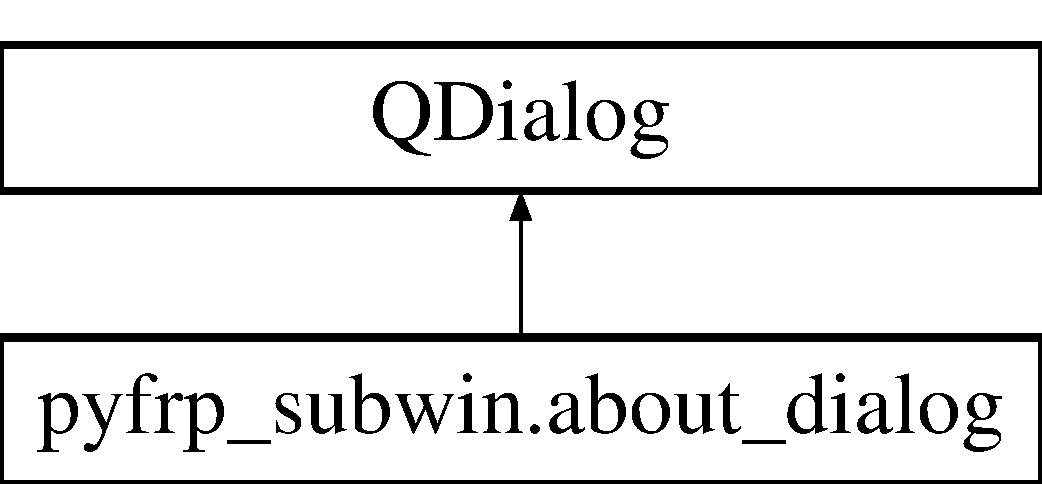
\includegraphics[height=2.000000cm]{classpyfrp__subwin_1_1about__dialog}
\end{center}
\end{figure}
\subsection*{Public Member Functions}
\begin{DoxyCompactItemize}
\item 
\hypertarget{classpyfrp__subwin_1_1about__dialog_ab4c8dc0b27210e6436528b25c3a0d8be}{def {\bfseries \+\_\+\+\_\+init\+\_\+\+\_\+}}\label{classpyfrp__subwin_1_1about__dialog_ab4c8dc0b27210e6436528b25c3a0d8be}

\item 
\hypertarget{classpyfrp__subwin_1_1about__dialog_ac1724af81a159443365b932aff8d052a}{def {\bfseries Open\+U\+R\+L}}\label{classpyfrp__subwin_1_1about__dialog_ac1724af81a159443365b932aff8d052a}

\item 
\hypertarget{classpyfrp__subwin_1_1about__dialog_a6e78b9d56a43afeeb1249e709c24ba0e}{def {\bfseries cancel}}\label{classpyfrp__subwin_1_1about__dialog_a6e78b9d56a43afeeb1249e709c24ba0e}

\end{DoxyCompactItemize}
\subsection*{Public Attributes}
\begin{DoxyCompactItemize}
\item 
\hypertarget{classpyfrp__subwin_1_1about__dialog_a177c3f25afed3cf54a55c44859e026d8}{{\bfseries lbl\+\_\+name}}\label{classpyfrp__subwin_1_1about__dialog_a177c3f25afed3cf54a55c44859e026d8}

\item 
\hypertarget{classpyfrp__subwin_1_1about__dialog_a03731321535589d871c232d24d71e439}{{\bfseries lbl\+\_\+author}}\label{classpyfrp__subwin_1_1about__dialog_a03731321535589d871c232d24d71e439}

\item 
\hypertarget{classpyfrp__subwin_1_1about__dialog_ab773f260bf593aeb2993ed1ea425ba8a}{{\bfseries lbl\+\_\+website}}\label{classpyfrp__subwin_1_1about__dialog_ab773f260bf593aeb2993ed1ea425ba8a}

\item 
\hypertarget{classpyfrp__subwin_1_1about__dialog_a77fce1160b4d997525d3e03201e27c77}{{\bfseries btn\+\_\+cancel}}\label{classpyfrp__subwin_1_1about__dialog_a77fce1160b4d997525d3e03201e27c77}

\item 
\hypertarget{classpyfrp__subwin_1_1about__dialog_a7732047e1d9096b48f17dd23c2a73ce6}{{\bfseries vbox}}\label{classpyfrp__subwin_1_1about__dialog_a7732047e1d9096b48f17dd23c2a73ce6}

\end{DoxyCompactItemize}


The documentation for this class was generated from the following file\+:\begin{DoxyCompactItemize}
\item 
/home/alex\+\_\+loc/\+Documents/\+Research/\+Py\+F\+R\+A\+P/\+Code/pyfrp\+\_\+subwin.\+py\end{DoxyCompactItemize}

\hypertarget{classpyfrp__subwin_1_1analysis__dialog}{\section{pyfrp\+\_\+subwin.\+analysis\+\_\+dialog Class Reference}
\label{classpyfrp__subwin_1_1analysis__dialog}\index{pyfrp\+\_\+subwin.\+analysis\+\_\+dialog@{pyfrp\+\_\+subwin.\+analysis\+\_\+dialog}}
}
Inheritance diagram for pyfrp\+\_\+subwin.\+analysis\+\_\+dialog\+:\begin{figure}[H]
\begin{center}
\leavevmode
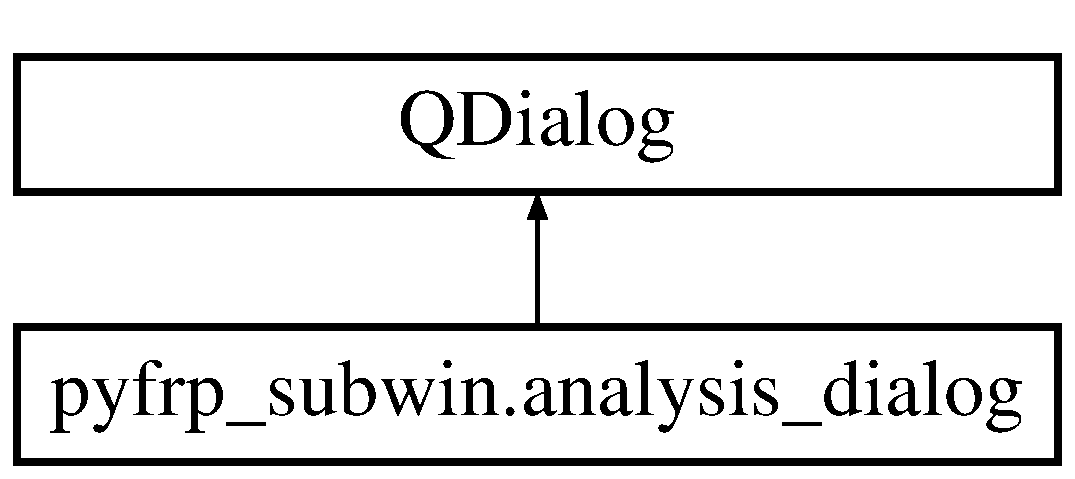
\includegraphics[height=2.000000cm]{classpyfrp__subwin_1_1analysis__dialog}
\end{center}
\end{figure}
\subsection*{Public Member Functions}
\begin{DoxyCompactItemize}
\item 
\hypertarget{classpyfrp__subwin_1_1analysis__dialog_aa3d0436cc0d7e95f1636aea80ec5f86f}{def {\bfseries \+\_\+\+\_\+init\+\_\+\+\_\+}}\label{classpyfrp__subwin_1_1analysis__dialog_aa3d0436cc0d7e95f1636aea80ec5f86f}

\item 
\hypertarget{classpyfrp__subwin_1_1analysis__dialog_a67f4caa5a7de12e4aa65d21e9b2b7259}{def {\bfseries check\+\_\+norm\+\_\+by\+\_\+pre}}\label{classpyfrp__subwin_1_1analysis__dialog_a67f4caa5a7de12e4aa65d21e9b2b7259}

\item 
\hypertarget{classpyfrp__subwin_1_1analysis__dialog_ab6821318dbbc773688becd7e5aa3ea68}{def {\bfseries check\+\_\+img\+\_\+in\+\_\+domain}}\label{classpyfrp__subwin_1_1analysis__dialog_ab6821318dbbc773688becd7e5aa3ea68}

\item 
\hypertarget{classpyfrp__subwin_1_1analysis__dialog_ab377191d3be502dbec6fc20d81cd1780}{def {\bfseries check\+\_\+add\+\_\+rim}}\label{classpyfrp__subwin_1_1analysis__dialog_ab377191d3be502dbec6fc20d81cd1780}

\item 
\hypertarget{classpyfrp__subwin_1_1analysis__dialog_a279a1cd762c69bef256b1adaea856ad2}{def {\bfseries check\+\_\+add\+\_\+rim\+\_\+from\+\_\+radius}}\label{classpyfrp__subwin_1_1analysis__dialog_a279a1cd762c69bef256b1adaea856ad2}

\item 
\hypertarget{classpyfrp__subwin_1_1analysis__dialog_a226810999aaa1043948ca95cd080f401}{def {\bfseries check\+\_\+conc\+\_\+rim}}\label{classpyfrp__subwin_1_1analysis__dialog_a226810999aaa1043948ca95cd080f401}

\item 
\hypertarget{classpyfrp__subwin_1_1analysis__dialog_a78711f1534ef1b91f95945424cb6c3ba}{def {\bfseries check\+\_\+debug}}\label{classpyfrp__subwin_1_1analysis__dialog_a78711f1534ef1b91f95945424cb6c3ba}

\item 
\hypertarget{classpyfrp__subwin_1_1analysis__dialog_a3b5a2ef16ebc05b4a85162aaa140ec19}{def {\bfseries set\+\_\+conc\+\_\+rim}}\label{classpyfrp__subwin_1_1analysis__dialog_a3b5a2ef16ebc05b4a85162aaa140ec19}

\item 
\hypertarget{classpyfrp__subwin_1_1analysis__dialog_a928f536b357e361bf4d7121ebf695804}{def {\bfseries set\+\_\+rim}}\label{classpyfrp__subwin_1_1analysis__dialog_a928f536b357e361bf4d7121ebf695804}

\item 
\hypertarget{classpyfrp__subwin_1_1analysis__dialog_abf66e95f9b1b68e76273c4210ed8900b}{def {\bfseries set\+\_\+preimage}}\label{classpyfrp__subwin_1_1analysis__dialog_abf66e95f9b1b68e76273c4210ed8900b}

\item 
\hypertarget{classpyfrp__subwin_1_1analysis__dialog_ade369aca855e304bd449e03afc59ca8b}{def {\bfseries done\+\_\+pressed}}\label{classpyfrp__subwin_1_1analysis__dialog_ade369aca855e304bd449e03afc59ca8b}

\end{DoxyCompactItemize}
\subsection*{Public Attributes}
\begin{DoxyCompactItemize}
\item 
\hypertarget{classpyfrp__subwin_1_1analysis__dialog_a4ed1d588d16010032f04557c038ab653}{{\bfseries embryo}}\label{classpyfrp__subwin_1_1analysis__dialog_a4ed1d588d16010032f04557c038ab653}

\item 
\hypertarget{classpyfrp__subwin_1_1analysis__dialog_a1ed351304061d4d8a8180e4b6a285868}{{\bfseries btn\+\_\+done}}\label{classpyfrp__subwin_1_1analysis__dialog_a1ed351304061d4d8a8180e4b6a285868}

\item 
\hypertarget{classpyfrp__subwin_1_1analysis__dialog_a319cc3fe0a01062f5fdf69463953f875}{{\bfseries btn\+\_\+preimage}}\label{classpyfrp__subwin_1_1analysis__dialog_a319cc3fe0a01062f5fdf69463953f875}

\item 
\hypertarget{classpyfrp__subwin_1_1analysis__dialog_aa74ea5d2234131f9f0dc4cb45d446111}{{\bfseries lbl\+\_\+pre}}\label{classpyfrp__subwin_1_1analysis__dialog_aa74ea5d2234131f9f0dc4cb45d446111}

\item 
\hypertarget{classpyfrp__subwin_1_1analysis__dialog_a0d429199af58951ed3840eef83a8dc7c}{{\bfseries lbl\+\_\+rim\+\_\+handling}}\label{classpyfrp__subwin_1_1analysis__dialog_a0d429199af58951ed3840eef83a8dc7c}

\item 
\hypertarget{classpyfrp__subwin_1_1analysis__dialog_a4ac09909dcbb752c03e4f29628acd36a}{{\bfseries lbl\+\_\+debugging}}\label{classpyfrp__subwin_1_1analysis__dialog_a4ac09909dcbb752c03e4f29628acd36a}

\item 
\hypertarget{classpyfrp__subwin_1_1analysis__dialog_a3143ad7cbe86235f990ffca3478cdf2f}{{\bfseries lbl\+\_\+rim}}\label{classpyfrp__subwin_1_1analysis__dialog_a3143ad7cbe86235f990ffca3478cdf2f}

\item 
\hypertarget{classpyfrp__subwin_1_1analysis__dialog_adaf4b5ea2c1832ac927be604c98462a2}{{\bfseries lbl\+\_\+norm\+\_\+by\+\_\+pre}}\label{classpyfrp__subwin_1_1analysis__dialog_adaf4b5ea2c1832ac927be604c98462a2}

\item 
\hypertarget{classpyfrp__subwin_1_1analysis__dialog_a2b32aa70b0e95544b93927b1640b511b}{{\bfseries lbl\+\_\+preimage}}\label{classpyfrp__subwin_1_1analysis__dialog_a2b32aa70b0e95544b93927b1640b511b}

\item 
\hypertarget{classpyfrp__subwin_1_1analysis__dialog_ad9af410441e853c72efdee83b5d58ee6}{{\bfseries lbl\+\_\+img\+\_\+in\+\_\+domain}}\label{classpyfrp__subwin_1_1analysis__dialog_ad9af410441e853c72efdee83b5d58ee6}

\item 
\hypertarget{classpyfrp__subwin_1_1analysis__dialog_ac16ffafbfe5febbcb7f85829923084c9}{{\bfseries lbl\+\_\+add\+\_\+rim\+\_\+from\+\_\+radius}}\label{classpyfrp__subwin_1_1analysis__dialog_ac16ffafbfe5febbcb7f85829923084c9}

\item 
\hypertarget{classpyfrp__subwin_1_1analysis__dialog_a22f9ae4d192f45f4d2e3c1aedd93cd61}{{\bfseries lbl\+\_\+add\+\_\+rim}}\label{classpyfrp__subwin_1_1analysis__dialog_a22f9ae4d192f45f4d2e3c1aedd93cd61}

\item 
\hypertarget{classpyfrp__subwin_1_1analysis__dialog_a9ddc426f43717cc319ddd8473667bbab}{{\bfseries lbl\+\_\+debug}}\label{classpyfrp__subwin_1_1analysis__dialog_a9ddc426f43717cc319ddd8473667bbab}

\item 
\hypertarget{classpyfrp__subwin_1_1analysis__dialog_aeaac5d78a87dc163970de01317b5975d}{{\bfseries lbl\+\_\+use\+\_\+conc\+\_\+rim}}\label{classpyfrp__subwin_1_1analysis__dialog_aeaac5d78a87dc163970de01317b5975d}

\item 
\hypertarget{classpyfrp__subwin_1_1analysis__dialog_aecfc25495c6cc329dce9eea2472a9bf2}{{\bfseries lbl\+\_\+conc\+\_\+rim}}\label{classpyfrp__subwin_1_1analysis__dialog_aecfc25495c6cc329dce9eea2472a9bf2}

\item 
\hypertarget{classpyfrp__subwin_1_1analysis__dialog_ac7d89a461fd44e162879a1f4427cc1f8}{{\bfseries cb\+\_\+debug}}\label{classpyfrp__subwin_1_1analysis__dialog_ac7d89a461fd44e162879a1f4427cc1f8}

\item 
\hypertarget{classpyfrp__subwin_1_1analysis__dialog_a86266fd8f68ee768cd527b1239cd88d9}{{\bfseries cb\+\_\+img\+\_\+in\+\_\+domain}}\label{classpyfrp__subwin_1_1analysis__dialog_a86266fd8f68ee768cd527b1239cd88d9}

\item 
\hypertarget{classpyfrp__subwin_1_1analysis__dialog_a65904538459cbc45d8cb01167a6fbfec}{{\bfseries cb\+\_\+add\+\_\+rim}}\label{classpyfrp__subwin_1_1analysis__dialog_a65904538459cbc45d8cb01167a6fbfec}

\item 
\hypertarget{classpyfrp__subwin_1_1analysis__dialog_a145b7892ff365c8cfb35a1808188a58a}{{\bfseries cb\+\_\+add\+\_\+rim\+\_\+from\+\_\+radius}}\label{classpyfrp__subwin_1_1analysis__dialog_a145b7892ff365c8cfb35a1808188a58a}

\item 
\hypertarget{classpyfrp__subwin_1_1analysis__dialog_a3735740ad0876aff6b12becf5116b9a5}{{\bfseries cb\+\_\+conc\+\_\+rim}}\label{classpyfrp__subwin_1_1analysis__dialog_a3735740ad0876aff6b12becf5116b9a5}

\item 
\hypertarget{classpyfrp__subwin_1_1analysis__dialog_a66ff91635b5c04e31521b752646df6a6}{{\bfseries cb\+\_\+norm\+\_\+by\+\_\+pre}}\label{classpyfrp__subwin_1_1analysis__dialog_a66ff91635b5c04e31521b752646df6a6}

\item 
\hypertarget{classpyfrp__subwin_1_1analysis__dialog_a56404cbad095635ee47ede547eb51f58}{{\bfseries qle\+\_\+conc\+\_\+rim}}\label{classpyfrp__subwin_1_1analysis__dialog_a56404cbad095635ee47ede547eb51f58}

\item 
\hypertarget{classpyfrp__subwin_1_1analysis__dialog_a43e561c53dc8fbda7ef8b2f9d4d3f051}{{\bfseries qle\+\_\+rim}}\label{classpyfrp__subwin_1_1analysis__dialog_a43e561c53dc8fbda7ef8b2f9d4d3f051}

\item 
\hypertarget{classpyfrp__subwin_1_1analysis__dialog_a72fb308fa0f53a11f6067cddfafe41fa}{{\bfseries double\+\_\+valid}}\label{classpyfrp__subwin_1_1analysis__dialog_a72fb308fa0f53a11f6067cddfafe41fa}

\end{DoxyCompactItemize}


The documentation for this class was generated from the following file\+:\begin{DoxyCompactItemize}
\item 
/home/alex\+\_\+loc/\+Documents/\+Research/\+Py\+F\+R\+A\+P/\+Code/pyfrp\+\_\+subwin.\+py\end{DoxyCompactItemize}

\hypertarget{classpyfrp__subwin_1_1analyze__all__prog}{\section{pyfrp\+\_\+subwin.\+analyze\+\_\+all\+\_\+prog Class Reference}
\label{classpyfrp__subwin_1_1analyze__all__prog}\index{pyfrp\+\_\+subwin.\+analyze\+\_\+all\+\_\+prog@{pyfrp\+\_\+subwin.\+analyze\+\_\+all\+\_\+prog}}
}
Inheritance diagram for pyfrp\+\_\+subwin.\+analyze\+\_\+all\+\_\+prog\+:\begin{figure}[H]
\begin{center}
\leavevmode
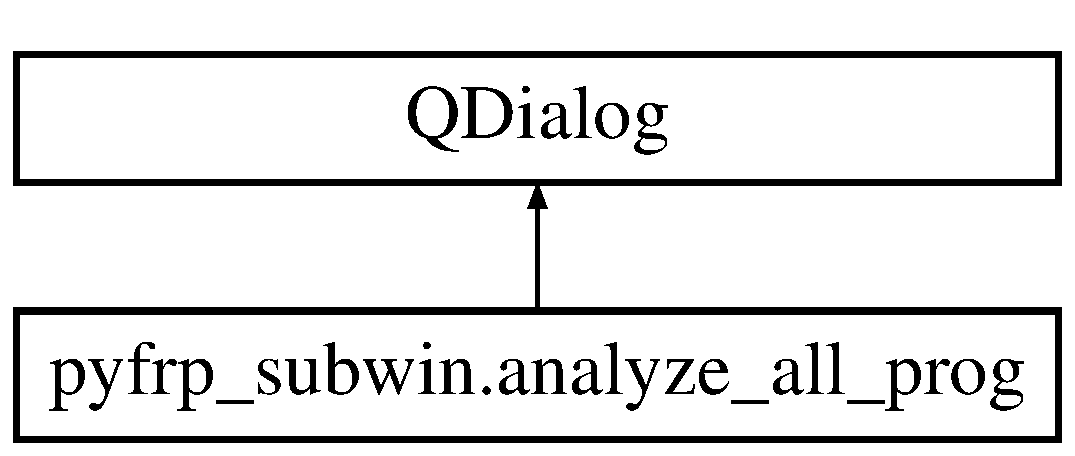
\includegraphics[height=2.000000cm]{classpyfrp__subwin_1_1analyze__all__prog}
\end{center}
\end{figure}
\subsection*{Public Member Functions}
\begin{DoxyCompactItemize}
\item 
\hypertarget{classpyfrp__subwin_1_1analyze__all__prog_a2e23b0e0d707d0d412ed59caa561a145}{def {\bfseries \+\_\+\+\_\+init\+\_\+\+\_\+}}\label{classpyfrp__subwin_1_1analyze__all__prog_a2e23b0e0d707d0d412ed59caa561a145}

\item 
\hypertarget{classpyfrp__subwin_1_1analyze__all__prog_ad7a7103733ac63306032980b27760c13}{def {\bfseries cancel\+\_\+analysis}}\label{classpyfrp__subwin_1_1analyze__all__prog_ad7a7103733ac63306032980b27760c13}

\end{DoxyCompactItemize}
\subsection*{Public Attributes}
\begin{DoxyCompactItemize}
\item 
\hypertarget{classpyfrp__subwin_1_1analyze__all__prog_a4c80819f1c4529c4db6ce364898b994a}{{\bfseries molecule}}\label{classpyfrp__subwin_1_1analyze__all__prog_a4c80819f1c4529c4db6ce364898b994a}

\item 
\hypertarget{classpyfrp__subwin_1_1analyze__all__prog_ae3f9193bfd66680782123fcccdb8c0b9}{{\bfseries lbl\+\_\+name}}\label{classpyfrp__subwin_1_1analyze__all__prog_ae3f9193bfd66680782123fcccdb8c0b9}

\item 
\hypertarget{classpyfrp__subwin_1_1analyze__all__prog_a334f4d57ba7d2522b125af9a7ef5765e}{{\bfseries btn\+\_\+cancel}}\label{classpyfrp__subwin_1_1analyze__all__prog_a334f4d57ba7d2522b125af9a7ef5765e}

\item 
\hypertarget{classpyfrp__subwin_1_1analyze__all__prog_ad441a8233cea8bb781306773d1277432}{{\bfseries progressbar}}\label{classpyfrp__subwin_1_1analyze__all__prog_ad441a8233cea8bb781306773d1277432}

\item 
\hypertarget{classpyfrp__subwin_1_1analyze__all__prog_a8b666a1cb3a06958b4b18a2fb3673727}{{\bfseries vbox}}\label{classpyfrp__subwin_1_1analyze__all__prog_a8b666a1cb3a06958b4b18a2fb3673727}

\end{DoxyCompactItemize}


The documentation for this class was generated from the following file\+:\begin{DoxyCompactItemize}
\item 
/home/alex\+\_\+loc/\+Documents/\+Research/\+Py\+F\+R\+A\+P/\+Code/pyfrp\+\_\+subwin.\+py\end{DoxyCompactItemize}

\hypertarget{classpyfrp__subwin_1_1analyze__all__thread}{\section{pyfrp\+\_\+subwin.\+analyze\+\_\+all\+\_\+thread Class Reference}
\label{classpyfrp__subwin_1_1analyze__all__thread}\index{pyfrp\+\_\+subwin.\+analyze\+\_\+all\+\_\+thread@{pyfrp\+\_\+subwin.\+analyze\+\_\+all\+\_\+thread}}
}
Inheritance diagram for pyfrp\+\_\+subwin.\+analyze\+\_\+all\+\_\+thread\+:\begin{figure}[H]
\begin{center}
\leavevmode
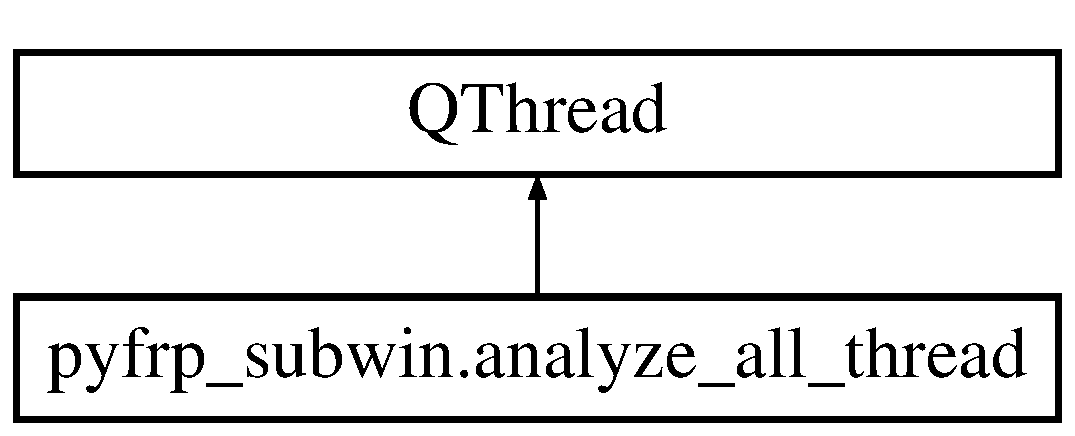
\includegraphics[height=2.000000cm]{classpyfrp__subwin_1_1analyze__all__thread}
\end{center}
\end{figure}
\subsection*{Public Member Functions}
\begin{DoxyCompactItemize}
\item 
\hypertarget{classpyfrp__subwin_1_1analyze__all__thread_aec9f4edfc0e781f2e3b20c24be00a852}{def {\bfseries \+\_\+\+\_\+init\+\_\+\+\_\+}}\label{classpyfrp__subwin_1_1analyze__all__thread_aec9f4edfc0e781f2e3b20c24be00a852}

\item 
\hypertarget{classpyfrp__subwin_1_1analyze__all__thread_adeaab23c3751b0d5f1388be250571ccb}{def {\bfseries \+\_\+\+\_\+del\+\_\+\+\_\+}}\label{classpyfrp__subwin_1_1analyze__all__thread_adeaab23c3751b0d5f1388be250571ccb}

\item 
\hypertarget{classpyfrp__subwin_1_1analyze__all__thread_a8973a06e1d896f91a46a8f82e0711bd3}{def {\bfseries run}}\label{classpyfrp__subwin_1_1analyze__all__thread_a8973a06e1d896f91a46a8f82e0711bd3}

\end{DoxyCompactItemize}
\subsection*{Public Attributes}
\begin{DoxyCompactItemize}
\item 
\hypertarget{classpyfrp__subwin_1_1analyze__all__thread_a68f691af707b243976351f638f329ea0}{{\bfseries molecule}}\label{classpyfrp__subwin_1_1analyze__all__thread_a68f691af707b243976351f638f329ea0}

\end{DoxyCompactItemize}
\subsection*{Static Public Attributes}
\begin{DoxyCompactItemize}
\item 
\hypertarget{classpyfrp__subwin_1_1analyze__all__thread_a7e107c5d6871f05837e5f03c38cbdc69}{tuple {\bfseries task\+Finished} = Qt\+Core.\+pyqt\+Signal()}\label{classpyfrp__subwin_1_1analyze__all__thread_a7e107c5d6871f05837e5f03c38cbdc69}

\item 
\hypertarget{classpyfrp__subwin_1_1analyze__all__thread_a2fa1a91163d761b3c71dafec4e846851}{tuple {\bfseries prog\+\_\+signal} = Qt\+Core.\+pyqt\+Signal(int,int)}\label{classpyfrp__subwin_1_1analyze__all__thread_a2fa1a91163d761b3c71dafec4e846851}

\end{DoxyCompactItemize}


The documentation for this class was generated from the following file\+:\begin{DoxyCompactItemize}
\item 
/home/alex\+\_\+loc/\+Documents/\+Research/\+Py\+F\+R\+A\+P/\+Code/pyfrp\+\_\+subwin.\+py\end{DoxyCompactItemize}

\hypertarget{classpyfrp__subwin_1_1analyze__prog}{\section{pyfrp\+\_\+subwin.\+analyze\+\_\+prog Class Reference}
\label{classpyfrp__subwin_1_1analyze__prog}\index{pyfrp\+\_\+subwin.\+analyze\+\_\+prog@{pyfrp\+\_\+subwin.\+analyze\+\_\+prog}}
}
Inheritance diagram for pyfrp\+\_\+subwin.\+analyze\+\_\+prog\+:\begin{figure}[H]
\begin{center}
\leavevmode
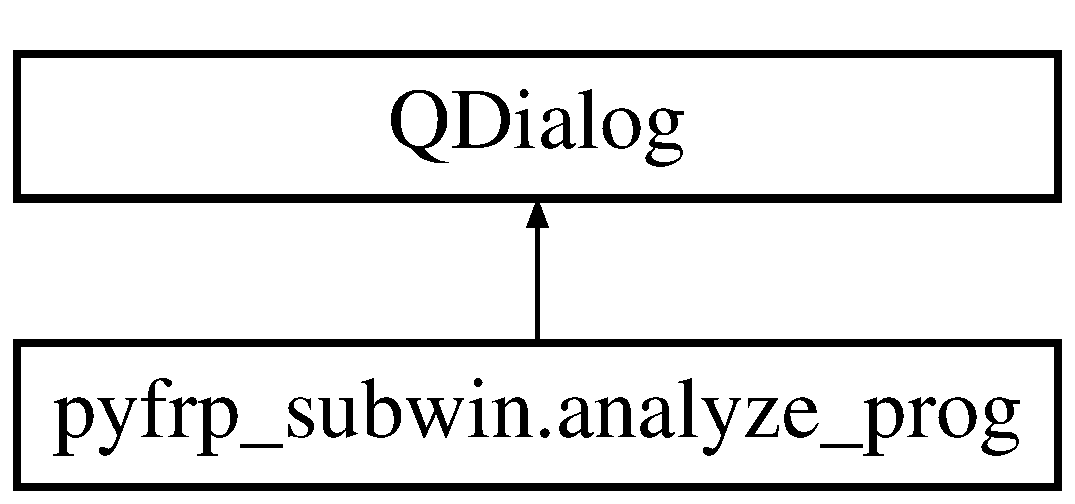
\includegraphics[height=2.000000cm]{classpyfrp__subwin_1_1analyze__prog}
\end{center}
\end{figure}
\subsection*{Public Member Functions}
\begin{DoxyCompactItemize}
\item 
\hypertarget{classpyfrp__subwin_1_1analyze__prog_a8fee5e11087e59f9070f967292228dfc}{def {\bfseries \+\_\+\+\_\+init\+\_\+\+\_\+}}\label{classpyfrp__subwin_1_1analyze__prog_a8fee5e11087e59f9070f967292228dfc}

\item 
\hypertarget{classpyfrp__subwin_1_1analyze__prog_a453ee0a13df2e43015898ece63498d85}{def {\bfseries cancel\+\_\+analysis}}\label{classpyfrp__subwin_1_1analyze__prog_a453ee0a13df2e43015898ece63498d85}

\end{DoxyCompactItemize}
\subsection*{Public Attributes}
\begin{DoxyCompactItemize}
\item 
\hypertarget{classpyfrp__subwin_1_1analyze__prog_a4b459df088c186083d54431e81ddd3c4}{{\bfseries lbl\+\_\+name}}\label{classpyfrp__subwin_1_1analyze__prog_a4b459df088c186083d54431e81ddd3c4}

\item 
\hypertarget{classpyfrp__subwin_1_1analyze__prog_a5ef873e7e15e686fa18a2fd0c1f73909}{{\bfseries btn\+\_\+cancel}}\label{classpyfrp__subwin_1_1analyze__prog_a5ef873e7e15e686fa18a2fd0c1f73909}

\item 
\hypertarget{classpyfrp__subwin_1_1analyze__prog_ac76f125873f7749076674dc7a3416734}{{\bfseries progressbar}}\label{classpyfrp__subwin_1_1analyze__prog_ac76f125873f7749076674dc7a3416734}

\item 
\hypertarget{classpyfrp__subwin_1_1analyze__prog_a843d47d141e4a9ffc811fa3997a6dbed}{{\bfseries vbox}}\label{classpyfrp__subwin_1_1analyze__prog_a843d47d141e4a9ffc811fa3997a6dbed}

\end{DoxyCompactItemize}


The documentation for this class was generated from the following file\+:\begin{DoxyCompactItemize}
\item 
/home/alex\+\_\+loc/\+Documents/\+Research/\+Py\+F\+R\+A\+P/\+Code/pyfrp\+\_\+subwin.\+py\end{DoxyCompactItemize}

\hypertarget{classpyfrp__subwin_1_1analyze__thread}{\section{pyfrp\+\_\+subwin.\+analyze\+\_\+thread Class Reference}
\label{classpyfrp__subwin_1_1analyze__thread}\index{pyfrp\+\_\+subwin.\+analyze\+\_\+thread@{pyfrp\+\_\+subwin.\+analyze\+\_\+thread}}
}
Inheritance diagram for pyfrp\+\_\+subwin.\+analyze\+\_\+thread\+:\begin{figure}[H]
\begin{center}
\leavevmode
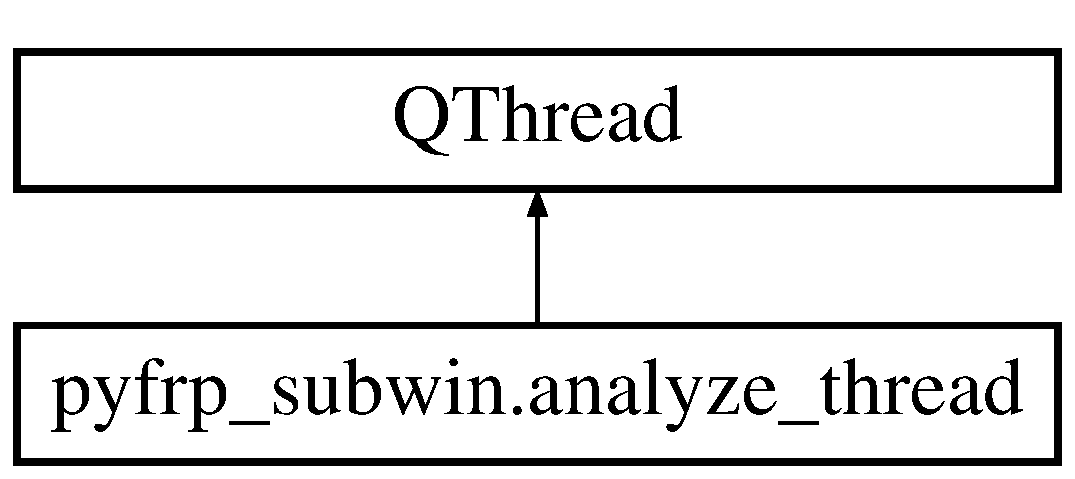
\includegraphics[height=2.000000cm]{classpyfrp__subwin_1_1analyze__thread}
\end{center}
\end{figure}
\subsection*{Public Member Functions}
\begin{DoxyCompactItemize}
\item 
\hypertarget{classpyfrp__subwin_1_1analyze__thread_a7024f889bbc687ca1dccb843d4580f25}{def {\bfseries \+\_\+\+\_\+init\+\_\+\+\_\+}}\label{classpyfrp__subwin_1_1analyze__thread_a7024f889bbc687ca1dccb843d4580f25}

\item 
\hypertarget{classpyfrp__subwin_1_1analyze__thread_aca9448e77c769805eacba8fdae872bd2}{def {\bfseries \+\_\+\+\_\+del\+\_\+\+\_\+}}\label{classpyfrp__subwin_1_1analyze__thread_aca9448e77c769805eacba8fdae872bd2}

\item 
\hypertarget{classpyfrp__subwin_1_1analyze__thread_aeda52ff84426e5f8ac275425749d381b}{def {\bfseries run}}\label{classpyfrp__subwin_1_1analyze__thread_aeda52ff84426e5f8ac275425749d381b}

\end{DoxyCompactItemize}
\subsection*{Public Attributes}
\begin{DoxyCompactItemize}
\item 
\hypertarget{classpyfrp__subwin_1_1analyze__thread_a2d3d122beee61b4ab632a3ea50d2b39e}{{\bfseries embryo}}\label{classpyfrp__subwin_1_1analyze__thread_a2d3d122beee61b4ab632a3ea50d2b39e}

\end{DoxyCompactItemize}
\subsection*{Static Public Attributes}
\begin{DoxyCompactItemize}
\item 
\hypertarget{classpyfrp__subwin_1_1analyze__thread_a10302ef773f3c87e6b21daeeaceb50cb}{tuple {\bfseries task\+Finished} = Qt\+Core.\+pyqt\+Signal()}\label{classpyfrp__subwin_1_1analyze__thread_a10302ef773f3c87e6b21daeeaceb50cb}

\item 
\hypertarget{classpyfrp__subwin_1_1analyze__thread_adbc6e93966305a425126903c1e29ba2f}{tuple {\bfseries prog\+\_\+signal} = Qt\+Core.\+pyqt\+Signal(int)}\label{classpyfrp__subwin_1_1analyze__thread_adbc6e93966305a425126903c1e29ba2f}

\end{DoxyCompactItemize}


The documentation for this class was generated from the following file\+:\begin{DoxyCompactItemize}
\item 
/home/alex\+\_\+loc/\+Documents/\+Research/\+Py\+F\+R\+A\+P/\+Code/pyfrp\+\_\+subwin.\+py\end{DoxyCompactItemize}

\hypertarget{classpyfrp__subwin_1_1dataset__dialog}{\section{pyfrp\+\_\+subwin.\+dataset\+\_\+dialog Class Reference}
\label{classpyfrp__subwin_1_1dataset__dialog}\index{pyfrp\+\_\+subwin.\+dataset\+\_\+dialog@{pyfrp\+\_\+subwin.\+dataset\+\_\+dialog}}
}
Inheritance diagram for pyfrp\+\_\+subwin.\+dataset\+\_\+dialog\+:\begin{figure}[H]
\begin{center}
\leavevmode
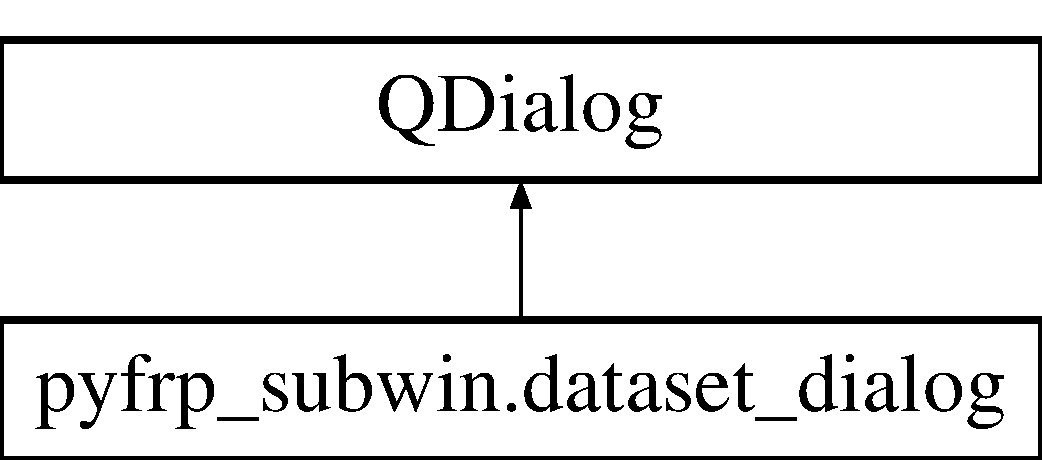
\includegraphics[height=2.000000cm]{classpyfrp__subwin_1_1dataset__dialog}
\end{center}
\end{figure}
\subsection*{Public Member Functions}
\begin{DoxyCompactItemize}
\item 
\hypertarget{classpyfrp__subwin_1_1dataset__dialog_a139fd0b64dba550c6848609409eeb81c}{def {\bfseries \+\_\+\+\_\+init\+\_\+\+\_\+}}\label{classpyfrp__subwin_1_1dataset__dialog_a139fd0b64dba550c6848609409eeb81c}

\item 
\hypertarget{classpyfrp__subwin_1_1dataset__dialog_ae2f6121597dd804ce4dbebee6e036e56}{def {\bfseries create\+\_\+frame}}\label{classpyfrp__subwin_1_1dataset__dialog_ae2f6121597dd804ce4dbebee6e036e56}

\item 
\hypertarget{classpyfrp__subwin_1_1dataset__dialog_adbf5e6668280041d014f18c0f10741bd}{def {\bfseries sel\+\_\+datafolder}}\label{classpyfrp__subwin_1_1dataset__dialog_adbf5e6668280041d014f18c0f10741bd}

\item 
\hypertarget{classpyfrp__subwin_1_1dataset__dialog_a2f9e730b4cb94c09577f2f83375f29ab}{def {\bfseries sel\+\_\+ft}}\label{classpyfrp__subwin_1_1dataset__dialog_a2f9e730b4cb94c09577f2f83375f29ab}

\item 
\hypertarget{classpyfrp__subwin_1_1dataset__dialog_a2e57aebd3af92b2b6a1bafd6e931cad8}{def {\bfseries sel\+\_\+enc}}\label{classpyfrp__subwin_1_1dataset__dialog_a2e57aebd3af92b2b6a1bafd6e931cad8}

\item 
\hypertarget{classpyfrp__subwin_1_1dataset__dialog_a64e2004b8cc285ccc9f738039e312151}{def {\bfseries set\+\_\+name}}\label{classpyfrp__subwin_1_1dataset__dialog_a64e2004b8cc285ccc9f738039e312151}

\item 
\hypertarget{classpyfrp__subwin_1_1dataset__dialog_acd3a21529cbffa3782cbb3116c33f839}{def {\bfseries set\+\_\+framerate}}\label{classpyfrp__subwin_1_1dataset__dialog_acd3a21529cbffa3782cbb3116c33f839}

\item 
\hypertarget{classpyfrp__subwin_1_1dataset__dialog_ad720c88fbfd0d5048c51416500cd194b}{def {\bfseries set\+\_\+tstart}}\label{classpyfrp__subwin_1_1dataset__dialog_ad720c88fbfd0d5048c51416500cd194b}

\item 
\hypertarget{classpyfrp__subwin_1_1dataset__dialog_ae4634333e8aa22c9ba886f600b2e32d5}{def {\bfseries set\+\_\+res}}\label{classpyfrp__subwin_1_1dataset__dialog_ae4634333e8aa22c9ba886f600b2e32d5}

\item 
\hypertarget{classpyfrp__subwin_1_1dataset__dialog_a3f9a6ca0934fbc3915b9f2cb886af392}{def {\bfseries set\+\_\+radius}}\label{classpyfrp__subwin_1_1dataset__dialog_a3f9a6ca0934fbc3915b9f2cb886af392}

\item 
\hypertarget{classpyfrp__subwin_1_1dataset__dialog_ad5b06fe05d1d93fcb6fde64c6ab0a8d9}{def {\bfseries set\+\_\+center\+\_\+x}}\label{classpyfrp__subwin_1_1dataset__dialog_ad5b06fe05d1d93fcb6fde64c6ab0a8d9}

\item 
\hypertarget{classpyfrp__subwin_1_1dataset__dialog_ab070512770d2f14f28a82c214234ad7c}{def {\bfseries set\+\_\+center\+\_\+y}}\label{classpyfrp__subwin_1_1dataset__dialog_ab070512770d2f14f28a82c214234ad7c}

\item 
\hypertarget{classpyfrp__subwin_1_1dataset__dialog_afb9400487263ef59736ff0e7ab5e0428}{def {\bfseries set\+\_\+sidelength}}\label{classpyfrp__subwin_1_1dataset__dialog_afb9400487263ef59736ff0e7ab5e0428}

\item 
\hypertarget{classpyfrp__subwin_1_1dataset__dialog_a8f2c72cbd4ec720a6720057fcb15649b}{def {\bfseries set\+\_\+offset\+\_\+x}}\label{classpyfrp__subwin_1_1dataset__dialog_a8f2c72cbd4ec720a6720057fcb15649b}

\item 
\hypertarget{classpyfrp__subwin_1_1dataset__dialog_a8a52071f9a7dd869dbda4b19a8ae25af}{def {\bfseries set\+\_\+offset\+\_\+y}}\label{classpyfrp__subwin_1_1dataset__dialog_a8a52071f9a7dd869dbda4b19a8ae25af}

\item 
\hypertarget{classpyfrp__subwin_1_1dataset__dialog_abbcad6120f5f2d85c5fc2ba8e33c7af0}{def {\bfseries update\+\_\+tvec}}\label{classpyfrp__subwin_1_1dataset__dialog_abbcad6120f5f2d85c5fc2ba8e33c7af0}

\item 
\hypertarget{classpyfrp__subwin_1_1dataset__dialog_a1afa8a56c98021b6fb64ec5e7ac62a73}{def {\bfseries update\+\_\+qles}}\label{classpyfrp__subwin_1_1dataset__dialog_a1afa8a56c98021b6fb64ec5e7ac62a73}

\item 
\hypertarget{classpyfrp__subwin_1_1dataset__dialog_ac428fdc5568c823d8adf7da9ad371877}{def {\bfseries create\+\_\+canvas}}\label{classpyfrp__subwin_1_1dataset__dialog_ac428fdc5568c823d8adf7da9ad371877}

\item 
\hypertarget{classpyfrp__subwin_1_1dataset__dialog_a2100ec437aac30c64bb008e65dcbc3f9}{def {\bfseries draw\+\_\+patches}}\label{classpyfrp__subwin_1_1dataset__dialog_a2100ec437aac30c64bb008e65dcbc3f9}

\item 
\hypertarget{classpyfrp__subwin_1_1dataset__dialog_a00fdd541feb15a7485b6b930b7fdcbf1}{def {\bfseries show\+\_\+img}}\label{classpyfrp__subwin_1_1dataset__dialog_a00fdd541feb15a7485b6b930b7fdcbf1}

\item 
\hypertarget{classpyfrp__subwin_1_1dataset__dialog_a897df1c015cf1bf990098b55849bad14}{def {\bfseries get\+\_\+mouse\+\_\+embr\+\_\+radius}}\label{classpyfrp__subwin_1_1dataset__dialog_a897df1c015cf1bf990098b55849bad14}

\item 
\hypertarget{classpyfrp__subwin_1_1dataset__dialog_a79e09797908f5fb27bac08cab7bff129}{def {\bfseries clear\+\_\+patch\+\_\+canvas}}\label{classpyfrp__subwin_1_1dataset__dialog_a79e09797908f5fb27bac08cab7bff129}

\item 
\hypertarget{classpyfrp__subwin_1_1dataset__dialog_ab6719cd5d778e49ef0007f687e4f4c00}{def {\bfseries clear\+\_\+patch\+\_\+canvas\+\_\+squ}}\label{classpyfrp__subwin_1_1dataset__dialog_ab6719cd5d778e49ef0007f687e4f4c00}

\item 
\hypertarget{classpyfrp__subwin_1_1dataset__dialog_a2c7cf0ae8284b76606e3c8f017f8a8aa}{def {\bfseries done\+\_\+pressed}}\label{classpyfrp__subwin_1_1dataset__dialog_a2c7cf0ae8284b76606e3c8f017f8a8aa}

\end{DoxyCompactItemize}
\subsection*{Public Attributes}
\begin{DoxyCompactItemize}
\item 
\hypertarget{classpyfrp__subwin_1_1dataset__dialog_a19018385e74981ae912ae1acf362c6db}{{\bfseries embryo}}\label{classpyfrp__subwin_1_1dataset__dialog_a19018385e74981ae912ae1acf362c6db}

\item 
\hypertarget{classpyfrp__subwin_1_1dataset__dialog_aee1b62f6afd21f8327530cc6c83a74bf}{{\bfseries dpi}}\label{classpyfrp__subwin_1_1dataset__dialog_aee1b62f6afd21f8327530cc6c83a74bf}

\item 
\hypertarget{classpyfrp__subwin_1_1dataset__dialog_ad11b10c2b971e405a7c797bbd48f222a}{{\bfseries xcoords2}}\label{classpyfrp__subwin_1_1dataset__dialog_ad11b10c2b971e405a7c797bbd48f222a}

\item 
\hypertarget{classpyfrp__subwin_1_1dataset__dialog_a86a4ed31457febfda596ff733c1a9036}{{\bfseries ycoords2}}\label{classpyfrp__subwin_1_1dataset__dialog_a86a4ed31457febfda596ff733c1a9036}

\item 
\hypertarget{classpyfrp__subwin_1_1dataset__dialog_a037afb3e0cb62010abeee0d1b61aa809}{{\bfseries xcoords}}\label{classpyfrp__subwin_1_1dataset__dialog_a037afb3e0cb62010abeee0d1b61aa809}

\item 
\hypertarget{classpyfrp__subwin_1_1dataset__dialog_a460737464c9cf96e8626b4e1f48aaa4b}{{\bfseries ycoords}}\label{classpyfrp__subwin_1_1dataset__dialog_a460737464c9cf96e8626b4e1f48aaa4b}

\item 
\hypertarget{classpyfrp__subwin_1_1dataset__dialog_ad3bd2bfe4bc30584effceeb44eda8a8b}{{\bfseries pts\+\_\+in\+\_\+ax}}\label{classpyfrp__subwin_1_1dataset__dialog_ad3bd2bfe4bc30584effceeb44eda8a8b}

\item 
\hypertarget{classpyfrp__subwin_1_1dataset__dialog_a2e7644e66b7b83e5095332c64bc942f6}{{\bfseries pts\+\_\+in\+\_\+ax2}}\label{classpyfrp__subwin_1_1dataset__dialog_a2e7644e66b7b83e5095332c64bc942f6}

\item 
\hypertarget{classpyfrp__subwin_1_1dataset__dialog_ae36874db3ca588437b2c122d906d1b0f}{{\bfseries btn\+\_\+done}}\label{classpyfrp__subwin_1_1dataset__dialog_ae36874db3ca588437b2c122d906d1b0f}

\item 
\hypertarget{classpyfrp__subwin_1_1dataset__dialog_a05d03461a293407a91fd8eed348900f0}{{\bfseries btn\+\_\+set\+\_\+datafolder}}\label{classpyfrp__subwin_1_1dataset__dialog_a05d03461a293407a91fd8eed348900f0}

\item 
\hypertarget{classpyfrp__subwin_1_1dataset__dialog_a4d26e09a0c1b72e9af6b821352769699}{{\bfseries lbl\+\_\+name}}\label{classpyfrp__subwin_1_1dataset__dialog_a4d26e09a0c1b72e9af6b821352769699}

\item 
\hypertarget{classpyfrp__subwin_1_1dataset__dialog_aea5bf9c6ea0ab33882b347b9474df63b}{{\bfseries lbl\+\_\+name\+\_\+datafolder}}\label{classpyfrp__subwin_1_1dataset__dialog_aea5bf9c6ea0ab33882b347b9474df63b}

\item 
\hypertarget{classpyfrp__subwin_1_1dataset__dialog_a0e98641d51ff0b2bad4da0767cf8550c}{{\bfseries lbl\+\_\+name\+\_\+ft}}\label{classpyfrp__subwin_1_1dataset__dialog_a0e98641d51ff0b2bad4da0767cf8550c}

\item 
\hypertarget{classpyfrp__subwin_1_1dataset__dialog_a0a522ba40cd73281747175caad900786}{{\bfseries lbl\+\_\+name\+\_\+enc}}\label{classpyfrp__subwin_1_1dataset__dialog_a0a522ba40cd73281747175caad900786}

\item 
\hypertarget{classpyfrp__subwin_1_1dataset__dialog_ae6cd2cad557d929d78b7925122116667}{{\bfseries lbl\+\_\+name\+\_\+res}}\label{classpyfrp__subwin_1_1dataset__dialog_ae6cd2cad557d929d78b7925122116667}

\item 
\hypertarget{classpyfrp__subwin_1_1dataset__dialog_a987051e2cbddbcacecdfb7c0d9df1f75}{{\bfseries lbl\+\_\+name\+\_\+radius}}\label{classpyfrp__subwin_1_1dataset__dialog_a987051e2cbddbcacecdfb7c0d9df1f75}

\item 
\hypertarget{classpyfrp__subwin_1_1dataset__dialog_afcdd8b66bcc8636e23ec1f4ebd880199}{{\bfseries lbl\+\_\+name\+\_\+center}}\label{classpyfrp__subwin_1_1dataset__dialog_afcdd8b66bcc8636e23ec1f4ebd880199}

\item 
\hypertarget{classpyfrp__subwin_1_1dataset__dialog_aac0c00f33916f3e7b25df3f56cf55f72}{{\bfseries lbl\+\_\+name\+\_\+offset}}\label{classpyfrp__subwin_1_1dataset__dialog_aac0c00f33916f3e7b25df3f56cf55f72}

\item 
\hypertarget{classpyfrp__subwin_1_1dataset__dialog_a106f92fd84a0df4c1287140ffdb412cd}{{\bfseries lbl\+\_\+name\+\_\+sidelength}}\label{classpyfrp__subwin_1_1dataset__dialog_a106f92fd84a0df4c1287140ffdb412cd}

\item 
\hypertarget{classpyfrp__subwin_1_1dataset__dialog_a1166c135a0fd7e732656de774b9c9889}{{\bfseries lbl\+\_\+name\+\_\+framerate}}\label{classpyfrp__subwin_1_1dataset__dialog_a1166c135a0fd7e732656de774b9c9889}

\item 
\hypertarget{classpyfrp__subwin_1_1dataset__dialog_a9d6c2aa900b97460cb42009303293748}{{\bfseries lbl\+\_\+name\+\_\+nframes}}\label{classpyfrp__subwin_1_1dataset__dialog_a9d6c2aa900b97460cb42009303293748}

\item 
\hypertarget{classpyfrp__subwin_1_1dataset__dialog_a0f6fbc8476f2b060746499c4e702a8cf}{{\bfseries lbl\+\_\+name\+\_\+tstart}}\label{classpyfrp__subwin_1_1dataset__dialog_a0f6fbc8476f2b060746499c4e702a8cf}

\item 
\hypertarget{classpyfrp__subwin_1_1dataset__dialog_a31bfe2d0e94b77c53e5dd296e36adf4a}{{\bfseries lbl\+\_\+name\+\_\+tend}}\label{classpyfrp__subwin_1_1dataset__dialog_a31bfe2d0e94b77c53e5dd296e36adf4a}

\item 
\hypertarget{classpyfrp__subwin_1_1dataset__dialog_a25e1dfdad6ba3540b9daf65baca9eeb0}{{\bfseries lbl\+\_\+datafolder}}\label{classpyfrp__subwin_1_1dataset__dialog_a25e1dfdad6ba3540b9daf65baca9eeb0}

\item 
\hypertarget{classpyfrp__subwin_1_1dataset__dialog_acacc3aa1e052c87fd4cb0b7915bc53e5}{{\bfseries lbl\+\_\+tend}}\label{classpyfrp__subwin_1_1dataset__dialog_acacc3aa1e052c87fd4cb0b7915bc53e5}

\item 
\hypertarget{classpyfrp__subwin_1_1dataset__dialog_af7ed4f5c93265e7d798beb68bf5b71c4}{{\bfseries lbl\+\_\+nframes}}\label{classpyfrp__subwin_1_1dataset__dialog_af7ed4f5c93265e7d798beb68bf5b71c4}

\item 
\hypertarget{classpyfrp__subwin_1_1dataset__dialog_a1de4a665174510cb521524b707b594f9}{{\bfseries combo\+\_\+ft}}\label{classpyfrp__subwin_1_1dataset__dialog_a1de4a665174510cb521524b707b594f9}

\item 
\hypertarget{classpyfrp__subwin_1_1dataset__dialog_aa9900a0e7dd77673c27549c5e2614e3e}{{\bfseries combo\+\_\+enc}}\label{classpyfrp__subwin_1_1dataset__dialog_aa9900a0e7dd77673c27549c5e2614e3e}

\item 
\hypertarget{classpyfrp__subwin_1_1dataset__dialog_a1edc8cadf1dab768d411e710c4e60080}{{\bfseries qle\+\_\+name}}\label{classpyfrp__subwin_1_1dataset__dialog_a1edc8cadf1dab768d411e710c4e60080}

\item 
\hypertarget{classpyfrp__subwin_1_1dataset__dialog_adf8e7269943cf34dfcc6b5dee7ea5758}{{\bfseries qle\+\_\+framerate}}\label{classpyfrp__subwin_1_1dataset__dialog_adf8e7269943cf34dfcc6b5dee7ea5758}

\item 
\hypertarget{classpyfrp__subwin_1_1dataset__dialog_a27f683242429784a9f51c96c9960636d}{{\bfseries qle\+\_\+tstart}}\label{classpyfrp__subwin_1_1dataset__dialog_a27f683242429784a9f51c96c9960636d}

\item 
\hypertarget{classpyfrp__subwin_1_1dataset__dialog_a58f7cd22d585dc333b8d3584b69f8f84}{{\bfseries qle\+\_\+res}}\label{classpyfrp__subwin_1_1dataset__dialog_a58f7cd22d585dc333b8d3584b69f8f84}

\item 
\hypertarget{classpyfrp__subwin_1_1dataset__dialog_ae3681aeed20c7fa4b63981493a9c6865}{{\bfseries qle\+\_\+radius}}\label{classpyfrp__subwin_1_1dataset__dialog_ae3681aeed20c7fa4b63981493a9c6865}

\item 
\hypertarget{classpyfrp__subwin_1_1dataset__dialog_a7089983e82df56739a8978f39956a321}{{\bfseries qle\+\_\+center\+\_\+x}}\label{classpyfrp__subwin_1_1dataset__dialog_a7089983e82df56739a8978f39956a321}

\item 
\hypertarget{classpyfrp__subwin_1_1dataset__dialog_a81e73b8fd3daa711d8e953f6a2dd5493}{{\bfseries qle\+\_\+center\+\_\+y}}\label{classpyfrp__subwin_1_1dataset__dialog_a81e73b8fd3daa711d8e953f6a2dd5493}

\item 
\hypertarget{classpyfrp__subwin_1_1dataset__dialog_a930d2e96552ddd654fb905d55da54779}{{\bfseries qle\+\_\+offset\+\_\+x}}\label{classpyfrp__subwin_1_1dataset__dialog_a930d2e96552ddd654fb905d55da54779}

\item 
\hypertarget{classpyfrp__subwin_1_1dataset__dialog_adbe39f84313cc7c362b416d929f21350}{{\bfseries qle\+\_\+offset\+\_\+y}}\label{classpyfrp__subwin_1_1dataset__dialog_adbe39f84313cc7c362b416d929f21350}

\item 
\hypertarget{classpyfrp__subwin_1_1dataset__dialog_a32c83d23655cccfe40fb92644fb18cb1}{{\bfseries qle\+\_\+sidelength}}\label{classpyfrp__subwin_1_1dataset__dialog_a32c83d23655cccfe40fb92644fb18cb1}

\item 
\hypertarget{classpyfrp__subwin_1_1dataset__dialog_ad56a23783aa85c4b41facb9638f03760}{{\bfseries double\+\_\+valid}}\label{classpyfrp__subwin_1_1dataset__dialog_ad56a23783aa85c4b41facb9638f03760}

\item 
\hypertarget{classpyfrp__subwin_1_1dataset__dialog_acb31d11c26f7fe812fe364cf71338f02}{{\bfseries plot\+\_\+frame}}\label{classpyfrp__subwin_1_1dataset__dialog_acb31d11c26f7fe812fe364cf71338f02}

\item 
\hypertarget{classpyfrp__subwin_1_1dataset__dialog_ae24240e2dba1f4f12ee715fbc3ba61b5}{{\bfseries vbox}}\label{classpyfrp__subwin_1_1dataset__dialog_ae24240e2dba1f4f12ee715fbc3ba61b5}

\item 
\hypertarget{classpyfrp__subwin_1_1dataset__dialog_ace2f8210b483ad1c7e4a00847debce99}{{\bfseries hbox}}\label{classpyfrp__subwin_1_1dataset__dialog_ace2f8210b483ad1c7e4a00847debce99}

\item 
\hypertarget{classpyfrp__subwin_1_1dataset__dialog_a220f22596aa9ddd07e65716add38ff86}{{\bfseries file\+\_\+list}}\label{classpyfrp__subwin_1_1dataset__dialog_a220f22596aa9ddd07e65716add38ff86}

\item 
\hypertarget{classpyfrp__subwin_1_1dataset__dialog_afb8d536b0ac937cd0462d01da03dbc5e}{{\bfseries embr\+\_\+circ\+\_\+in\+\_\+ax}}\label{classpyfrp__subwin_1_1dataset__dialog_afb8d536b0ac937cd0462d01da03dbc5e}

\item 
\hypertarget{classpyfrp__subwin_1_1dataset__dialog_a36baea3ca286cdc7788f7046db808e38}{{\bfseries bleached\+\_\+squ\+\_\+in\+\_\+ax}}\label{classpyfrp__subwin_1_1dataset__dialog_a36baea3ca286cdc7788f7046db808e38}

\item 
\hypertarget{classpyfrp__subwin_1_1dataset__dialog_ac110b7db73fa5c58a246d64ce6c3bd46}{{\bfseries fig}}\label{classpyfrp__subwin_1_1dataset__dialog_ac110b7db73fa5c58a246d64ce6c3bd46}

\item 
\hypertarget{classpyfrp__subwin_1_1dataset__dialog_ad424cf7c8d39c30ed9a6a38c24fbc7e8}{{\bfseries canvas}}\label{classpyfrp__subwin_1_1dataset__dialog_ad424cf7c8d39c30ed9a6a38c24fbc7e8}

\item 
\hypertarget{classpyfrp__subwin_1_1dataset__dialog_accb1494c245e70d828101bacf82d91b5}{{\bfseries ax}}\label{classpyfrp__subwin_1_1dataset__dialog_accb1494c245e70d828101bacf82d91b5}

\item 
\hypertarget{classpyfrp__subwin_1_1dataset__dialog_aacfbaf31963675058dc4291dabc3c4f5}{{\bfseries curr\+\_\+img\+\_\+ind}}\label{classpyfrp__subwin_1_1dataset__dialog_aacfbaf31963675058dc4291dabc3c4f5}

\end{DoxyCompactItemize}


The documentation for this class was generated from the following file\+:\begin{DoxyCompactItemize}
\item 
/home/alex\+\_\+loc/\+Documents/\+Research/\+Py\+F\+R\+A\+P/\+Code/pyfrp\+\_\+subwin.\+py\end{DoxyCompactItemize}

\hypertarget{classembryo_1_1embryo}{\section{embryo.\+embryo Class Reference}
\label{classembryo_1_1embryo}\index{embryo.\+embryo@{embryo.\+embryo}}
}
Inheritance diagram for embryo.\+embryo\+:\begin{figure}[H]
\begin{center}
\leavevmode
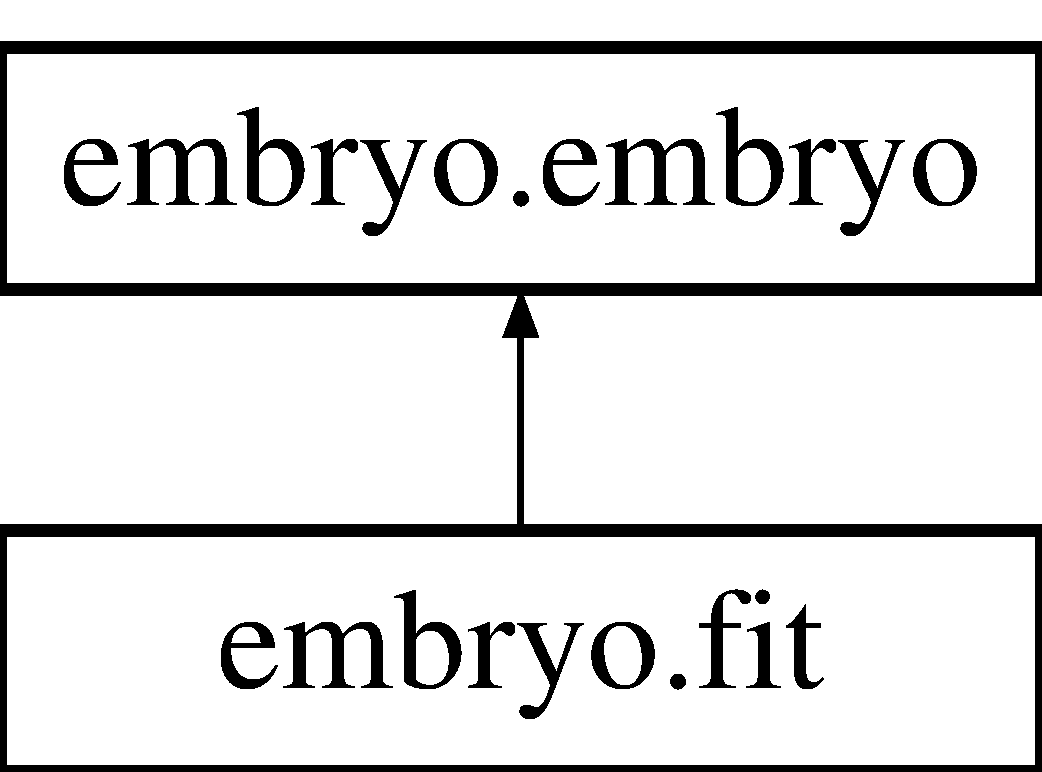
\includegraphics[height=2.000000cm]{classembryo_1_1embryo}
\end{center}
\end{figure}
\subsection*{Public Member Functions}
\begin{DoxyCompactItemize}
\item 
\hypertarget{classembryo_1_1embryo_a8c9736e06943eea20e74b4e25d756e13}{def {\bfseries \+\_\+\+\_\+init\+\_\+\+\_\+}}\label{classembryo_1_1embryo_a8c9736e06943eea20e74b4e25d756e13}

\item 
\hypertarget{classembryo_1_1embryo_aa71724b2ec914d05d54b14e56098e61e}{def {\bfseries add\+\_\+fit}}\label{classembryo_1_1embryo_aa71724b2ec914d05d54b14e56098e61e}

\item 
\hypertarget{classembryo_1_1embryo_a8b50dcd5b39f71114fb69d44481cb70f}{def {\bfseries delete\+\_\+fit}}\label{classembryo_1_1embryo_a8b50dcd5b39f71114fb69d44481cb70f}

\item 
\hypertarget{classembryo_1_1embryo_aaba3a8802e16a4c3f8a5f180cc19e0c2}{def {\bfseries save\+\_\+embryo}}\label{classembryo_1_1embryo_aaba3a8802e16a4c3f8a5f180cc19e0c2}

\item 
\hypertarget{classembryo_1_1embryo_a05834667f02080c3bfb8ba384f881dac}{def {\bfseries load\+\_\+embryo}}\label{classembryo_1_1embryo_a05834667f02080c3bfb8ba384f881dac}

\item 
\hypertarget{classembryo_1_1embryo_a98ae93640d31c33028a6878ae582af3c}{def {\bfseries copy\+\_\+embryo}}\label{classembryo_1_1embryo_a98ae93640d31c33028a6878ae582af3c}

\item 
\hypertarget{classembryo_1_1embryo_af072b0a2ceb5f4b5a93ea8e9c67eabab}{def {\bfseries plot\+\_\+sim\+\_\+data}}\label{classembryo_1_1embryo_af072b0a2ceb5f4b5a93ea8e9c67eabab}

\item 
\hypertarget{classembryo_1_1embryo_a5c224095aa2cf3b212cc9065579be0ee}{def {\bfseries plot\+\_\+sim}}\label{classembryo_1_1embryo_a5c224095aa2cf3b212cc9065579be0ee}

\item 
\hypertarget{classembryo_1_1embryo_a17341daad9b3f77786f11dc815973e73}{def {\bfseries plot\+\_\+data}}\label{classembryo_1_1embryo_a17341daad9b3f77786f11dc815973e73}

\item 
\hypertarget{classembryo_1_1embryo_a37e80c2f0f215104b4d0de83c2afdbee}{def {\bfseries plot\+\_\+pinned}}\label{classembryo_1_1embryo_a37e80c2f0f215104b4d0de83c2afdbee}

\item 
\hypertarget{classembryo_1_1embryo_a645c54f118457a47e2021f3c23382bf3}{def {\bfseries print\+\_\+embryo}}\label{classembryo_1_1embryo_a645c54f118457a47e2021f3c23382bf3}

\item 
\hypertarget{classembryo_1_1embryo_a11846270bbb204206066b911b553e009}{def {\bfseries plot\+\_\+\+I\+C\+\_\+img}}\label{classembryo_1_1embryo_a11846270bbb204206066b911b553e009}

\end{DoxyCompactItemize}
\subsection*{Public Attributes}
\begin{DoxyCompactItemize}
\item 
\hypertarget{classembryo_1_1embryo_ae0ebbb6526872fa3aee3952dc0771922}{{\bfseries name}}\label{classembryo_1_1embryo_ae0ebbb6526872fa3aee3952dc0771922}

\item 
\hypertarget{classembryo_1_1embryo_acee54c01125eaf9802ed9093f4b3512f}{{\bfseries mode}}\label{classembryo_1_1embryo_acee54c01125eaf9802ed9093f4b3512f}

\item 
\hypertarget{classembryo_1_1embryo_a124a831438d741e0f6be09e565162f36}{{\bfseries dataset}}\label{classembryo_1_1embryo_a124a831438d741e0f6be09e565162f36}

\item 
\hypertarget{classembryo_1_1embryo_adb0457d25719622ccdc97f9f6108d704}{{\bfseries emb}}\label{classembryo_1_1embryo_adb0457d25719622ccdc97f9f6108d704}

\item 
\hypertarget{classembryo_1_1embryo_a1e01afc292f74dfe1715609c17aceb22}{{\bfseries fn\+\_\+datafolder}}\label{classembryo_1_1embryo_a1e01afc292f74dfe1715609c17aceb22}

\item 
\hypertarget{classembryo_1_1embryo_affa16779dede9272ca3aade47f26d159}{{\bfseries fn\+\_\+preimage}}\label{classembryo_1_1embryo_affa16779dede9272ca3aade47f26d159}

\item 
\hypertarget{classembryo_1_1embryo_aa726846d41df92feebbe1f0d2fa7d0fa}{{\bfseries fn\+\_\+resultfolder}}\label{classembryo_1_1embryo_aa726846d41df92feebbe1f0d2fa7d0fa}

\item 
\hypertarget{classembryo_1_1embryo_a8b0ff0f47e5134fd764d3a846874cb67}{{\bfseries data\+\_\+enc}}\label{classembryo_1_1embryo_a8b0ff0f47e5134fd764d3a846874cb67}

\item 
\hypertarget{classembryo_1_1embryo_a73b7190c473acfc18b62beacca67c766}{{\bfseries data\+\_\+ft}}\label{classembryo_1_1embryo_a73b7190c473acfc18b62beacca67c766}

\item 
\hypertarget{classembryo_1_1embryo_a280a987c093b60ccb6af5f86b01bb6b0}{{\bfseries data\+\_\+res\+\_\+px}}\label{classembryo_1_1embryo_a280a987c093b60ccb6af5f86b01bb6b0}

\item 
\hypertarget{classembryo_1_1embryo_ad8e234353c366181459b612885245e10}{{\bfseries conv\+\_\+fact}}\label{classembryo_1_1embryo_ad8e234353c366181459b612885245e10}

\item 
\hypertarget{classembryo_1_1embryo_afc58db88e819ee795d262c16b9166c19}{{\bfseries framerate}}\label{classembryo_1_1embryo_afc58db88e819ee795d262c16b9166c19}

\item 
\hypertarget{classembryo_1_1embryo_a0d4cb0531623488d5dba15576170e603}{{\bfseries nframes}}\label{classembryo_1_1embryo_a0d4cb0531623488d5dba15576170e603}

\item 
\hypertarget{classembryo_1_1embryo_a45e2e29b72aa211ccf5147852e241e96}{{\bfseries tstart}}\label{classembryo_1_1embryo_a45e2e29b72aa211ccf5147852e241e96}

\item 
\hypertarget{classembryo_1_1embryo_a8b98cda65ad39c1e3dd83b46644903ab}{{\bfseries tend}}\label{classembryo_1_1embryo_a8b98cda65ad39c1e3dd83b46644903ab}

\item 
\hypertarget{classembryo_1_1embryo_a4a3e15b69fe1355d91867b5447a61641}{{\bfseries tvec\+\_\+data}}\label{classembryo_1_1embryo_a4a3e15b69fe1355d91867b5447a61641}

\item 
\hypertarget{classembryo_1_1embryo_ae098d9ddbfe187a09316027fb6c71342}{{\bfseries steps\+\_\+data}}\label{classembryo_1_1embryo_ae098d9ddbfe187a09316027fb6c71342}

\item 
\hypertarget{classembryo_1_1embryo_adbbe9beb8e1283419375a8307f7b68d9}{{\bfseries dt\+\_\+data}}\label{classembryo_1_1embryo_adbbe9beb8e1283419375a8307f7b68d9}

\item 
\hypertarget{classembryo_1_1embryo_a863ca8dc0a22a2d83a14b4762f732495}{{\bfseries side\+\_\+length\+\_\+bleached\+\_\+mu}}\label{classembryo_1_1embryo_a863ca8dc0a22a2d83a14b4762f732495}

\item 
\hypertarget{classembryo_1_1embryo_a78560ec7cc5326de307eb48dd0617317}{{\bfseries fish\+\_\+outradius\+\_\+mu}}\label{classembryo_1_1embryo_a78560ec7cc5326de307eb48dd0617317}

\item 
\hypertarget{classembryo_1_1embryo_a497b17913f59268b561fa4681d74918e}{{\bfseries slice\+\_\+depth\+\_\+mu}}\label{classembryo_1_1embryo_a497b17913f59268b561fa4681d74918e}

\item 
\hypertarget{classembryo_1_1embryo_a9ae5d9370dd9e435df0db60ae58d94a4}{{\bfseries radius\+\_\+embr\+\_\+mu}}\label{classembryo_1_1embryo_a9ae5d9370dd9e435df0db60ae58d94a4}

\item 
\hypertarget{classembryo_1_1embryo_a08a439e8e3a51402be2f468497443424}{{\bfseries slice\+\_\+width\+\_\+mu}}\label{classembryo_1_1embryo_a08a439e8e3a51402be2f468497443424}

\item 
\hypertarget{classembryo_1_1embryo_a50af89511d9959240f4a3c3fd1331e54}{{\bfseries cylinder\+\_\+radius\+\_\+mu}}\label{classembryo_1_1embryo_a50af89511d9959240f4a3c3fd1331e54}

\item 
\hypertarget{classembryo_1_1embryo_abba4f6d3ba47dfb7cd2632d27a1fb4d3}{{\bfseries cylinder\+\_\+height\+\_\+mu}}\label{classembryo_1_1embryo_abba4f6d3ba47dfb7cd2632d27a1fb4d3}

\item 
\hypertarget{classembryo_1_1embryo_a1628c3105fc55d5ceb3c340390147ad0}{{\bfseries frog\+\_\+radius\+\_\+mu}}\label{classembryo_1_1embryo_a1628c3105fc55d5ceb3c340390147ad0}

\item 
\hypertarget{classembryo_1_1embryo_acb9fdadefd3e07c209e0746f78e6b583}{{\bfseries slice\+\_\+width\+\_\+px}}\label{classembryo_1_1embryo_acb9fdadefd3e07c209e0746f78e6b583}

\item 
\hypertarget{classembryo_1_1embryo_aaec6e88ef25fabf76e1d77f5ce6100e4}{{\bfseries slice\+\_\+depth\+\_\+px}}\label{classembryo_1_1embryo_aaec6e88ef25fabf76e1d77f5ce6100e4}

\item 
\hypertarget{classembryo_1_1embryo_a5192437f219867f92442306e68ff631f}{{\bfseries slice\+\_\+height\+\_\+px}}\label{classembryo_1_1embryo_a5192437f219867f92442306e68ff631f}

\item 
\hypertarget{classembryo_1_1embryo_a6c23d8c0af90025172a106598b6e0b36}{{\bfseries slice\+\_\+bottom}}\label{classembryo_1_1embryo_a6c23d8c0af90025172a106598b6e0b36}

\item 
\hypertarget{classembryo_1_1embryo_a5ef1f4393b163fbbdf30f4a354123d8c}{{\bfseries center\+\_\+embr\+\_\+px}}\label{classembryo_1_1embryo_a5ef1f4393b163fbbdf30f4a354123d8c}

\item 
\hypertarget{classembryo_1_1embryo_ac6d7dee4903057522d3f3709f2304797}{{\bfseries side\+\_\+length\+\_\+bleached\+\_\+px}}\label{classembryo_1_1embryo_ac6d7dee4903057522d3f3709f2304797}

\item 
\hypertarget{classembryo_1_1embryo_aa1469f877e3e276f6f73692af3ffaf5d}{{\bfseries offset\+\_\+bleached\+\_\+px}}\label{classembryo_1_1embryo_aa1469f877e3e276f6f73692af3ffaf5d}

\item 
\hypertarget{classembryo_1_1embryo_a0369d96c13c2ed1efd52acb621901aac}{{\bfseries radius\+\_\+embr\+\_\+px}}\label{classembryo_1_1embryo_a0369d96c13c2ed1efd52acb621901aac}

\item 
\hypertarget{classembryo_1_1embryo_a03b94de470e57b71e62b750245051514}{{\bfseries man\+\_\+det}}\label{classembryo_1_1embryo_a03b94de470e57b71e62b750245051514}

\item 
\hypertarget{classembryo_1_1embryo_a08e582f4c78ce2488753dd699bf4f49d}{{\bfseries auto\+\_\+det}}\label{classembryo_1_1embryo_a08e582f4c78ce2488753dd699bf4f49d}

\item 
\hypertarget{classembryo_1_1embryo_acc333ed7a2f594ce2e539170d6ecdc53}{{\bfseries parms\+\_\+det}}\label{classembryo_1_1embryo_acc333ed7a2f594ce2e539170d6ecdc53}

\item 
\hypertarget{classembryo_1_1embryo_a2dbd78a0b04482bd7abe321969e23c5e}{{\bfseries gauss\+\_\+opt}}\label{classembryo_1_1embryo_a2dbd78a0b04482bd7abe321969e23c5e}

\item 
\hypertarget{classembryo_1_1embryo_a373ce3af19856c2a94bb9db8ae3d62d9}{{\bfseries surf\+\_\+opt}}\label{classembryo_1_1embryo_a373ce3af19856c2a94bb9db8ae3d62d9}

\item 
\hypertarget{classembryo_1_1embryo_ad50942537943f3dda8997c5097562019}{{\bfseries add\+\_\+rim\+\_\+img}}\label{classembryo_1_1embryo_ad50942537943f3dda8997c5097562019}

\item 
\hypertarget{classembryo_1_1embryo_a31eff41fc404117e1f994c0f77ccfca8}{{\bfseries squ\+\_\+av\+\_\+data\+\_\+d}}\label{classembryo_1_1embryo_a31eff41fc404117e1f994c0f77ccfca8}

\item 
\hypertarget{classembryo_1_1embryo_a409acdd8a25a99b1d9c076a8bd17566f}{{\bfseries out\+\_\+av\+\_\+data\+\_\+d}}\label{classembryo_1_1embryo_a409acdd8a25a99b1d9c076a8bd17566f}

\item 
\hypertarget{classembryo_1_1embryo_af70f2bdd69e4f990d2884b2dcaa4dfdc}{{\bfseries slice\+\_\+av\+\_\+data\+\_\+d}}\label{classembryo_1_1embryo_af70f2bdd69e4f990d2884b2dcaa4dfdc}

\item 
\hypertarget{classembryo_1_1embryo_a9d18b75d3da73770c640e711e3cf3a28}{{\bfseries im\+\_\+reg\+\_\+\+I\+Cs}}\label{classembryo_1_1embryo_a9d18b75d3da73770c640e711e3cf3a28}

\item 
\hypertarget{classembryo_1_1embryo_ade854551852366b822389cf191d120b9}{{\bfseries rim}}\label{classembryo_1_1embryo_ade854551852366b822389cf191d120b9}

\item 
\hypertarget{classembryo_1_1embryo_a38f1cf7467c55ae5ce8fb7dd32482314}{{\bfseries debug\+\_\+analysis}}\label{classembryo_1_1embryo_a38f1cf7467c55ae5ce8fb7dd32482314}

\item 
\hypertarget{classembryo_1_1embryo_aff9707595de111dcdfdcb7ef1830d00e}{{\bfseries add\+\_\+rim\+\_\+from\+\_\+radius}}\label{classembryo_1_1embryo_aff9707595de111dcdfdcb7ef1830d00e}

\item 
\hypertarget{classembryo_1_1embryo_a26dd617076f8217bbc5ea7d3f3cff80b}{{\bfseries conc\+\_\+rim}}\label{classembryo_1_1embryo_a26dd617076f8217bbc5ea7d3f3cff80b}

\item 
\hypertarget{classembryo_1_1embryo_af1008dee112ecd61ffb385a46dee51d9}{{\bfseries img\+\_\+in\+\_\+domain}}\label{classembryo_1_1embryo_af1008dee112ecd61ffb385a46dee51d9}

\item 
\hypertarget{classembryo_1_1embryo_a3ec820560f121e70c2bde477b253ccee}{{\bfseries norm\+\_\+by\+\_\+pre}}\label{classembryo_1_1embryo_a3ec820560f121e70c2bde477b253ccee}

\item 
\hypertarget{classembryo_1_1embryo_a49716349d5505e72ca46ad8bffcc109b}{{\bfseries phi\+\_\+\+I\+C\+\_\+rad}}\label{classembryo_1_1embryo_a49716349d5505e72ca46ad8bffcc109b}

\item 
\hypertarget{classembryo_1_1embryo_a6a6cd2baa4ca0bc7ab3bbbca06dbb426}{{\bfseries phi\+\_\+\+I\+C\+\_\+rad\+\_\+mesh}}\label{classembryo_1_1embryo_a6a6cd2baa4ca0bc7ab3bbbca06dbb426}

\item 
\hypertarget{classembryo_1_1embryo_a8d18dae0b04d38e0d9cf61ce39cac4f3}{{\bfseries rad\+\_\+steps}}\label{classembryo_1_1embryo_a8d18dae0b04d38e0d9cf61ce39cac4f3}

\item 
\hypertarget{classembryo_1_1embryo_ad23e4601d53381edfede320d59181829}{{\bfseries phi\+\_\+\+I\+C\+\_\+bleached}}\label{classembryo_1_1embryo_ad23e4601d53381edfede320d59181829}

\item 
\hypertarget{classembryo_1_1embryo_a2d73df502e4a1779636627ac3d1a7ed9}{{\bfseries debug\+\_\+preproc}}\label{classembryo_1_1embryo_a2d73df502e4a1779636627ac3d1a7ed9}

\item 
\hypertarget{classembryo_1_1embryo_aeb420310bf647abe3e7e3b50a1c5ce01}{{\bfseries rad\+\_\+step\+\_\+px}}\label{classembryo_1_1embryo_aeb420310bf647abe3e7e3b50a1c5ce01}

\item 
\hypertarget{classembryo_1_1embryo_a8a8d0d4c9d72ebf0e434eb76c0ec13b1}{{\bfseries geometry}}\label{classembryo_1_1embryo_a8a8d0d4c9d72ebf0e434eb76c0ec13b1}

\item 
\hypertarget{classembryo_1_1embryo_ae74cd3b7d7515e9ed76fc1379465cc4f}{{\bfseries fish\+\_\+outradius\+\_\+px}}\label{classembryo_1_1embryo_ae74cd3b7d7515e9ed76fc1379465cc4f}

\item 
\hypertarget{classembryo_1_1embryo_a275eb02ac6bce7c9a4c1cc743d77d5a3}{{\bfseries fish\+\_\+inradius\+\_\+px}}\label{classembryo_1_1embryo_a275eb02ac6bce7c9a4c1cc743d77d5a3}

\item 
\hypertarget{classembryo_1_1embryo_ab74886b9fc29d3151641875e3d272fe1}{{\bfseries fish\+\_\+dist\+\_\+px}}\label{classembryo_1_1embryo_ab74886b9fc29d3151641875e3d272fe1}

\item 
\hypertarget{classembryo_1_1embryo_a6aed3fc750d6383e709950a47bd34e26}{{\bfseries frog\+\_\+radius\+\_\+px}}\label{classembryo_1_1embryo_a6aed3fc750d6383e709950a47bd34e26}

\item 
\hypertarget{classembryo_1_1embryo_ada8df0c4602a49b3716a10ee4ecbc19e}{{\bfseries cylinder\+\_\+radius\+\_\+px}}\label{classembryo_1_1embryo_ada8df0c4602a49b3716a10ee4ecbc19e}

\item 
\hypertarget{classembryo_1_1embryo_a26c0a7a0e3c58fcf41084f3f4d8676d3}{{\bfseries cylinder\+\_\+height\+\_\+px}}\label{classembryo_1_1embryo_a26c0a7a0e3c58fcf41084f3f4d8676d3}

\item 
\hypertarget{classembryo_1_1embryo_a25155e89a8b14ad4c13dd360a65354db}{{\bfseries apply\+\_\+data}}\label{classembryo_1_1embryo_a25155e89a8b14ad4c13dd360a65354db}

\item 
\hypertarget{classembryo_1_1embryo_aefc1a4e6b46f71d3ce5579e3860be807}{{\bfseries D}}\label{classembryo_1_1embryo_aefc1a4e6b46f71d3ce5579e3860be807}

\item 
\hypertarget{classembryo_1_1embryo_aa29a0618bf04c643dd485a4e26df0268}{{\bfseries prod}}\label{classembryo_1_1embryo_aa29a0618bf04c643dd485a4e26df0268}

\item 
\hypertarget{classembryo_1_1embryo_abd16a13c0a0e9f4d91f73744c6e9dcb3}{{\bfseries degr}}\label{classembryo_1_1embryo_abd16a13c0a0e9f4d91f73744c6e9dcb3}

\item 
\hypertarget{classembryo_1_1embryo_a216b686732f6d4f7ade516fd53e6d979}{{\bfseries steps\+\_\+sim}}\label{classembryo_1_1embryo_a216b686732f6d4f7ade516fd53e6d979}

\item 
\hypertarget{classembryo_1_1embryo_ac1085d360070f463a85609a9ea75d378}{{\bfseries tvec\+\_\+sim}}\label{classembryo_1_1embryo_ac1085d360070f463a85609a9ea75d378}

\item 
\hypertarget{classembryo_1_1embryo_ad6651c224a634ef15efaae0b60eae897}{{\bfseries avg\+\_\+mode}}\label{classembryo_1_1embryo_ad6651c224a634ef15efaae0b60eae897}

\item 
\hypertarget{classembryo_1_1embryo_ad6d67eaa26312172b343c9f656875ea7}{{\bfseries add\+\_\+rim\+\_\+sim}}\label{classembryo_1_1embryo_ad6d67eaa26312172b343c9f656875ea7}

\item 
\hypertarget{classembryo_1_1embryo_afab8d189c45ff7ad5e94b84f92e3319b}{{\bfseries avg\+\_\+outer}}\label{classembryo_1_1embryo_afab8d189c45ff7ad5e94b84f92e3319b}

\item 
\hypertarget{classembryo_1_1embryo_a9194f2535a1a9a3b8e8650b21251d5ca}{{\bfseries avg\+\_\+inner}}\label{classembryo_1_1embryo_a9194f2535a1a9a3b8e8650b21251d5ca}

\item 
\hypertarget{classembryo_1_1embryo_aba840a41d4f78139c2d85a03b489172d}{{\bfseries avg\+\_\+all}}\label{classembryo_1_1embryo_aba840a41d4f78139c2d85a03b489172d}

\item 
\hypertarget{classembryo_1_1embryo_ae843c1e621c611d643f0f860822ab0c1}{{\bfseries avg\+\_\+pocket}}\label{classembryo_1_1embryo_ae843c1e621c611d643f0f860822ab0c1}

\item 
\hypertarget{classembryo_1_1embryo_a40b4792398fd63cc5acd8a0fbfd58d63}{{\bfseries avg\+\_\+small}}\label{classembryo_1_1embryo_a40b4792398fd63cc5acd8a0fbfd58d63}

\item 
\hypertarget{classembryo_1_1embryo_a8391f006bba7ec7f7bfffa87fcfbe9e1}{{\bfseries squ\+\_\+av\+\_\+d}}\label{classembryo_1_1embryo_a8391f006bba7ec7f7bfffa87fcfbe9e1}

\item 
\hypertarget{classembryo_1_1embryo_a8a868d80a4415f21a42b8cc4eece0115}{{\bfseries out\+\_\+av\+\_\+d}}\label{classembryo_1_1embryo_a8a868d80a4415f21a42b8cc4eece0115}

\item 
\hypertarget{classembryo_1_1embryo_ac6835656a266d4de59b7f719aa3109c3}{{\bfseries slice\+\_\+av\+\_\+d}}\label{classembryo_1_1embryo_ac6835656a266d4de59b7f719aa3109c3}

\item 
\hypertarget{classembryo_1_1embryo_a56b5eee866284e5ab34d21ad46b7202f}{{\bfseries inner\+\_\+av\+\_\+d}}\label{classembryo_1_1embryo_a56b5eee866284e5ab34d21ad46b7202f}

\item 
\hypertarget{classembryo_1_1embryo_a5bce0cd1ce424e45c23bf6283620cca7}{{\bfseries outer\+\_\+av\+\_\+d}}\label{classembryo_1_1embryo_a5bce0cd1ce424e45c23bf6283620cca7}

\item 
\hypertarget{classembryo_1_1embryo_a9e0e098fc9faf4dcba041c16c3db6572}{{\bfseries squ\+\_\+pocket\+\_\+av\+\_\+d}}\label{classembryo_1_1embryo_a9e0e098fc9faf4dcba041c16c3db6572}

\item 
\hypertarget{classembryo_1_1embryo_a3ef889edffc28fbae112e3795db6511b}{{\bfseries out\+\_\+pocket\+\_\+av\+\_\+d}}\label{classembryo_1_1embryo_a3ef889edffc28fbae112e3795db6511b}

\item 
\hypertarget{classembryo_1_1embryo_a7ccec2ef95acb7a5d02039310623f2d5}{{\bfseries squ\+\_\+small\+\_\+av\+\_\+d}}\label{classembryo_1_1embryo_a7ccec2ef95acb7a5d02039310623f2d5}

\item 
\hypertarget{classembryo_1_1embryo_a01c596c10965827f899fe6e58dfa656b}{{\bfseries out\+\_\+small\+\_\+av\+\_\+d}}\label{classembryo_1_1embryo_a01c596c10965827f899fe6e58dfa656b}

\item 
\hypertarget{classembryo_1_1embryo_aff49aa118824f13fc53ebf4744f36a57}{{\bfseries all\+\_\+av\+\_\+d}}\label{classembryo_1_1embryo_aff49aa118824f13fc53ebf4744f36a57}

\item 
\hypertarget{classembryo_1_1embryo_a7da9fe408f9bac60e8590ee16df21cfd}{{\bfseries vol\+Size\+\_\+px}}\label{classembryo_1_1embryo_a7da9fe408f9bac60e8590ee16df21cfd}

\item 
\hypertarget{classembryo_1_1embryo_a7a3d14fe04b138097cad553e7c0e2b6f}{{\bfseries fn\+\_\+mesh}}\label{classembryo_1_1embryo_a7a3d14fe04b138097cad553e7c0e2b6f}

\item 
\hypertarget{classembryo_1_1embryo_a6b8f9eb83227c6a4d8769950e1c76380}{{\bfseries debug\+\_\+simulation}}\label{classembryo_1_1embryo_a6b8f9eb83227c6a4d8769950e1c76380}

\item 
\hypertarget{classembryo_1_1embryo_a6c986b486222617146705ac397c803ab}{{\bfseries mesh}}\label{classembryo_1_1embryo_a6c986b486222617146705ac397c803ab}

\item 
\hypertarget{classembryo_1_1embryo_a82ba7affcc8eea4554d3aaf0be28e971}{{\bfseries usemesh}}\label{classembryo_1_1embryo_a82ba7affcc8eea4554d3aaf0be28e971}

\item 
\hypertarget{classembryo_1_1embryo_afd270cee2465b7fc73c333a9a4cbebc0}{{\bfseries usemap}}\label{classembryo_1_1embryo_afd270cee2465b7fc73c333a9a4cbebc0}

\item 
\hypertarget{classembryo_1_1embryo_a006d63493b2c1b657eacfc46d2c8522b}{{\bfseries mesh\+\_\+maps}}\label{classembryo_1_1embryo_a006d63493b2c1b657eacfc46d2c8522b}

\item 
\hypertarget{classembryo_1_1embryo_a6c6e8a7e5df9cc4ba11a2b15c0e0ed34}{{\bfseries optim}}\label{classembryo_1_1embryo_a6c6e8a7e5df9cc4ba11a2b15c0e0ed34}

\item 
\hypertarget{classembryo_1_1embryo_a26c812c2165b6f8fc465d3d05ac05f22}{{\bfseries int\+\_\+steps}}\label{classembryo_1_1embryo_a26c812c2165b6f8fc465d3d05ac05f22}

\item 
\hypertarget{classembryo_1_1embryo_a405e918222a70357db62cb80c65578a2}{{\bfseries integration\+\_\+method}}\label{classembryo_1_1embryo_a405e918222a70357db62cb80c65578a2}

\item 
\hypertarget{classembryo_1_1embryo_a5808ed9d1e5321d7b4b2536256fbf908}{{\bfseries reg\+\_\+mesh\+\_\+opt}}\label{classembryo_1_1embryo_a5808ed9d1e5321d7b4b2536256fbf908}

\item 
\hypertarget{classembryo_1_1embryo_a4ee68ad592d1c32ce5017c78edcec427}{{\bfseries res\+\_\+reg}}\label{classembryo_1_1embryo_a4ee68ad592d1c32ce5017c78edcec427}

\item 
\hypertarget{classembryo_1_1embryo_a169ddb8497d34e77066b4c5366e45c7a}{{\bfseries res\+\_\+wire}}\label{classembryo_1_1embryo_a169ddb8497d34e77066b4c5366e45c7a}

\item 
\hypertarget{classembryo_1_1embryo_a17899b807c4b94adb6684c8db91c0d7e}{{\bfseries debug\+\_\+reg}}\label{classembryo_1_1embryo_a17899b807c4b94adb6684c8db91c0d7e}

\item 
\hypertarget{classembryo_1_1embryo_acc2469130b47222b979fd3b653296b22}{{\bfseries mask\+\_\+squ}}\label{classembryo_1_1embryo_acc2469130b47222b979fd3b653296b22}

\item 
\hypertarget{classembryo_1_1embryo_a2215ce9969d0023ae6087b0b5e60c29b}{{\bfseries mask\+\_\+out}}\label{classembryo_1_1embryo_a2215ce9969d0023ae6087b0b5e60c29b}

\item 
\hypertarget{classembryo_1_1embryo_a7904d811970aa50493d52c9b8a53aca2}{{\bfseries mask\+\_\+slice}}\label{classembryo_1_1embryo_a7904d811970aa50493d52c9b8a53aca2}

\item 
\hypertarget{classembryo_1_1embryo_a71f0cb4f04101442306d9dc8f1af17dc}{{\bfseries plot\+\_\+wire}}\label{classembryo_1_1embryo_a71f0cb4f04101442306d9dc8f1af17dc}

\item 
\hypertarget{classembryo_1_1embryo_a922028622d8b4b8aabdf06ca112b4922}{{\bfseries plot\+\_\+cont}}\label{classembryo_1_1embryo_a922028622d8b4b8aabdf06ca112b4922}

\item 
\hypertarget{classembryo_1_1embryo_acdb9af330d4b8cf8fbbf4a94b6b97212}{{\bfseries plot\+\_\+conc}}\label{classembryo_1_1embryo_acdb9af330d4b8cf8fbbf4a94b6b97212}

\item 
\hypertarget{classembryo_1_1embryo_a2577e63908916a69db66975e84c15436}{{\bfseries plot\+\_\+surf}}\label{classembryo_1_1embryo_a2577e63908916a69db66975e84c15436}

\item 
\hypertarget{classembryo_1_1embryo_a29368d21e8573c2932dc1cb0ce29c469}{{\bfseries plot\+\_\+all}}\label{classembryo_1_1embryo_a29368d21e8573c2932dc1cb0ce29c469}

\item 
\hypertarget{classembryo_1_1embryo_a5facb157131fad6e9be0176dcd705f7a}{{\bfseries out\+\_\+wire}}\label{classembryo_1_1embryo_a5facb157131fad6e9be0176dcd705f7a}

\item 
\hypertarget{classembryo_1_1embryo_a2313d46c5a0ca4afbd07c30f8a2f5087}{{\bfseries out\+\_\+cont}}\label{classembryo_1_1embryo_a2313d46c5a0ca4afbd07c30f8a2f5087}

\item 
\hypertarget{classembryo_1_1embryo_ae219eab430fe485898080ad0ecf1e89d}{{\bfseries out\+\_\+conc}}\label{classembryo_1_1embryo_ae219eab430fe485898080ad0ecf1e89d}

\item 
\hypertarget{classembryo_1_1embryo_aa95072fe1c601c6c801f584b946d5e33}{{\bfseries out\+\_\+surf}}\label{classembryo_1_1embryo_aa95072fe1c601c6c801f584b946d5e33}

\item 
\hypertarget{classembryo_1_1embryo_a4fc7e65cbed79c3bb8827db5929e0c4c}{{\bfseries out\+\_\+all}}\label{classembryo_1_1embryo_a4fc7e65cbed79c3bb8827db5929e0c4c}

\item 
\hypertarget{classembryo_1_1embryo_ae98d721268c8d9d51b3542fea917864c}{{\bfseries squ\+\_\+av\+\_\+pm\+\_\+d}}\label{classembryo_1_1embryo_ae98d721268c8d9d51b3542fea917864c}

\item 
\hypertarget{classembryo_1_1embryo_a7d1fbde1a4aceeba9d7b10900a3205bf}{{\bfseries out\+\_\+av\+\_\+pm\+\_\+d}}\label{classembryo_1_1embryo_a7d1fbde1a4aceeba9d7b10900a3205bf}

\item 
\hypertarget{classembryo_1_1embryo_a0439d5d56f696fff851b1d30f6bf5db1}{{\bfseries slice\+\_\+av\+\_\+pm\+\_\+d}}\label{classembryo_1_1embryo_a0439d5d56f696fff851b1d30f6bf5db1}

\item 
\hypertarget{classembryo_1_1embryo_a867c4a808ae1e165c3c2d96340531d19}{{\bfseries inner\+\_\+av\+\_\+pm\+\_\+d}}\label{classembryo_1_1embryo_a867c4a808ae1e165c3c2d96340531d19}

\item 
\hypertarget{classembryo_1_1embryo_abed079f70482ee69ac10ef22f06a3a50}{{\bfseries outer\+\_\+av\+\_\+pm\+\_\+d}}\label{classembryo_1_1embryo_abed079f70482ee69ac10ef22f06a3a50}

\item 
\hypertarget{classembryo_1_1embryo_a69b08f42bea20bf1135eeada41a24026}{{\bfseries all\+\_\+av\+\_\+pm\+\_\+d}}\label{classembryo_1_1embryo_a69b08f42bea20bf1135eeada41a24026}

\item 
\hypertarget{classembryo_1_1embryo_abc22229e40802080b85c0f79692e60a5}{{\bfseries squ\+\_\+pocket\+\_\+av\+\_\+pm\+\_\+d}}\label{classembryo_1_1embryo_abc22229e40802080b85c0f79692e60a5}

\item 
\hypertarget{classembryo_1_1embryo_ab193be7b547053d90eddfe30aaeffba7}{{\bfseries out\+\_\+pocket\+\_\+av\+\_\+pm\+\_\+d}}\label{classembryo_1_1embryo_ab193be7b547053d90eddfe30aaeffba7}

\item 
\hypertarget{classembryo_1_1embryo_a7abb0db73b591dcee46213bb93d71315}{{\bfseries squ\+\_\+small\+\_\+av\+\_\+pm\+\_\+d}}\label{classembryo_1_1embryo_a7abb0db73b591dcee46213bb93d71315}

\item 
\hypertarget{classembryo_1_1embryo_a119bc7d2e2e726522464b61536394f9d}{{\bfseries out\+\_\+small\+\_\+av\+\_\+pm\+\_\+d}}\label{classembryo_1_1embryo_a119bc7d2e2e726522464b61536394f9d}

\item 
\hypertarget{classembryo_1_1embryo_ae184171cbf20148bbe21664d78c49855}{{\bfseries debug\+\_\+pinning}}\label{classembryo_1_1embryo_ae184171cbf20148bbe21664d78c49855}

\item 
\hypertarget{classembryo_1_1embryo_a531c36fe2c9047a75349df1878b9def6}{{\bfseries squ\+\_\+av\+\_\+pinned\+\_\+d}}\label{classembryo_1_1embryo_a531c36fe2c9047a75349df1878b9def6}

\item 
\hypertarget{classembryo_1_1embryo_a65e27ced4e50dce639c8bc3e37557e52}{{\bfseries out\+\_\+av\+\_\+pinned\+\_\+d}}\label{classembryo_1_1embryo_a65e27ced4e50dce639c8bc3e37557e52}

\item 
\hypertarget{classembryo_1_1embryo_a3f8349338ddeafc0849e5500e0067dbe}{{\bfseries slice\+\_\+av\+\_\+pinned\+\_\+d}}\label{classembryo_1_1embryo_a3f8349338ddeafc0849e5500e0067dbe}

\item 
\hypertarget{classembryo_1_1embryo_a665ee53ff14d5b47b742cf8c76c37e08}{{\bfseries inner\+\_\+av\+\_\+pinned\+\_\+d}}\label{classembryo_1_1embryo_a665ee53ff14d5b47b742cf8c76c37e08}

\item 
\hypertarget{classembryo_1_1embryo_ad3f4d22c3fba9f704210cf38c724fb21}{{\bfseries outer\+\_\+av\+\_\+pinned\+\_\+d}}\label{classembryo_1_1embryo_ad3f4d22c3fba9f704210cf38c724fb21}

\item 
\hypertarget{classembryo_1_1embryo_aaea0743a4a39beee257eafbbddb4291a}{{\bfseries squ\+\_\+pocket\+\_\+av\+\_\+pinned\+\_\+d}}\label{classembryo_1_1embryo_aaea0743a4a39beee257eafbbddb4291a}

\item 
\hypertarget{classembryo_1_1embryo_a6345c7523d7b024caeeb3786220c449b}{{\bfseries out\+\_\+pocket\+\_\+av\+\_\+pinned\+\_\+d}}\label{classembryo_1_1embryo_a6345c7523d7b024caeeb3786220c449b}

\item 
\hypertarget{classembryo_1_1embryo_a5816f5e8546ca09c73dd7d05d2f4a100}{{\bfseries squ\+\_\+small\+\_\+av\+\_\+pinned\+\_\+d}}\label{classembryo_1_1embryo_a5816f5e8546ca09c73dd7d05d2f4a100}

\item 
\hypertarget{classembryo_1_1embryo_adb59c65f52d259c0487742d865f956ca}{{\bfseries out\+\_\+small\+\_\+av\+\_\+pinned\+\_\+d}}\label{classembryo_1_1embryo_adb59c65f52d259c0487742d865f956ca}

\item 
\hypertarget{classembryo_1_1embryo_aea06f3112e743f286ef5c1fcbd893587}{{\bfseries all\+\_\+av\+\_\+pinned\+\_\+d}}\label{classembryo_1_1embryo_aea06f3112e743f286ef5c1fcbd893587}

\item 
\hypertarget{classembryo_1_1embryo_adf576eead3db93f965bff38fe1a18c4b}{{\bfseries squ\+\_\+av\+\_\+data\+\_\+pinned\+\_\+d}}\label{classembryo_1_1embryo_adf576eead3db93f965bff38fe1a18c4b}

\item 
\hypertarget{classembryo_1_1embryo_a64d4d7f0617097676804aa597216b3a9}{{\bfseries out\+\_\+av\+\_\+data\+\_\+pinned\+\_\+d}}\label{classembryo_1_1embryo_a64d4d7f0617097676804aa597216b3a9}

\item 
\hypertarget{classembryo_1_1embryo_a18e49e1c8b4529a3e49939b305f51434}{{\bfseries slice\+\_\+av\+\_\+data\+\_\+pinned\+\_\+d}}\label{classembryo_1_1embryo_a18e49e1c8b4529a3e49939b305f51434}

\item 
\hypertarget{classembryo_1_1embryo_a95c0d980a1f47bd0b676bc6c45559cc8}{{\bfseries fit\+\_\+number}}\label{classembryo_1_1embryo_a95c0d980a1f47bd0b676bc6c45559cc8}

\item 
\hypertarget{classembryo_1_1embryo_a96df10bf6666274a710d367b3cee1c95}{{\bfseries fits}}\label{classembryo_1_1embryo_a96df10bf6666274a710d367b3cee1c95}

\item 
\hypertarget{classembryo_1_1embryo_ac77512e3887e49ca8852f4cbf722d3fd}{{\bfseries debug\+\_\+fit}}\label{classembryo_1_1embryo_ac77512e3887e49ca8852f4cbf722d3fd}

\end{DoxyCompactItemize}


The documentation for this class was generated from the following file\+:\begin{DoxyCompactItemize}
\item 
/home/alex\+\_\+loc/\+Documents/\+Research/\+Py\+F\+R\+A\+P/\+Code/embryo.\+py\end{DoxyCompactItemize}

\hypertarget{classembryo_1_1fit}{\section{embryo.\+fit Class Reference}
\label{classembryo_1_1fit}\index{embryo.\+fit@{embryo.\+fit}}
}
Inheritance diagram for embryo.\+fit\+:\begin{figure}[H]
\begin{center}
\leavevmode
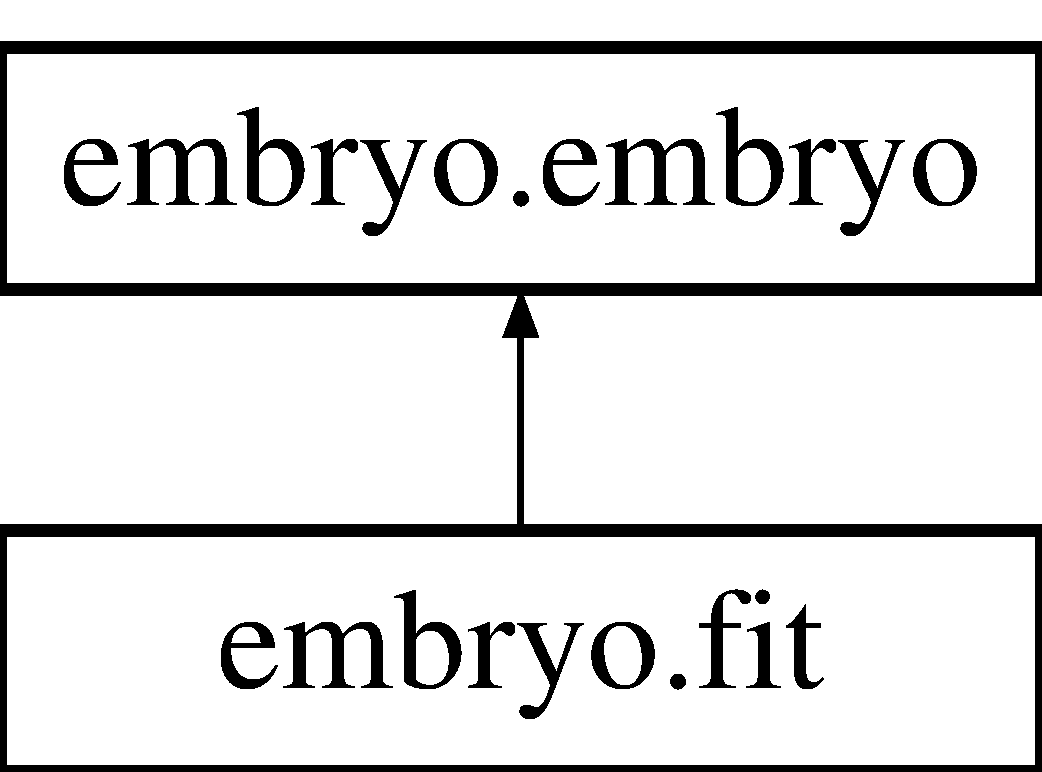
\includegraphics[height=2.000000cm]{classembryo_1_1fit}
\end{center}
\end{figure}
\subsection*{Public Member Functions}
\begin{DoxyCompactItemize}
\item 
\hypertarget{classembryo_1_1fit_aa0928c5edcffbaf495383e1d3e4cbadc}{def {\bfseries \+\_\+\+\_\+init\+\_\+\+\_\+}}\label{classembryo_1_1fit_aa0928c5edcffbaf495383e1d3e4cbadc}

\item 
\hypertarget{classembryo_1_1fit_ab0e8628e65a8a7559c5858cce9e830a8}{def {\bfseries print\+\_\+fit}}\label{classembryo_1_1fit_ab0e8628e65a8a7559c5858cce9e830a8}

\item 
\hypertarget{classembryo_1_1fit_af091775791ed6273b1f32544db3744ac}{def {\bfseries print\+\_\+results}}\label{classembryo_1_1fit_af091775791ed6273b1f32544db3744ac}

\item 
\hypertarget{classembryo_1_1fit_a549bcaa42b6fe95f866e2d9079921dfd}{def {\bfseries plot\+\_\+fit\+\_\+pinned}}\label{classembryo_1_1fit_a549bcaa42b6fe95f866e2d9079921dfd}

\item 
\hypertarget{classembryo_1_1fit_ad013922f972a1c98ce29476eb91deff6}{def {\bfseries plot\+\_\+fit\+\_\+unpinned}}\label{classembryo_1_1fit_ad013922f972a1c98ce29476eb91deff6}

\item 
\hypertarget{classembryo_1_1fit_a2336e12b8a2a2f175f9ea9c75cda7426}{def \hyperlink{classembryo_1_1fit_a2336e12b8a2a2f175f9ea9c75cda7426}{save\+\_\+plot\+\_\+fit\+\_\+pinned}}\label{classembryo_1_1fit_a2336e12b8a2a2f175f9ea9c75cda7426}

\begin{DoxyCompactList}\small\item\em saves plot with simulation and data timeseries \end{DoxyCompactList}\item 
\hypertarget{classembryo_1_1fit_a817798d47a6e35f9680e78e6fae2264d}{def {\bfseries save\+\_\+plot\+\_\+fit\+\_\+unpinned}}\label{classembryo_1_1fit_a817798d47a6e35f9680e78e6fae2264d}

\end{DoxyCompactItemize}
\subsection*{Public Attributes}
\begin{DoxyCompactItemize}
\item 
\hypertarget{classembryo_1_1fit_ab20b4320537edd97bccb47b1b8a32c8c}{{\bfseries fit\+\_\+number}}\label{classembryo_1_1fit_ab20b4320537edd97bccb47b1b8a32c8c}

\item 
\hypertarget{classembryo_1_1fit_a5af0d0f3833064e65ae0a1e8209c8759}{{\bfseries name}}\label{classembryo_1_1fit_a5af0d0f3833064e65ae0a1e8209c8759}

\item 
\hypertarget{classembryo_1_1fit_a3e9f45b92f71ca29744e3d3c02e984f5}{{\bfseries embryo}}\label{classembryo_1_1fit_a3e9f45b92f71ca29744e3d3c02e984f5}

\item 
\hypertarget{classembryo_1_1fit_a9c2c42470cd3dbfb7c3551c446e17a0b}{{\bfseries opt\+\_\+meth}}\label{classembryo_1_1fit_a9c2c42470cd3dbfb7c3551c446e17a0b}

\item 
\hypertarget{classembryo_1_1fit_a740dc4ca6efdae5615848bcd3f0277ba}{{\bfseries fit\+\_\+squ}}\label{classembryo_1_1fit_a740dc4ca6efdae5615848bcd3f0277ba}

\item 
\hypertarget{classembryo_1_1fit_aae55201986275f4a80c7b6e3248b3370}{{\bfseries fit\+\_\+slice}}\label{classembryo_1_1fit_aae55201986275f4a80c7b6e3248b3370}

\item 
\hypertarget{classembryo_1_1fit_a2c090882f8230fba0e95f2f7cca21478}{{\bfseries fit\+\_\+out}}\label{classembryo_1_1fit_a2c090882f8230fba0e95f2f7cca21478}

\item 
\hypertarget{classembryo_1_1fit_a4674c94dfbb8578e6b14956532dbc2ba}{{\bfseries fit\+\_\+prod}}\label{classembryo_1_1fit_a4674c94dfbb8578e6b14956532dbc2ba}

\item 
\hypertarget{classembryo_1_1fit_a9648da639b8101a547eea721ce9e5648}{{\bfseries fit\+\_\+degr}}\label{classembryo_1_1fit_a9648da639b8101a547eea721ce9e5648}

\item 
\hypertarget{classembryo_1_1fit_a861ae225448a96a1981ce802cd247d74}{{\bfseries equ\+\_\+on}}\label{classembryo_1_1fit_a861ae225448a96a1981ce802cd247d74}

\item 
\hypertarget{classembryo_1_1fit_ad1868376d02a0abd342030c0aef39b32}{{\bfseries x0}}\label{classembryo_1_1fit_ad1868376d02a0abd342030c0aef39b32}

\item 
\hypertarget{classembryo_1_1fit_abf9b107bd38e529a9597fa68d329a3a4}{{\bfseries L\+B\+\_\+prod}}\label{classembryo_1_1fit_abf9b107bd38e529a9597fa68d329a3a4}

\item 
\hypertarget{classembryo_1_1fit_a21dfbbc77ef68257dc3a152463a23ea8}{{\bfseries U\+B\+\_\+prod}}\label{classembryo_1_1fit_a21dfbbc77ef68257dc3a152463a23ea8}

\item 
\hypertarget{classembryo_1_1fit_a050f12fd10aa939eabccf8fc953e13f0}{{\bfseries L\+B\+\_\+degr}}\label{classembryo_1_1fit_a050f12fd10aa939eabccf8fc953e13f0}

\item 
\hypertarget{classembryo_1_1fit_a90a45f98758f92d7e720632ae5c7e35a}{{\bfseries U\+B\+\_\+degr}}\label{classembryo_1_1fit_a90a45f98758f92d7e720632ae5c7e35a}

\item 
\hypertarget{classembryo_1_1fit_a3e5887d441103a213307675f213ed528}{{\bfseries L\+B\+\_\+\+D}}\label{classembryo_1_1fit_a3e5887d441103a213307675f213ed528}

\item 
\hypertarget{classembryo_1_1fit_ae4a8ead3f3f7015ad04ebfe9b9440bc1}{{\bfseries U\+B\+\_\+\+D}}\label{classembryo_1_1fit_ae4a8ead3f3f7015ad04ebfe9b9440bc1}

\item 
\hypertarget{classembryo_1_1fit_aa47e1ee70c7913595bc60deabb84508e}{{\bfseries rate\+\_\+scale}}\label{classembryo_1_1fit_aa47e1ee70c7913595bc60deabb84508e}

\item 
\hypertarget{classembryo_1_1fit_aab0c6224740c0cc632de1ea1eb8e6c29}{{\bfseries brute\+\_\+init}}\label{classembryo_1_1fit_aab0c6224740c0cc632de1ea1eb8e6c29}

\item 
\hypertarget{classembryo_1_1fit_aab04713de431c76bce610ba6c8d1ae60}{{\bfseries debug\+\_\+fit}}\label{classembryo_1_1fit_aab04713de431c76bce610ba6c8d1ae60}

\item 
\hypertarget{classembryo_1_1fit_a1a79d91cac83acf37f369f6eedac6b80}{{\bfseries maxfun}}\label{classembryo_1_1fit_a1a79d91cac83acf37f369f6eedac6b80}

\item 
\hypertarget{classembryo_1_1fit_acc525f95502b5bc630c45ae850e2f8e9}{{\bfseries opt\+\_\+tol}}\label{classembryo_1_1fit_acc525f95502b5bc630c45ae850e2f8e9}

\item 
\hypertarget{classembryo_1_1fit_aa8adca7f7d363056f159115e4b98c8d4}{{\bfseries fit\+\_\+pinned}}\label{classembryo_1_1fit_aa8adca7f7d363056f159115e4b98c8d4}

\item 
\hypertarget{classembryo_1_1fit_ad5d080045a0373cfba80f34275a5e88c}{{\bfseries fit\+\_\+cut\+\_\+off\+\_\+t}}\label{classembryo_1_1fit_ad5d080045a0373cfba80f34275a5e88c}

\item 
\hypertarget{classembryo_1_1fit_a15f05608a9f4cf8a5b527b3c60a94a73}{{\bfseries cut\+\_\+off\+\_\+t}}\label{classembryo_1_1fit_a15f05608a9f4cf8a5b527b3c60a94a73}

\item 
\hypertarget{classembryo_1_1fit_af9738360538bfa0824ae5f12ac6b7c3a}{{\bfseries cut\+\_\+off\+\_\+step\+\_\+sim}}\label{classembryo_1_1fit_af9738360538bfa0824ae5f12ac6b7c3a}

\item 
\hypertarget{classembryo_1_1fit_a6b2bd47bf8b2d084b6460709b4b20a43}{{\bfseries cut\+\_\+off\+\_\+step\+\_\+data}}\label{classembryo_1_1fit_a6b2bd47bf8b2d084b6460709b4b20a43}

\item 
\hypertarget{classembryo_1_1fit_ac648d6e21a2d518451be42d66be2b6bf}{{\bfseries save\+\_\+track}}\label{classembryo_1_1fit_ac648d6e21a2d518451be42d66be2b6bf}

\item 
\hypertarget{classembryo_1_1fit_a3315839f120f179f2d1225ee36e3cd2e}{{\bfseries track\+\_\+parms}}\label{classembryo_1_1fit_a3315839f120f179f2d1225ee36e3cd2e}

\item 
\hypertarget{classembryo_1_1fit_aba3f092a797dca06165ced05ce65b23f}{{\bfseries track\+\_\+squ\+\_\+fit}}\label{classembryo_1_1fit_aba3f092a797dca06165ced05ce65b23f}

\item 
\hypertarget{classembryo_1_1fit_a8837be718ca044dbcdc2f67e1c565fc8}{{\bfseries track\+\_\+out\+\_\+fit}}\label{classembryo_1_1fit_a8837be718ca044dbcdc2f67e1c565fc8}

\item 
\hypertarget{classembryo_1_1fit_aa8c8b53238c03887ae8c76c119867f41}{{\bfseries track\+\_\+slice\+\_\+fit}}\label{classembryo_1_1fit_aa8c8b53238c03887ae8c76c119867f41}

\item 
\hypertarget{classembryo_1_1fit_a4797c4e5d43dcbc18dcceaffac4bfa8b}{{\bfseries Rsq}}\label{classembryo_1_1fit_a4797c4e5d43dcbc18dcceaffac4bfa8b}

\item 
\hypertarget{classembryo_1_1fit_a5364f49d2842790f9b04b741a67e6736}{{\bfseries ssd}}\label{classembryo_1_1fit_a5364f49d2842790f9b04b741a67e6736}

\item 
\hypertarget{classembryo_1_1fit_aab1e65def4a37e640418d991e8a8f2f5}{{\bfseries D\+\_\+opt\+\_\+mu}}\label{classembryo_1_1fit_aab1e65def4a37e640418d991e8a8f2f5}

\item 
\hypertarget{classembryo_1_1fit_ae73cb02457edd21cee0c5d460ecf0419}{{\bfseries D\+\_\+opt\+\_\+px}}\label{classembryo_1_1fit_ae73cb02457edd21cee0c5d460ecf0419}

\item 
\hypertarget{classembryo_1_1fit_a4c633a8e51fff4c5433fe601c6503df3}{{\bfseries prod\+\_\+opt\+\_\+scaled}}\label{classembryo_1_1fit_a4c633a8e51fff4c5433fe601c6503df3}

\item 
\hypertarget{classembryo_1_1fit_af3a96bbd6df518112cd5763eeb6f0f4a}{{\bfseries degr\+\_\+opt\+\_\+scaled}}\label{classembryo_1_1fit_af3a96bbd6df518112cd5763eeb6f0f4a}

\item 
\hypertarget{classembryo_1_1fit_a0c0f38973ca51875b8ea531ff28b6062}{{\bfseries prod\+\_\+opt}}\label{classembryo_1_1fit_a0c0f38973ca51875b8ea531ff28b6062}

\item 
\hypertarget{classembryo_1_1fit_a8506d11bf2abe56df489cb8e6fe461c6}{{\bfseries degr\+\_\+opt}}\label{classembryo_1_1fit_a8506d11bf2abe56df489cb8e6fe461c6}

\item 
\hypertarget{classembryo_1_1fit_a6ea3e4e80ba6ef5057c21092e87059bb}{{\bfseries success}}\label{classembryo_1_1fit_a6ea3e4e80ba6ef5057c21092e87059bb}

\item 
\hypertarget{classembryo_1_1fit_a1b4e694924dc7e1ddc7c8446c69141c0}{{\bfseries squ\+\_\+equ\+\_\+fact}}\label{classembryo_1_1fit_a1b4e694924dc7e1ddc7c8446c69141c0}

\item 
\hypertarget{classembryo_1_1fit_ae7a82814174389b1c6945da46e7e9520}{{\bfseries out\+\_\+equ\+\_\+fact}}\label{classembryo_1_1fit_ae7a82814174389b1c6945da46e7e9520}

\item 
\hypertarget{classembryo_1_1fit_a37bb6ea29d982d8238b3c079fff11ba7}{{\bfseries slice\+\_\+equ\+\_\+fact}}\label{classembryo_1_1fit_a37bb6ea29d982d8238b3c079fff11ba7}

\item 
\hypertarget{classembryo_1_1fit_a14d10ad90d5fa0be505dc6ad014aa457}{{\bfseries squ\+\_\+av\+\_\+scal\+\_\+d}}\label{classembryo_1_1fit_a14d10ad90d5fa0be505dc6ad014aa457}

\item 
\hypertarget{classembryo_1_1fit_aabd69eae141a7d325bd76324ddce732f}{{\bfseries out\+\_\+av\+\_\+scal\+\_\+d}}\label{classembryo_1_1fit_aabd69eae141a7d325bd76324ddce732f}

\item 
\hypertarget{classembryo_1_1fit_adea19a558ac1a2cf222bfbc5386c9556}{{\bfseries slice\+\_\+av\+\_\+scal\+\_\+d}}\label{classembryo_1_1fit_adea19a558ac1a2cf222bfbc5386c9556}

\item 
\hypertarget{classembryo_1_1fit_a2288c0102f953546d859d4595712d549}{{\bfseries squ\+\_\+av\+\_\+fitted\+\_\+d}}\label{classembryo_1_1fit_a2288c0102f953546d859d4595712d549}

\item 
\hypertarget{classembryo_1_1fit_a689a6b4e36fd70bc202439d37926b028}{{\bfseries out\+\_\+av\+\_\+fitted\+\_\+d}}\label{classembryo_1_1fit_a689a6b4e36fd70bc202439d37926b028}

\item 
\hypertarget{classembryo_1_1fit_a2de644070aae306a8308071110fb0606}{{\bfseries slice\+\_\+av\+\_\+fitted\+\_\+d}}\label{classembryo_1_1fit_a2de644070aae306a8308071110fb0606}

\item 
\hypertarget{classembryo_1_1fit_ab94efbfe1f3d537e69209af79aff36c6}{{\bfseries tvec\+\_\+fit}}\label{classembryo_1_1fit_ab94efbfe1f3d537e69209af79aff36c6}

\end{DoxyCompactItemize}


The documentation for this class was generated from the following file\+:\begin{DoxyCompactItemize}
\item 
/home/alex\+\_\+loc/\+Documents/\+Research/\+Py\+F\+R\+A\+P/\+Code/embryo.\+py\end{DoxyCompactItemize}

\hypertarget{classpyfrp__subwin_1_1fit__dialog}{\section{pyfrp\+\_\+subwin.\+fit\+\_\+dialog Class Reference}
\label{classpyfrp__subwin_1_1fit__dialog}\index{pyfrp\+\_\+subwin.\+fit\+\_\+dialog@{pyfrp\+\_\+subwin.\+fit\+\_\+dialog}}
}
Inheritance diagram for pyfrp\+\_\+subwin.\+fit\+\_\+dialog\+:\begin{figure}[H]
\begin{center}
\leavevmode
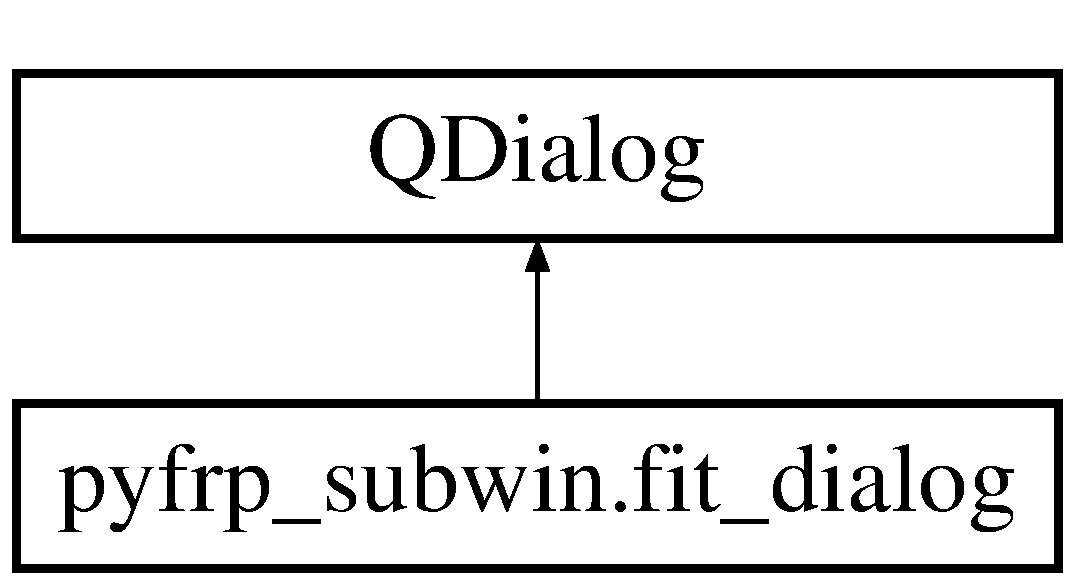
\includegraphics[height=2.000000cm]{classpyfrp__subwin_1_1fit__dialog}
\end{center}
\end{figure}
\subsection*{Public Member Functions}
\begin{DoxyCompactItemize}
\item 
\hypertarget{classpyfrp__subwin_1_1fit__dialog_ac5e6d62900ce2b7f44041ce940fba146}{def {\bfseries \+\_\+\+\_\+init\+\_\+\+\_\+}}\label{classpyfrp__subwin_1_1fit__dialog_ac5e6d62900ce2b7f44041ce940fba146}

\item 
\hypertarget{classpyfrp__subwin_1_1fit__dialog_ab6a39ff42feab85aa4ced0511677d065}{def {\bfseries set\+\_\+name}}\label{classpyfrp__subwin_1_1fit__dialog_ab6a39ff42feab85aa4ced0511677d065}

\item 
\hypertarget{classpyfrp__subwin_1_1fit__dialog_a1f04814bb939fba023614cae0fd54bf7}{def {\bfseries set\+\_\+opt\+\_\+tol}}\label{classpyfrp__subwin_1_1fit__dialog_a1f04814bb939fba023614cae0fd54bf7}

\item 
\hypertarget{classpyfrp__subwin_1_1fit__dialog_afbad85cc556c85f72d5bd38d52be0690}{def {\bfseries set\+\_\+maxfun}}\label{classpyfrp__subwin_1_1fit__dialog_afbad85cc556c85f72d5bd38d52be0690}

\item 
\hypertarget{classpyfrp__subwin_1_1fit__dialog_a8afd18c1d4297d78704ec9c50b330de7}{def {\bfseries set\+\_\+x0\+\_\+\+D}}\label{classpyfrp__subwin_1_1fit__dialog_a8afd18c1d4297d78704ec9c50b330de7}

\item 
\hypertarget{classpyfrp__subwin_1_1fit__dialog_ac6c12a5a39920f733991bbe0931d3854}{def {\bfseries set\+\_\+x0\+\_\+degr}}\label{classpyfrp__subwin_1_1fit__dialog_ac6c12a5a39920f733991bbe0931d3854}

\item 
\hypertarget{classpyfrp__subwin_1_1fit__dialog_ab1c06f3336d1e5c9db34a2f752439229}{def {\bfseries set\+\_\+x0\+\_\+prod}}\label{classpyfrp__subwin_1_1fit__dialog_ab1c06f3336d1e5c9db34a2f752439229}

\item 
\hypertarget{classpyfrp__subwin_1_1fit__dialog_afee30ef0df27f1efa63c9aeb8fe0cf4b}{def {\bfseries set\+\_\+\+U\+B\+\_\+\+D}}\label{classpyfrp__subwin_1_1fit__dialog_afee30ef0df27f1efa63c9aeb8fe0cf4b}

\item 
\hypertarget{classpyfrp__subwin_1_1fit__dialog_aa0350ad1a85c53f293d22fae8c15119a}{def {\bfseries set\+\_\+\+U\+B\+\_\+degr}}\label{classpyfrp__subwin_1_1fit__dialog_aa0350ad1a85c53f293d22fae8c15119a}

\item 
\hypertarget{classpyfrp__subwin_1_1fit__dialog_ab9b28f3cf7c5cbd4eba59d2c68e09038}{def {\bfseries set\+\_\+\+U\+B\+\_\+prod}}\label{classpyfrp__subwin_1_1fit__dialog_ab9b28f3cf7c5cbd4eba59d2c68e09038}

\item 
\hypertarget{classpyfrp__subwin_1_1fit__dialog_a90436f7d207a433cca64ab72b3f23b57}{def {\bfseries set\+\_\+\+L\+B\+\_\+\+D}}\label{classpyfrp__subwin_1_1fit__dialog_a90436f7d207a433cca64ab72b3f23b57}

\item 
\hypertarget{classpyfrp__subwin_1_1fit__dialog_a0f274e63e64839255734714910b471d6}{def {\bfseries set\+\_\+\+L\+B\+\_\+degr}}\label{classpyfrp__subwin_1_1fit__dialog_a0f274e63e64839255734714910b471d6}

\item 
\hypertarget{classpyfrp__subwin_1_1fit__dialog_a0dd5db35b0fc01db8fef20e5ff4a0e5e}{def {\bfseries set\+\_\+\+L\+B\+\_\+prod}}\label{classpyfrp__subwin_1_1fit__dialog_a0dd5db35b0fc01db8fef20e5ff4a0e5e}

\item 
\hypertarget{classpyfrp__subwin_1_1fit__dialog_a631f45d539302e216284e04cb5f8f8ad}{def {\bfseries set\+\_\+cut\+\_\+off\+\_\+t}}\label{classpyfrp__subwin_1_1fit__dialog_a631f45d539302e216284e04cb5f8f8ad}

\item 
\hypertarget{classpyfrp__subwin_1_1fit__dialog_a90bd7118e8ecb9741a6cadbd62ed6ca8}{def {\bfseries sel\+\_\+meth}}\label{classpyfrp__subwin_1_1fit__dialog_a90bd7118e8ecb9741a6cadbd62ed6ca8}

\item 
\hypertarget{classpyfrp__subwin_1_1fit__dialog_ab9f788a643ed1759cf7c1d440bf78bbe}{def {\bfseries update\+\_\+bounds\+\_\+after\+\_\+meth}}\label{classpyfrp__subwin_1_1fit__dialog_ab9f788a643ed1759cf7c1d440bf78bbe}

\item 
\hypertarget{classpyfrp__subwin_1_1fit__dialog_a0def4db03e97a6e3243e3e2e46024522}{def {\bfseries bounds\+\_\+for\+\_\+brute}}\label{classpyfrp__subwin_1_1fit__dialog_a0def4db03e97a6e3243e3e2e46024522}

\item 
\hypertarget{classpyfrp__subwin_1_1fit__dialog_a3e938827af76733e407c9789afa5deb1}{def {\bfseries check\+\_\+equ}}\label{classpyfrp__subwin_1_1fit__dialog_a3e938827af76733e407c9789afa5deb1}

\item 
\hypertarget{classpyfrp__subwin_1_1fit__dialog_a50c4488101781ef93b93044c68bb7b3f}{def {\bfseries check\+\_\+pin}}\label{classpyfrp__subwin_1_1fit__dialog_a50c4488101781ef93b93044c68bb7b3f}

\item 
\hypertarget{classpyfrp__subwin_1_1fit__dialog_ac6c45bc9b271e01d2a90c7a539df92ab}{def {\bfseries check\+\_\+cut}}\label{classpyfrp__subwin_1_1fit__dialog_ac6c45bc9b271e01d2a90c7a539df92ab}

\item 
\hypertarget{classpyfrp__subwin_1_1fit__dialog_a56db90bd4ff3b9e310f9768ea42a81c3}{def {\bfseries check\+\_\+fit\+\_\+out}}\label{classpyfrp__subwin_1_1fit__dialog_a56db90bd4ff3b9e310f9768ea42a81c3}

\item 
\hypertarget{classpyfrp__subwin_1_1fit__dialog_a60b386cd5db5ddd9ce9790b38136e965}{def {\bfseries check\+\_\+fit\+\_\+slice}}\label{classpyfrp__subwin_1_1fit__dialog_a60b386cd5db5ddd9ce9790b38136e965}

\item 
\hypertarget{classpyfrp__subwin_1_1fit__dialog_a2017e4e121e535078829ef1d41604758}{def {\bfseries check\+\_\+fit\+\_\+squ}}\label{classpyfrp__subwin_1_1fit__dialog_a2017e4e121e535078829ef1d41604758}

\item 
\hypertarget{classpyfrp__subwin_1_1fit__dialog_a7aa47a09bd05620917aaba6c7499fe28}{def {\bfseries check\+\_\+fit\+\_\+degr}}\label{classpyfrp__subwin_1_1fit__dialog_a7aa47a09bd05620917aaba6c7499fe28}

\item 
\hypertarget{classpyfrp__subwin_1_1fit__dialog_a921da5e5b88179f097467a21168e3776}{def {\bfseries check\+\_\+fit\+\_\+prod}}\label{classpyfrp__subwin_1_1fit__dialog_a921da5e5b88179f097467a21168e3776}

\item 
\hypertarget{classpyfrp__subwin_1_1fit__dialog_a44af311b10848e9416940ead15cdebf9}{def {\bfseries check\+\_\+debug\+\_\+fit}}\label{classpyfrp__subwin_1_1fit__dialog_a44af311b10848e9416940ead15cdebf9}

\item 
\hypertarget{classpyfrp__subwin_1_1fit__dialog_a9537c6d2033dd6669de1958a1aa79fa9}{def {\bfseries check\+\_\+save\+\_\+track}}\label{classpyfrp__subwin_1_1fit__dialog_a9537c6d2033dd6669de1958a1aa79fa9}

\item 
\hypertarget{classpyfrp__subwin_1_1fit__dialog_a7e0ee9385d2fee95888ea2c6158d9a56}{def {\bfseries check\+\_\+bound\+\_\+\+L\+B\+\_\+\+D}}\label{classpyfrp__subwin_1_1fit__dialog_a7e0ee9385d2fee95888ea2c6158d9a56}

\item 
\hypertarget{classpyfrp__subwin_1_1fit__dialog_aafc88a103a56ea28c62149fb4a6ca570}{def {\bfseries check\+\_\+bound\+\_\+\+U\+B\+\_\+\+D}}\label{classpyfrp__subwin_1_1fit__dialog_aafc88a103a56ea28c62149fb4a6ca570}

\item 
\hypertarget{classpyfrp__subwin_1_1fit__dialog_a93a34a972e01ae65341f6383f817dad6}{def {\bfseries check\+\_\+bound\+\_\+\+L\+B\+\_\+degr}}\label{classpyfrp__subwin_1_1fit__dialog_a93a34a972e01ae65341f6383f817dad6}

\item 
\hypertarget{classpyfrp__subwin_1_1fit__dialog_a8ef89e6ecf495d9d2ee10a587004b90b}{def {\bfseries check\+\_\+bound\+\_\+\+U\+B\+\_\+degr}}\label{classpyfrp__subwin_1_1fit__dialog_a8ef89e6ecf495d9d2ee10a587004b90b}

\item 
\hypertarget{classpyfrp__subwin_1_1fit__dialog_a6639f93991d047c230f2d125e6658771}{def {\bfseries check\+\_\+bound\+\_\+\+L\+B\+\_\+prod}}\label{classpyfrp__subwin_1_1fit__dialog_a6639f93991d047c230f2d125e6658771}

\item 
\hypertarget{classpyfrp__subwin_1_1fit__dialog_a0f0dc32fe811aa90d55990b6759353a3}{def {\bfseries check\+\_\+bound\+\_\+\+U\+B\+\_\+prod}}\label{classpyfrp__subwin_1_1fit__dialog_a0f0dc32fe811aa90d55990b6759353a3}

\item 
\hypertarget{classpyfrp__subwin_1_1fit__dialog_a3dd55d0f007ae4e19f52d651eaf2f07d}{def {\bfseries done\+\_\+pressed}}\label{classpyfrp__subwin_1_1fit__dialog_a3dd55d0f007ae4e19f52d651eaf2f07d}

\end{DoxyCompactItemize}
\subsection*{Public Attributes}
\begin{DoxyCompactItemize}
\item 
\hypertarget{classpyfrp__subwin_1_1fit__dialog_afb2b71d1e0234813e7f77b528343c37f}{{\bfseries fit}}\label{classpyfrp__subwin_1_1fit__dialog_afb2b71d1e0234813e7f77b528343c37f}

\item 
\hypertarget{classpyfrp__subwin_1_1fit__dialog_ab873bc9734e4afb618a50b5cc23dde93}{{\bfseries molecule}}\label{classpyfrp__subwin_1_1fit__dialog_ab873bc9734e4afb618a50b5cc23dde93}

\item 
\hypertarget{classpyfrp__subwin_1_1fit__dialog_ae0520010e2bf87ced637c98cee8fe357}{{\bfseries embryo}}\label{classpyfrp__subwin_1_1fit__dialog_ae0520010e2bf87ced637c98cee8fe357}

\item 
\hypertarget{classpyfrp__subwin_1_1fit__dialog_a44cd44114becd2d8d2bd9e66ffd18b0d}{{\bfseries temp\+\_\+\+L\+B\+\_\+\+D}}\label{classpyfrp__subwin_1_1fit__dialog_a44cd44114becd2d8d2bd9e66ffd18b0d}

\item 
\hypertarget{classpyfrp__subwin_1_1fit__dialog_a781e524d31da759c922125a94d66443d}{{\bfseries temp\+\_\+\+U\+B\+\_\+\+D}}\label{classpyfrp__subwin_1_1fit__dialog_a781e524d31da759c922125a94d66443d}

\item 
\hypertarget{classpyfrp__subwin_1_1fit__dialog_ab5d5530d90fe911a95bf024b274213dd}{{\bfseries temp\+\_\+\+L\+B\+\_\+degr}}\label{classpyfrp__subwin_1_1fit__dialog_ab5d5530d90fe911a95bf024b274213dd}

\item 
\hypertarget{classpyfrp__subwin_1_1fit__dialog_ab617b6af0dd96a2324f548c27c2d12cc}{{\bfseries temp\+\_\+\+U\+B\+\_\+degr}}\label{classpyfrp__subwin_1_1fit__dialog_ab617b6af0dd96a2324f548c27c2d12cc}

\item 
\hypertarget{classpyfrp__subwin_1_1fit__dialog_a72f1861da7847526d689dadf074d3f7d}{{\bfseries temp\+\_\+\+L\+B\+\_\+prod}}\label{classpyfrp__subwin_1_1fit__dialog_a72f1861da7847526d689dadf074d3f7d}

\item 
\hypertarget{classpyfrp__subwin_1_1fit__dialog_aa191003591d20c9287fbfec099c615d5}{{\bfseries temp\+\_\+\+U\+B\+\_\+prod}}\label{classpyfrp__subwin_1_1fit__dialog_aa191003591d20c9287fbfec099c615d5}

\item 
\hypertarget{classpyfrp__subwin_1_1fit__dialog_a24261de2f96ff89fbc0ea4c7d3ca104a}{{\bfseries btn\+\_\+done}}\label{classpyfrp__subwin_1_1fit__dialog_a24261de2f96ff89fbc0ea4c7d3ca104a}

\item 
\hypertarget{classpyfrp__subwin_1_1fit__dialog_a0ca39981b39fc58b1d34d57e6714398a}{{\bfseries lbl\+\_\+opt\+\_\+parms}}\label{classpyfrp__subwin_1_1fit__dialog_a0ca39981b39fc58b1d34d57e6714398a}

\item 
\hypertarget{classpyfrp__subwin_1_1fit__dialog_a8c180595fd800e9d1cdc33595c274a18}{{\bfseries lbl\+\_\+guess}}\label{classpyfrp__subwin_1_1fit__dialog_a8c180595fd800e9d1cdc33595c274a18}

\item 
\hypertarget{classpyfrp__subwin_1_1fit__dialog_a0cc34a1577b249bc5f2b062878931d82}{{\bfseries lbl\+\_\+bounds}}\label{classpyfrp__subwin_1_1fit__dialog_a0cc34a1577b249bc5f2b062878931d82}

\item 
\hypertarget{classpyfrp__subwin_1_1fit__dialog_a8329008c1b0b641f88e334bbaea36f91}{{\bfseries lbl\+\_\+bounded}}\label{classpyfrp__subwin_1_1fit__dialog_a8329008c1b0b641f88e334bbaea36f91}

\item 
\hypertarget{classpyfrp__subwin_1_1fit__dialog_a911c0ce273394d6be4ece614d9201dac}{{\bfseries lbl\+\_\+fitting}}\label{classpyfrp__subwin_1_1fit__dialog_a911c0ce273394d6be4ece614d9201dac}

\item 
\hypertarget{classpyfrp__subwin_1_1fit__dialog_a0a49cb6171277c1b06e4135d119726a0}{{\bfseries lbl\+\_\+name}}\label{classpyfrp__subwin_1_1fit__dialog_a0a49cb6171277c1b06e4135d119726a0}

\item 
\hypertarget{classpyfrp__subwin_1_1fit__dialog_a069857f39176a3ed2f529771ea097d91}{{\bfseries lbl\+\_\+opt\+\_\+meth}}\label{classpyfrp__subwin_1_1fit__dialog_a069857f39176a3ed2f529771ea097d91}

\item 
\hypertarget{classpyfrp__subwin_1_1fit__dialog_aee3df4f0041105eda30cd338436ac520}{{\bfseries lbl\+\_\+opt\+\_\+tol}}\label{classpyfrp__subwin_1_1fit__dialog_aee3df4f0041105eda30cd338436ac520}

\item 
\hypertarget{classpyfrp__subwin_1_1fit__dialog_ace9ed2d764304eb0c45d612eaa81edb5}{{\bfseries lbl\+\_\+maxfun}}\label{classpyfrp__subwin_1_1fit__dialog_ace9ed2d764304eb0c45d612eaa81edb5}

\item 
\hypertarget{classpyfrp__subwin_1_1fit__dialog_a74857afe069b2addba373bad8cf826b2}{{\bfseries lbl\+\_\+save\+\_\+track}}\label{classpyfrp__subwin_1_1fit__dialog_a74857afe069b2addba373bad8cf826b2}

\item 
\hypertarget{classpyfrp__subwin_1_1fit__dialog_aa6ad98168b29b1b0252487b6f940f681}{{\bfseries lbl\+\_\+debug\+\_\+fit}}\label{classpyfrp__subwin_1_1fit__dialog_aa6ad98168b29b1b0252487b6f940f681}

\item 
\hypertarget{classpyfrp__subwin_1_1fit__dialog_aa768c62aacb50c1079e9d99c35d648b8}{{\bfseries lbl\+\_\+x0\+\_\+\+D}}\label{classpyfrp__subwin_1_1fit__dialog_aa768c62aacb50c1079e9d99c35d648b8}

\item 
\hypertarget{classpyfrp__subwin_1_1fit__dialog_a1dd7c8fda1a0eba30e766458efc40b4a}{{\bfseries lbl\+\_\+x0\+\_\+degr}}\label{classpyfrp__subwin_1_1fit__dialog_a1dd7c8fda1a0eba30e766458efc40b4a}

\item 
\hypertarget{classpyfrp__subwin_1_1fit__dialog_acf63aec7e13aa4bbae0a8ba4504b531d}{{\bfseries lbl\+\_\+x0\+\_\+prod}}\label{classpyfrp__subwin_1_1fit__dialog_acf63aec7e13aa4bbae0a8ba4504b531d}

\item 
\hypertarget{classpyfrp__subwin_1_1fit__dialog_ab52f382ab475bc28b79824f9dd220cd1}{{\bfseries lbl\+\_\+\+L\+B\+\_\+\+D}}\label{classpyfrp__subwin_1_1fit__dialog_ab52f382ab475bc28b79824f9dd220cd1}

\item 
\hypertarget{classpyfrp__subwin_1_1fit__dialog_a4013dc4427584d3e2f473948b0f1033e}{{\bfseries lbl\+\_\+\+U\+B\+\_\+\+D}}\label{classpyfrp__subwin_1_1fit__dialog_a4013dc4427584d3e2f473948b0f1033e}

\item 
\hypertarget{classpyfrp__subwin_1_1fit__dialog_a2d1202dc81833a6a97e061890b42e235}{{\bfseries lbl\+\_\+\+L\+B\+\_\+prod}}\label{classpyfrp__subwin_1_1fit__dialog_a2d1202dc81833a6a97e061890b42e235}

\item 
\hypertarget{classpyfrp__subwin_1_1fit__dialog_a0de1d000ffcfb8a7ea20a501e4c94738}{{\bfseries lbl\+\_\+\+U\+B\+\_\+prod}}\label{classpyfrp__subwin_1_1fit__dialog_a0de1d000ffcfb8a7ea20a501e4c94738}

\item 
\hypertarget{classpyfrp__subwin_1_1fit__dialog_a77a88c49df13dafbe2f8e30c74debc5f}{{\bfseries lbl\+\_\+\+L\+B\+\_\+degr}}\label{classpyfrp__subwin_1_1fit__dialog_a77a88c49df13dafbe2f8e30c74debc5f}

\item 
\hypertarget{classpyfrp__subwin_1_1fit__dialog_a902f0d0dd669bcafd21525cbc512796d}{{\bfseries lbl\+\_\+\+U\+B\+\_\+degr}}\label{classpyfrp__subwin_1_1fit__dialog_a902f0d0dd669bcafd21525cbc512796d}

\item 
\hypertarget{classpyfrp__subwin_1_1fit__dialog_a4ef68249ce57489375e295eda308e6ff}{{\bfseries lbl\+\_\+fit\+\_\+out}}\label{classpyfrp__subwin_1_1fit__dialog_a4ef68249ce57489375e295eda308e6ff}

\item 
\hypertarget{classpyfrp__subwin_1_1fit__dialog_a9dc5fc34f7d9c4b5bc129897461a60bf}{{\bfseries lbl\+\_\+fit\+\_\+squ}}\label{classpyfrp__subwin_1_1fit__dialog_a9dc5fc34f7d9c4b5bc129897461a60bf}

\item 
\hypertarget{classpyfrp__subwin_1_1fit__dialog_a5dd99c445cbcf604a186a038a882f96c}{{\bfseries lbl\+\_\+fit\+\_\+slice}}\label{classpyfrp__subwin_1_1fit__dialog_a5dd99c445cbcf604a186a038a882f96c}

\item 
\hypertarget{classpyfrp__subwin_1_1fit__dialog_a862b1cad654a64d30986b6e6afe3086f}{{\bfseries lbl\+\_\+fit\+\_\+prod}}\label{classpyfrp__subwin_1_1fit__dialog_a862b1cad654a64d30986b6e6afe3086f}

\item 
\hypertarget{classpyfrp__subwin_1_1fit__dialog_a03d6152fb3d27c94259ef5de53a982c6}{{\bfseries lbl\+\_\+fit\+\_\+degr}}\label{classpyfrp__subwin_1_1fit__dialog_a03d6152fb3d27c94259ef5de53a982c6}

\item 
\hypertarget{classpyfrp__subwin_1_1fit__dialog_a60584a3ea38846c968ede20fe989c82c}{{\bfseries lbl\+\_\+eq}}\label{classpyfrp__subwin_1_1fit__dialog_a60584a3ea38846c968ede20fe989c82c}

\item 
\hypertarget{classpyfrp__subwin_1_1fit__dialog_ac4ea806b036047a11cfe0437548225c7}{{\bfseries lbl\+\_\+pin}}\label{classpyfrp__subwin_1_1fit__dialog_ac4ea806b036047a11cfe0437548225c7}

\item 
\hypertarget{classpyfrp__subwin_1_1fit__dialog_aa3eab9762efc1c1f134f8377c27a4fa0}{{\bfseries lbl\+\_\+cut\+\_\+off}}\label{classpyfrp__subwin_1_1fit__dialog_aa3eab9762efc1c1f134f8377c27a4fa0}

\item 
\hypertarget{classpyfrp__subwin_1_1fit__dialog_a57ec8e403306c3d71215feb9fa16d1eb}{{\bfseries lbl\+\_\+cut\+\_\+off\+\_\+t}}\label{classpyfrp__subwin_1_1fit__dialog_a57ec8e403306c3d71215feb9fa16d1eb}

\item 
\hypertarget{classpyfrp__subwin_1_1fit__dialog_a46db46ffbe9f88bd02a30a824bda4c75}{{\bfseries combo\+\_\+meth}}\label{classpyfrp__subwin_1_1fit__dialog_a46db46ffbe9f88bd02a30a824bda4c75}

\item 
\hypertarget{classpyfrp__subwin_1_1fit__dialog_a2795264857feb7cbb725b48a494582e9}{{\bfseries qle\+\_\+name}}\label{classpyfrp__subwin_1_1fit__dialog_a2795264857feb7cbb725b48a494582e9}

\item 
\hypertarget{classpyfrp__subwin_1_1fit__dialog_a0d1ec2631145415d1e8212de83d2bc4a}{{\bfseries qle\+\_\+opt\+\_\+tol}}\label{classpyfrp__subwin_1_1fit__dialog_a0d1ec2631145415d1e8212de83d2bc4a}

\item 
\hypertarget{classpyfrp__subwin_1_1fit__dialog_ac507d2c5ad9b0c2861867d77bbc0aced}{{\bfseries qle\+\_\+maxfun}}\label{classpyfrp__subwin_1_1fit__dialog_ac507d2c5ad9b0c2861867d77bbc0aced}

\item 
\hypertarget{classpyfrp__subwin_1_1fit__dialog_a3531fa542bb7cc963a076be76e01db50}{{\bfseries qle\+\_\+x0\+\_\+\+D}}\label{classpyfrp__subwin_1_1fit__dialog_a3531fa542bb7cc963a076be76e01db50}

\item 
\hypertarget{classpyfrp__subwin_1_1fit__dialog_a37af4f36a3b40ba69a11a6379a0b8758}{{\bfseries qle\+\_\+x0\+\_\+degr}}\label{classpyfrp__subwin_1_1fit__dialog_a37af4f36a3b40ba69a11a6379a0b8758}

\item 
\hypertarget{classpyfrp__subwin_1_1fit__dialog_af6bedacc35b8ae8be63fbf8793614741}{{\bfseries qle\+\_\+x0\+\_\+prod}}\label{classpyfrp__subwin_1_1fit__dialog_af6bedacc35b8ae8be63fbf8793614741}

\item 
\hypertarget{classpyfrp__subwin_1_1fit__dialog_a793c7f70e15ce005371acd22638c1ca5}{{\bfseries qle\+\_\+cut\+\_\+off\+\_\+t}}\label{classpyfrp__subwin_1_1fit__dialog_a793c7f70e15ce005371acd22638c1ca5}

\item 
\hypertarget{classpyfrp__subwin_1_1fit__dialog_ab11fdcee6207e26bc85c5b35701440c6}{{\bfseries qle\+\_\+\+L\+B\+\_\+\+D}}\label{classpyfrp__subwin_1_1fit__dialog_ab11fdcee6207e26bc85c5b35701440c6}

\item 
\hypertarget{classpyfrp__subwin_1_1fit__dialog_ac907c237e4c07399b979a55306b9c92d}{{\bfseries qle\+\_\+\+U\+B\+\_\+\+D}}\label{classpyfrp__subwin_1_1fit__dialog_ac907c237e4c07399b979a55306b9c92d}

\item 
\hypertarget{classpyfrp__subwin_1_1fit__dialog_a30a2d2dd5b5693c851539211d86d49bd}{{\bfseries qle\+\_\+\+L\+B\+\_\+degr}}\label{classpyfrp__subwin_1_1fit__dialog_a30a2d2dd5b5693c851539211d86d49bd}

\item 
\hypertarget{classpyfrp__subwin_1_1fit__dialog_a3b9acafeea0a42b0da24aeff1501c086}{{\bfseries qle\+\_\+\+U\+B\+\_\+degr}}\label{classpyfrp__subwin_1_1fit__dialog_a3b9acafeea0a42b0da24aeff1501c086}

\item 
\hypertarget{classpyfrp__subwin_1_1fit__dialog_a9cc5ac2bdf3e47021fcd1d4d4d697cae}{{\bfseries qle\+\_\+\+L\+B\+\_\+prod}}\label{classpyfrp__subwin_1_1fit__dialog_a9cc5ac2bdf3e47021fcd1d4d4d697cae}

\item 
\hypertarget{classpyfrp__subwin_1_1fit__dialog_adc8d08a36f158d876bfcd231bdd2aa7c}{{\bfseries qle\+\_\+\+U\+B\+\_\+prod}}\label{classpyfrp__subwin_1_1fit__dialog_adc8d08a36f158d876bfcd231bdd2aa7c}

\item 
\hypertarget{classpyfrp__subwin_1_1fit__dialog_a15ca56887d0e57266a4973ad7adaa948}{{\bfseries double\+\_\+valid}}\label{classpyfrp__subwin_1_1fit__dialog_a15ca56887d0e57266a4973ad7adaa948}

\item 
\hypertarget{classpyfrp__subwin_1_1fit__dialog_aecbdb6df032777045797046c6eb4946a}{{\bfseries cb\+\_\+debug\+\_\+fit}}\label{classpyfrp__subwin_1_1fit__dialog_aecbdb6df032777045797046c6eb4946a}

\item 
\hypertarget{classpyfrp__subwin_1_1fit__dialog_a5730f7c6a67f42332ff2a07836a9e28f}{{\bfseries cb\+\_\+save\+\_\+track}}\label{classpyfrp__subwin_1_1fit__dialog_a5730f7c6a67f42332ff2a07836a9e28f}

\item 
\hypertarget{classpyfrp__subwin_1_1fit__dialog_ae119530a650e0e610dde71b1f6ec804e}{{\bfseries cb\+\_\+bound\+\_\+\+L\+B\+\_\+\+D}}\label{classpyfrp__subwin_1_1fit__dialog_ae119530a650e0e610dde71b1f6ec804e}

\item 
\hypertarget{classpyfrp__subwin_1_1fit__dialog_af505b6fd30f67289593be8221142407b}{{\bfseries cb\+\_\+bound\+\_\+\+L\+B\+\_\+degr}}\label{classpyfrp__subwin_1_1fit__dialog_af505b6fd30f67289593be8221142407b}

\item 
\hypertarget{classpyfrp__subwin_1_1fit__dialog_a4a0cb2352c95626b9f17e6d595722770}{{\bfseries cb\+\_\+bound\+\_\+\+L\+B\+\_\+prod}}\label{classpyfrp__subwin_1_1fit__dialog_a4a0cb2352c95626b9f17e6d595722770}

\item 
\hypertarget{classpyfrp__subwin_1_1fit__dialog_a60469346c1d8eec1b20e749dab3862a9}{{\bfseries cb\+\_\+bound\+\_\+\+U\+B\+\_\+\+D}}\label{classpyfrp__subwin_1_1fit__dialog_a60469346c1d8eec1b20e749dab3862a9}

\item 
\hypertarget{classpyfrp__subwin_1_1fit__dialog_a8c9e2124079839769e98f33b14742c53}{{\bfseries cb\+\_\+bound\+\_\+\+U\+B\+\_\+degr}}\label{classpyfrp__subwin_1_1fit__dialog_a8c9e2124079839769e98f33b14742c53}

\item 
\hypertarget{classpyfrp__subwin_1_1fit__dialog_a1f3f42b0507c95b64c8e929b23f6fe21}{{\bfseries cb\+\_\+bound\+\_\+\+U\+B\+\_\+prod}}\label{classpyfrp__subwin_1_1fit__dialog_a1f3f42b0507c95b64c8e929b23f6fe21}

\item 
\hypertarget{classpyfrp__subwin_1_1fit__dialog_a8d6de17695c760a42fd1912152820aa8}{{\bfseries cb\+\_\+fit\+\_\+out}}\label{classpyfrp__subwin_1_1fit__dialog_a8d6de17695c760a42fd1912152820aa8}

\item 
\hypertarget{classpyfrp__subwin_1_1fit__dialog_a3d00c6a874ab4652cfa1a2d56dfbba83}{{\bfseries cb\+\_\+fit\+\_\+squ}}\label{classpyfrp__subwin_1_1fit__dialog_a3d00c6a874ab4652cfa1a2d56dfbba83}

\item 
\hypertarget{classpyfrp__subwin_1_1fit__dialog_a7faaba7677d88bb403101e21f56bad4f}{{\bfseries cb\+\_\+fit\+\_\+slice}}\label{classpyfrp__subwin_1_1fit__dialog_a7faaba7677d88bb403101e21f56bad4f}

\item 
\hypertarget{classpyfrp__subwin_1_1fit__dialog_a06b3d8c92bc078aecb93328b067b883e}{{\bfseries cb\+\_\+fit\+\_\+degr}}\label{classpyfrp__subwin_1_1fit__dialog_a06b3d8c92bc078aecb93328b067b883e}

\item 
\hypertarget{classpyfrp__subwin_1_1fit__dialog_a7dd08dbb140a9a3c0915d8e8057310bf}{{\bfseries cb\+\_\+fit\+\_\+prod}}\label{classpyfrp__subwin_1_1fit__dialog_a7dd08dbb140a9a3c0915d8e8057310bf}

\item 
\hypertarget{classpyfrp__subwin_1_1fit__dialog_a2a2a09f9c39434d7c99a21980c94698e}{{\bfseries cb\+\_\+eq}}\label{classpyfrp__subwin_1_1fit__dialog_a2a2a09f9c39434d7c99a21980c94698e}

\item 
\hypertarget{classpyfrp__subwin_1_1fit__dialog_ac900e3e8b95ba5d2f754bfd5eda65bd5}{{\bfseries cb\+\_\+pin}}\label{classpyfrp__subwin_1_1fit__dialog_ac900e3e8b95ba5d2f754bfd5eda65bd5}

\item 
\hypertarget{classpyfrp__subwin_1_1fit__dialog_abe458adcbada5750879ae75a0c8a41a2}{{\bfseries cb\+\_\+cut}}\label{classpyfrp__subwin_1_1fit__dialog_abe458adcbada5750879ae75a0c8a41a2}

\end{DoxyCompactItemize}


The documentation for this class was generated from the following file\+:\begin{DoxyCompactItemize}
\item 
/home/alex\+\_\+loc/\+Documents/\+Research/\+Py\+F\+R\+A\+P/\+Code/pyfrp\+\_\+subwin.\+py\end{DoxyCompactItemize}

\hypertarget{classpyfrp__subwin_1_1fitting__mol__thread}{\section{pyfrp\+\_\+subwin.\+fitting\+\_\+mol\+\_\+thread Class Reference}
\label{classpyfrp__subwin_1_1fitting__mol__thread}\index{pyfrp\+\_\+subwin.\+fitting\+\_\+mol\+\_\+thread@{pyfrp\+\_\+subwin.\+fitting\+\_\+mol\+\_\+thread}}
}
Inheritance diagram for pyfrp\+\_\+subwin.\+fitting\+\_\+mol\+\_\+thread\+:\begin{figure}[H]
\begin{center}
\leavevmode
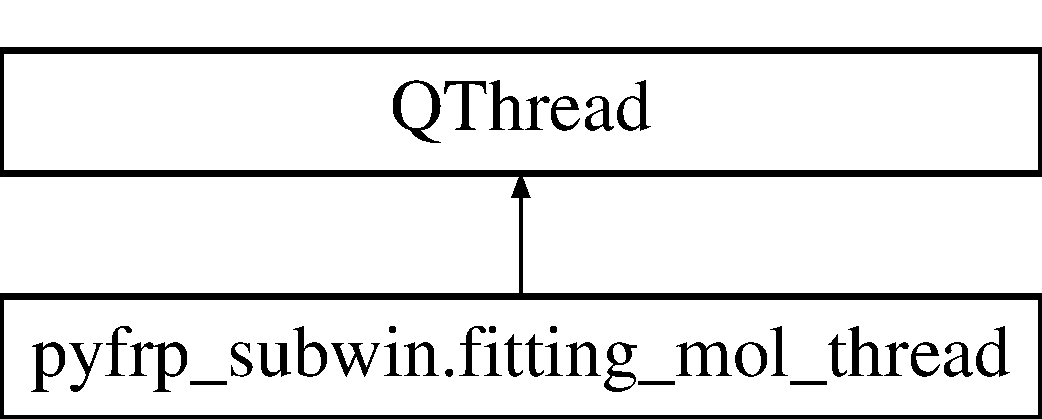
\includegraphics[height=2.000000cm]{classpyfrp__subwin_1_1fitting__mol__thread}
\end{center}
\end{figure}
\subsection*{Public Member Functions}
\begin{DoxyCompactItemize}
\item 
\hypertarget{classpyfrp__subwin_1_1fitting__mol__thread_a12fba29d0487404c420b403d0891e7f2}{def {\bfseries \+\_\+\+\_\+init\+\_\+\+\_\+}}\label{classpyfrp__subwin_1_1fitting__mol__thread_a12fba29d0487404c420b403d0891e7f2}

\item 
\hypertarget{classpyfrp__subwin_1_1fitting__mol__thread_a70ccdacc480cd750b34d1e54eb717f91}{def {\bfseries \+\_\+\+\_\+del\+\_\+\+\_\+}}\label{classpyfrp__subwin_1_1fitting__mol__thread_a70ccdacc480cd750b34d1e54eb717f91}

\item 
\hypertarget{classpyfrp__subwin_1_1fitting__mol__thread_a86a849ef2edbae1a51834603c3a3b2c8}{def {\bfseries run}}\label{classpyfrp__subwin_1_1fitting__mol__thread_a86a849ef2edbae1a51834603c3a3b2c8}

\end{DoxyCompactItemize}
\subsection*{Public Attributes}
\begin{DoxyCompactItemize}
\item 
\hypertarget{classpyfrp__subwin_1_1fitting__mol__thread_abbc0a9d7343ad3510830ef8045a8afe3}{{\bfseries molecule}}\label{classpyfrp__subwin_1_1fitting__mol__thread_abbc0a9d7343ad3510830ef8045a8afe3}

\item 
\hypertarget{classpyfrp__subwin_1_1fitting__mol__thread_a9980778539d2aa614d5140fc1c724944}{{\bfseries gui}}\label{classpyfrp__subwin_1_1fitting__mol__thread_a9980778539d2aa614d5140fc1c724944}

\end{DoxyCompactItemize}
\subsection*{Static Public Attributes}
\begin{DoxyCompactItemize}
\item 
\hypertarget{classpyfrp__subwin_1_1fitting__mol__thread_ad4e8634e61f98eaf8e40f63da9053155}{tuple {\bfseries task\+Finished} = Qt\+Core.\+pyqt\+Signal()}\label{classpyfrp__subwin_1_1fitting__mol__thread_ad4e8634e61f98eaf8e40f63da9053155}

\end{DoxyCompactItemize}


The documentation for this class was generated from the following file\+:\begin{DoxyCompactItemize}
\item 
/home/alex\+\_\+loc/\+Documents/\+Research/\+Py\+F\+R\+A\+P/\+Code/pyfrp\+\_\+subwin.\+py\end{DoxyCompactItemize}

\hypertarget{classpyfrp__subwin_1_1fitting__prog}{\section{pyfrp\+\_\+subwin.\+fitting\+\_\+prog Class Reference}
\label{classpyfrp__subwin_1_1fitting__prog}\index{pyfrp\+\_\+subwin.\+fitting\+\_\+prog@{pyfrp\+\_\+subwin.\+fitting\+\_\+prog}}
}
Inheritance diagram for pyfrp\+\_\+subwin.\+fitting\+\_\+prog\+:\begin{figure}[H]
\begin{center}
\leavevmode
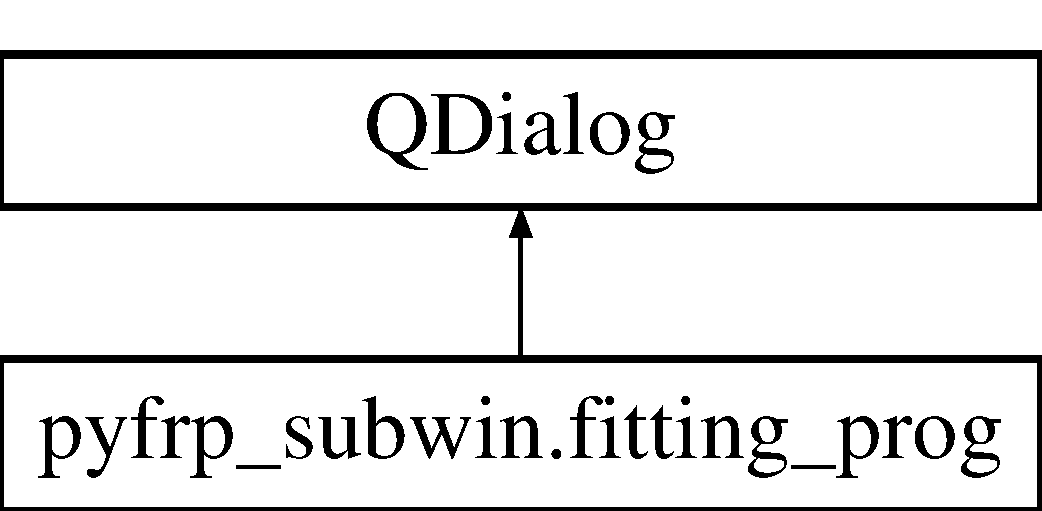
\includegraphics[height=2.000000cm]{classpyfrp__subwin_1_1fitting__prog}
\end{center}
\end{figure}
\subsection*{Public Member Functions}
\begin{DoxyCompactItemize}
\item 
\hypertarget{classpyfrp__subwin_1_1fitting__prog_a14db48e215f6b32d258dda95cb55c0ce}{def {\bfseries \+\_\+\+\_\+init\+\_\+\+\_\+}}\label{classpyfrp__subwin_1_1fitting__prog_a14db48e215f6b32d258dda95cb55c0ce}

\item 
\hypertarget{classpyfrp__subwin_1_1fitting__prog_ac2b67fc4dec25d9f1acbaa6fe995a615}{def {\bfseries cancel\+\_\+fitting}}\label{classpyfrp__subwin_1_1fitting__prog_ac2b67fc4dec25d9f1acbaa6fe995a615}

\end{DoxyCompactItemize}
\subsection*{Public Attributes}
\begin{DoxyCompactItemize}
\item 
\hypertarget{classpyfrp__subwin_1_1fitting__prog_a5108e8d8cfec0951c71267903895f85e}{{\bfseries lbl\+\_\+name}}\label{classpyfrp__subwin_1_1fitting__prog_a5108e8d8cfec0951c71267903895f85e}

\item 
\hypertarget{classpyfrp__subwin_1_1fitting__prog_a09b0b70b71286e0743cfd17338299c8a}{{\bfseries btn\+\_\+cancel}}\label{classpyfrp__subwin_1_1fitting__prog_a09b0b70b71286e0743cfd17338299c8a}

\item 
\hypertarget{classpyfrp__subwin_1_1fitting__prog_a7ede5c97fd9ab41eb756e3d869fabdef}{{\bfseries vbox}}\label{classpyfrp__subwin_1_1fitting__prog_a7ede5c97fd9ab41eb756e3d869fabdef}

\end{DoxyCompactItemize}


The documentation for this class was generated from the following file\+:\begin{DoxyCompactItemize}
\item 
/home/alex\+\_\+loc/\+Documents/\+Research/\+Py\+F\+R\+A\+P/\+Code/pyfrp\+\_\+subwin.\+py\end{DoxyCompactItemize}

\hypertarget{classpyfrp__subwin_1_1fitting__thread}{\section{pyfrp\+\_\+subwin.\+fitting\+\_\+thread Class Reference}
\label{classpyfrp__subwin_1_1fitting__thread}\index{pyfrp\+\_\+subwin.\+fitting\+\_\+thread@{pyfrp\+\_\+subwin.\+fitting\+\_\+thread}}
}
Inheritance diagram for pyfrp\+\_\+subwin.\+fitting\+\_\+thread\+:\begin{figure}[H]
\begin{center}
\leavevmode
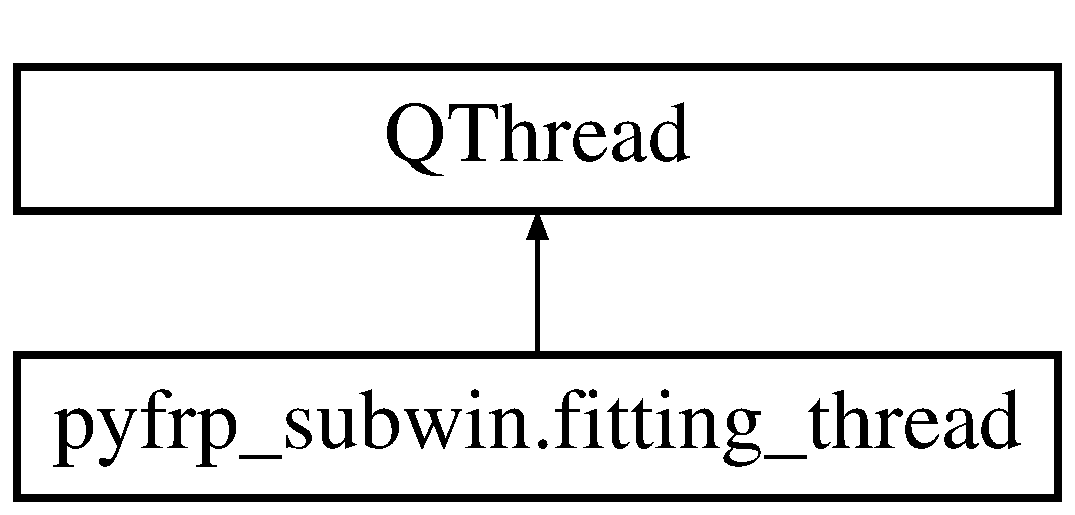
\includegraphics[height=2.000000cm]{classpyfrp__subwin_1_1fitting__thread}
\end{center}
\end{figure}
\subsection*{Public Member Functions}
\begin{DoxyCompactItemize}
\item 
\hypertarget{classpyfrp__subwin_1_1fitting__thread_a135c920b529d2edae9008c8c18d6395a}{def {\bfseries \+\_\+\+\_\+init\+\_\+\+\_\+}}\label{classpyfrp__subwin_1_1fitting__thread_a135c920b529d2edae9008c8c18d6395a}

\item 
\hypertarget{classpyfrp__subwin_1_1fitting__thread_a8c972c271919a9cbe47f8fe04951218f}{def {\bfseries \+\_\+\+\_\+del\+\_\+\+\_\+}}\label{classpyfrp__subwin_1_1fitting__thread_a8c972c271919a9cbe47f8fe04951218f}

\item 
\hypertarget{classpyfrp__subwin_1_1fitting__thread_a0a0c89e456cafdba6deade43af541a19}{def {\bfseries run}}\label{classpyfrp__subwin_1_1fitting__thread_a0a0c89e456cafdba6deade43af541a19}

\end{DoxyCompactItemize}
\subsection*{Public Attributes}
\begin{DoxyCompactItemize}
\item 
\hypertarget{classpyfrp__subwin_1_1fitting__thread_a55703cecdb5dac7573ce1d8928c820a5}{{\bfseries embryo}}\label{classpyfrp__subwin_1_1fitting__thread_a55703cecdb5dac7573ce1d8928c820a5}

\item 
\hypertarget{classpyfrp__subwin_1_1fitting__thread_a1fb3c160a8becf8171df6ebe663f95bc}{{\bfseries fit}}\label{classpyfrp__subwin_1_1fitting__thread_a1fb3c160a8becf8171df6ebe663f95bc}

\item 
\hypertarget{classpyfrp__subwin_1_1fitting__thread_a750ec7f2cd641743b8a957f0334c9b25}{{\bfseries gui}}\label{classpyfrp__subwin_1_1fitting__thread_a750ec7f2cd641743b8a957f0334c9b25}

\end{DoxyCompactItemize}
\subsection*{Static Public Attributes}
\begin{DoxyCompactItemize}
\item 
\hypertarget{classpyfrp__subwin_1_1fitting__thread_a2ef4b0d66377347362787b6c054c8194}{tuple {\bfseries task\+Finished} = Qt\+Core.\+pyqt\+Signal()}\label{classpyfrp__subwin_1_1fitting__thread_a2ef4b0d66377347362787b6c054c8194}

\end{DoxyCompactItemize}


The documentation for this class was generated from the following file\+:\begin{DoxyCompactItemize}
\item 
/home/alex\+\_\+loc/\+Documents/\+Research/\+Py\+F\+R\+A\+P/\+Code/pyfrp\+\_\+subwin.\+py\end{DoxyCompactItemize}

\hypertarget{classpyfrp__subwin_1_1geometry__dialog}{\section{pyfrp\+\_\+subwin.\+geometry\+\_\+dialog Class Reference}
\label{classpyfrp__subwin_1_1geometry__dialog}\index{pyfrp\+\_\+subwin.\+geometry\+\_\+dialog@{pyfrp\+\_\+subwin.\+geometry\+\_\+dialog}}
}
Inheritance diagram for pyfrp\+\_\+subwin.\+geometry\+\_\+dialog\+:\begin{figure}[H]
\begin{center}
\leavevmode
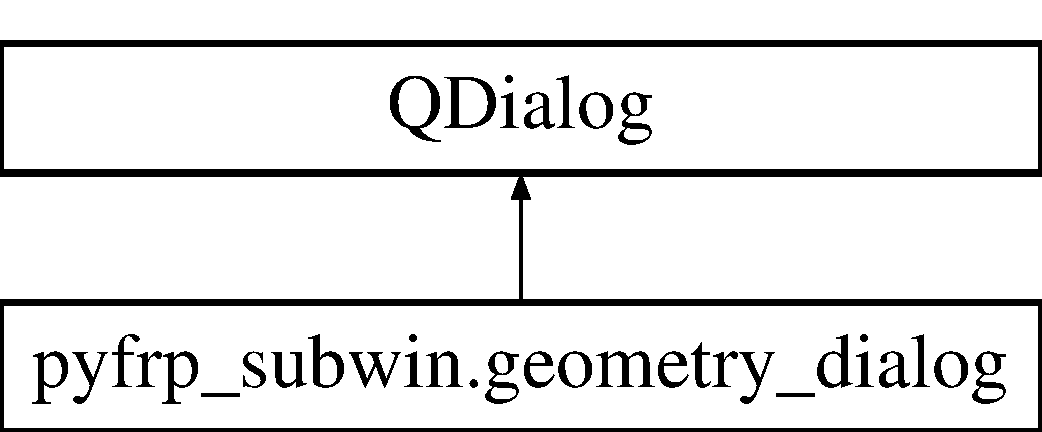
\includegraphics[height=2.000000cm]{classpyfrp__subwin_1_1geometry__dialog}
\end{center}
\end{figure}
\subsection*{Public Member Functions}
\begin{DoxyCompactItemize}
\item 
\hypertarget{classpyfrp__subwin_1_1geometry__dialog_a8d39e5a018a156eb1c1b6e3bfdfa5295}{def {\bfseries \+\_\+\+\_\+init\+\_\+\+\_\+}}\label{classpyfrp__subwin_1_1geometry__dialog_a8d39e5a018a156eb1c1b6e3bfdfa5295}

\item 
\hypertarget{classpyfrp__subwin_1_1geometry__dialog_a41cfb95e4241f7089dda03d9921329a9}{def {\bfseries create\+\_\+frame}}\label{classpyfrp__subwin_1_1geometry__dialog_a41cfb95e4241f7089dda03d9921329a9}

\item 
\hypertarget{classpyfrp__subwin_1_1geometry__dialog_a7d8fc02027fd8a693b1b96ee85cd4e53}{def {\bfseries create\+\_\+canvas}}\label{classpyfrp__subwin_1_1geometry__dialog_a7d8fc02027fd8a693b1b96ee85cd4e53}

\item 
\hypertarget{classpyfrp__subwin_1_1geometry__dialog_a25b8f2ca40a58fabf33653dd5ed667d5}{def {\bfseries sel\+\_\+geom}}\label{classpyfrp__subwin_1_1geometry__dialog_a25b8f2ca40a58fabf33653dd5ed667d5}

\item 
\hypertarget{classpyfrp__subwin_1_1geometry__dialog_a4313586cc51acb23523ca2a7493d5797}{def {\bfseries check\+\_\+img\+\_\+in\+\_\+domain}}\label{classpyfrp__subwin_1_1geometry__dialog_a4313586cc51acb23523ca2a7493d5797}

\item 
\hypertarget{classpyfrp__subwin_1_1geometry__dialog_a512d9462da92bae0f5b6246576ca5a5d}{def {\bfseries set\+\_\+sliceheight}}\label{classpyfrp__subwin_1_1geometry__dialog_a512d9462da92bae0f5b6246576ca5a5d}

\item 
\hypertarget{classpyfrp__subwin_1_1geometry__dialog_ab6a42708c12a1a1e21a1dab0e9c8616f}{def {\bfseries set\+\_\+fish\+\_\+outer\+\_\+radius}}\label{classpyfrp__subwin_1_1geometry__dialog_ab6a42708c12a1a1e21a1dab0e9c8616f}

\item 
\hypertarget{classpyfrp__subwin_1_1geometry__dialog_a4d9c6b61be206625502619e129c61362}{def {\bfseries set\+\_\+frog\+\_\+radius}}\label{classpyfrp__subwin_1_1geometry__dialog_a4d9c6b61be206625502619e129c61362}

\item 
\hypertarget{classpyfrp__subwin_1_1geometry__dialog_a50a7608cbbfe5ae67bd94360e7ba25b4}{def {\bfseries set\+\_\+cyl\+\_\+radius}}\label{classpyfrp__subwin_1_1geometry__dialog_a50a7608cbbfe5ae67bd94360e7ba25b4}

\item 
\hypertarget{classpyfrp__subwin_1_1geometry__dialog_ab23691d4100962512e9d67bbc41e478a}{def {\bfseries set\+\_\+cyl\+\_\+height}}\label{classpyfrp__subwin_1_1geometry__dialog_ab23691d4100962512e9d67bbc41e478a}

\item 
\hypertarget{classpyfrp__subwin_1_1geometry__dialog_a70036087a7495abce9775d6aaf913891}{def {\bfseries build\+\_\+fish}}\label{classpyfrp__subwin_1_1geometry__dialog_a70036087a7495abce9775d6aaf913891}

\item 
\hypertarget{classpyfrp__subwin_1_1geometry__dialog_a953a9fb1652a6fbc7cb993b78f863b8e}{def {\bfseries build\+\_\+frog}}\label{classpyfrp__subwin_1_1geometry__dialog_a953a9fb1652a6fbc7cb993b78f863b8e}

\item 
\hypertarget{classpyfrp__subwin_1_1geometry__dialog_aa6a23c71a81ba2a7f1a5d4ee99c41cae}{def {\bfseries build\+\_\+cylinder}}\label{classpyfrp__subwin_1_1geometry__dialog_aa6a23c71a81ba2a7f1a5d4ee99c41cae}

\item 
\hypertarget{classpyfrp__subwin_1_1geometry__dialog_ab27356244e9e1b378dbc9fb7ca402629}{def {\bfseries plot\+\_\+fish}}\label{classpyfrp__subwin_1_1geometry__dialog_ab27356244e9e1b378dbc9fb7ca402629}

\item 
\hypertarget{classpyfrp__subwin_1_1geometry__dialog_a5249856f0dc56a9df645cf38d97fa4b1}{def {\bfseries plot\+\_\+frog}}\label{classpyfrp__subwin_1_1geometry__dialog_a5249856f0dc56a9df645cf38d97fa4b1}

\item 
\hypertarget{classpyfrp__subwin_1_1geometry__dialog_ae49383aa6318216ee451814efd32e4d2}{def {\bfseries plot\+\_\+cylinder}}\label{classpyfrp__subwin_1_1geometry__dialog_ae49383aa6318216ee451814efd32e4d2}

\item 
\hypertarget{classpyfrp__subwin_1_1geometry__dialog_ab253585e1a4b2ec6f66585621251664a}{def {\bfseries adjust\+\_\+zaxis}}\label{classpyfrp__subwin_1_1geometry__dialog_ab253585e1a4b2ec6f66585621251664a}

\item 
\hypertarget{classpyfrp__subwin_1_1geometry__dialog_a1eeb9d33a17460ef17ed67b2cd987783}{def {\bfseries show\+\_\+img}}\label{classpyfrp__subwin_1_1geometry__dialog_a1eeb9d33a17460ef17ed67b2cd987783}

\item 
\hypertarget{classpyfrp__subwin_1_1geometry__dialog_a60948d34bebb06dcfa49029c456f8e71}{def {\bfseries done\+\_\+pressed}}\label{classpyfrp__subwin_1_1geometry__dialog_a60948d34bebb06dcfa49029c456f8e71}

\end{DoxyCompactItemize}
\subsection*{Public Attributes}
\begin{DoxyCompactItemize}
\item 
\hypertarget{classpyfrp__subwin_1_1geometry__dialog_a601fc382262ce532b0a92e8a41cb988e}{{\bfseries embryo}}\label{classpyfrp__subwin_1_1geometry__dialog_a601fc382262ce532b0a92e8a41cb988e}

\item 
\hypertarget{classpyfrp__subwin_1_1geometry__dialog_a8646f2c13e1b8a39a8ff2fb1f44b1947}{{\bfseries dpi}}\label{classpyfrp__subwin_1_1geometry__dialog_a8646f2c13e1b8a39a8ff2fb1f44b1947}

\item 
\hypertarget{classpyfrp__subwin_1_1geometry__dialog_af9e78087199daedc80c3a1e6c47217e3}{{\bfseries btn\+\_\+done}}\label{classpyfrp__subwin_1_1geometry__dialog_af9e78087199daedc80c3a1e6c47217e3}

\item 
\hypertarget{classpyfrp__subwin_1_1geometry__dialog_aa6f04bb78fe02b4a2174fc0e8ee90842}{{\bfseries lbl\+\_\+geometry}}\label{classpyfrp__subwin_1_1geometry__dialog_aa6f04bb78fe02b4a2174fc0e8ee90842}

\item 
\hypertarget{classpyfrp__subwin_1_1geometry__dialog_a9fd95eaef1472f83c8bd868c546a168d}{{\bfseries lbl\+\_\+img\+\_\+in\+\_\+domain}}\label{classpyfrp__subwin_1_1geometry__dialog_a9fd95eaef1472f83c8bd868c546a168d}

\item 
\hypertarget{classpyfrp__subwin_1_1geometry__dialog_a6a5949ada04874bbbeee589fea253de2}{{\bfseries lbl\+\_\+fish\+\_\+inner\+\_\+radius}}\label{classpyfrp__subwin_1_1geometry__dialog_a6a5949ada04874bbbeee589fea253de2}

\item 
\hypertarget{classpyfrp__subwin_1_1geometry__dialog_a666d5e3778cb0312b77b12656dcf86f8}{{\bfseries lbl\+\_\+fish\+\_\+outer\+\_\+radius}}\label{classpyfrp__subwin_1_1geometry__dialog_a666d5e3778cb0312b77b12656dcf86f8}

\item 
\hypertarget{classpyfrp__subwin_1_1geometry__dialog_a84645fa53aaf91c2b7fdad8c968e652f}{{\bfseries lbl\+\_\+fish\+\_\+dist}}\label{classpyfrp__subwin_1_1geometry__dialog_a84645fa53aaf91c2b7fdad8c968e652f}

\item 
\hypertarget{classpyfrp__subwin_1_1geometry__dialog_acc6263111050ffd60a4c9d2fca23dd66}{{\bfseries lbl\+\_\+cyl\+\_\+radius}}\label{classpyfrp__subwin_1_1geometry__dialog_acc6263111050ffd60a4c9d2fca23dd66}

\item 
\hypertarget{classpyfrp__subwin_1_1geometry__dialog_af43ddedde71cde7a0836259b221b0d97}{{\bfseries lbl\+\_\+cyl\+\_\+height}}\label{classpyfrp__subwin_1_1geometry__dialog_af43ddedde71cde7a0836259b221b0d97}

\item 
\hypertarget{classpyfrp__subwin_1_1geometry__dialog_af3039e75b8bf8b44af27689b71cbe3f5}{{\bfseries lbl\+\_\+frog\+\_\+radius}}\label{classpyfrp__subwin_1_1geometry__dialog_af3039e75b8bf8b44af27689b71cbe3f5}

\item 
\hypertarget{classpyfrp__subwin_1_1geometry__dialog_ac2a6dbf9a317fef61df93c46e86d0a1c}{{\bfseries lbl\+\_\+slice\+\_\+height}}\label{classpyfrp__subwin_1_1geometry__dialog_ac2a6dbf9a317fef61df93c46e86d0a1c}

\item 
\hypertarget{classpyfrp__subwin_1_1geometry__dialog_a0385575a9a6871dfa1783c8650bcc1ba}{{\bfseries combo\+\_\+geom}}\label{classpyfrp__subwin_1_1geometry__dialog_a0385575a9a6871dfa1783c8650bcc1ba}

\item 
\hypertarget{classpyfrp__subwin_1_1geometry__dialog_a70de5a02891e01ac43a0700847bcb46c}{{\bfseries qle\+\_\+slice\+\_\+height}}\label{classpyfrp__subwin_1_1geometry__dialog_a70de5a02891e01ac43a0700847bcb46c}

\item 
\hypertarget{classpyfrp__subwin_1_1geometry__dialog_a5243b0c4335833c2d756e1733e4c1746}{{\bfseries qle\+\_\+fish\+\_\+inner\+\_\+radius}}\label{classpyfrp__subwin_1_1geometry__dialog_a5243b0c4335833c2d756e1733e4c1746}

\item 
\hypertarget{classpyfrp__subwin_1_1geometry__dialog_a923d12c5cd2212aa40693e5848de702c}{{\bfseries qle\+\_\+fish\+\_\+outer\+\_\+radius}}\label{classpyfrp__subwin_1_1geometry__dialog_a923d12c5cd2212aa40693e5848de702c}

\item 
\hypertarget{classpyfrp__subwin_1_1geometry__dialog_a08b14ab017dec034dcf3d26786c72206}{{\bfseries qle\+\_\+fish\+\_\+dist}}\label{classpyfrp__subwin_1_1geometry__dialog_a08b14ab017dec034dcf3d26786c72206}

\item 
\hypertarget{classpyfrp__subwin_1_1geometry__dialog_aff03f4c77f3e33cc2df11066c7b235df}{{\bfseries qle\+\_\+frog\+\_\+radius}}\label{classpyfrp__subwin_1_1geometry__dialog_aff03f4c77f3e33cc2df11066c7b235df}

\item 
\hypertarget{classpyfrp__subwin_1_1geometry__dialog_a59d816e92d535cb3d11e9fcb36f465df}{{\bfseries qle\+\_\+cyl\+\_\+radius}}\label{classpyfrp__subwin_1_1geometry__dialog_a59d816e92d535cb3d11e9fcb36f465df}

\item 
\hypertarget{classpyfrp__subwin_1_1geometry__dialog_a04225149332ba7992c692ca2681b9b0b}{{\bfseries qle\+\_\+cyl\+\_\+height}}\label{classpyfrp__subwin_1_1geometry__dialog_a04225149332ba7992c692ca2681b9b0b}

\item 
\hypertarget{classpyfrp__subwin_1_1geometry__dialog_af85bcb5269e371fd2075979d45a48f2d}{{\bfseries double\+\_\+valid}}\label{classpyfrp__subwin_1_1geometry__dialog_af85bcb5269e371fd2075979d45a48f2d}

\item 
\hypertarget{classpyfrp__subwin_1_1geometry__dialog_aa48db198848beeb0ab1ce863a84239ef}{{\bfseries cb\+\_\+img\+\_\+in\+\_\+domain}}\label{classpyfrp__subwin_1_1geometry__dialog_aa48db198848beeb0ab1ce863a84239ef}

\item 
\hypertarget{classpyfrp__subwin_1_1geometry__dialog_a0bbf6e041a275349cec04daca93ede15}{{\bfseries plot\+\_\+frame}}\label{classpyfrp__subwin_1_1geometry__dialog_a0bbf6e041a275349cec04daca93ede15}

\item 
\hypertarget{classpyfrp__subwin_1_1geometry__dialog_a2690e455c16124c0acacd7ca6e61f7fe}{{\bfseries vbox}}\label{classpyfrp__subwin_1_1geometry__dialog_a2690e455c16124c0acacd7ca6e61f7fe}

\item 
\hypertarget{classpyfrp__subwin_1_1geometry__dialog_a1e06d8e8be3608ac316c199ed7d90149}{{\bfseries hbox}}\label{classpyfrp__subwin_1_1geometry__dialog_a1e06d8e8be3608ac316c199ed7d90149}

\item 
\hypertarget{classpyfrp__subwin_1_1geometry__dialog_ab30dcaf8de9734ac78ef7ea4d23b5ae2}{{\bfseries fig}}\label{classpyfrp__subwin_1_1geometry__dialog_ab30dcaf8de9734ac78ef7ea4d23b5ae2}

\item 
\hypertarget{classpyfrp__subwin_1_1geometry__dialog_a16bc9aebebcf848672ef9d78ebeace64}{{\bfseries canvas}}\label{classpyfrp__subwin_1_1geometry__dialog_a16bc9aebebcf848672ef9d78ebeace64}

\item 
\hypertarget{classpyfrp__subwin_1_1geometry__dialog_ad3856b746dc6129ab1bc2da530b8b1ae}{{\bfseries ax}}\label{classpyfrp__subwin_1_1geometry__dialog_ad3856b746dc6129ab1bc2da530b8b1ae}

\item 
\hypertarget{classpyfrp__subwin_1_1geometry__dialog_a14d66928e5a3356137f8c2e7aaef363c}{{\bfseries file\+\_\+list}}\label{classpyfrp__subwin_1_1geometry__dialog_a14d66928e5a3356137f8c2e7aaef363c}

\end{DoxyCompactItemize}


The documentation for this class was generated from the following file\+:\begin{DoxyCompactItemize}
\item 
/home/alex\+\_\+loc/\+Documents/\+Research/\+Py\+F\+R\+A\+P/\+Code/pyfrp\+\_\+subwin.\+py\end{DoxyCompactItemize}

\hypertarget{classpyfrp__term_1_1PyInterp_1_1InteractiveInterpreter}{\section{pyfrp\+\_\+term.\+Py\+Interp.\+Interactive\+Interpreter Class Reference}
\label{classpyfrp__term_1_1PyInterp_1_1InteractiveInterpreter}\index{pyfrp\+\_\+term.\+Py\+Interp.\+Interactive\+Interpreter@{pyfrp\+\_\+term.\+Py\+Interp.\+Interactive\+Interpreter}}
}
Inheritance diagram for pyfrp\+\_\+term.\+Py\+Interp.\+Interactive\+Interpreter\+:\begin{figure}[H]
\begin{center}
\leavevmode
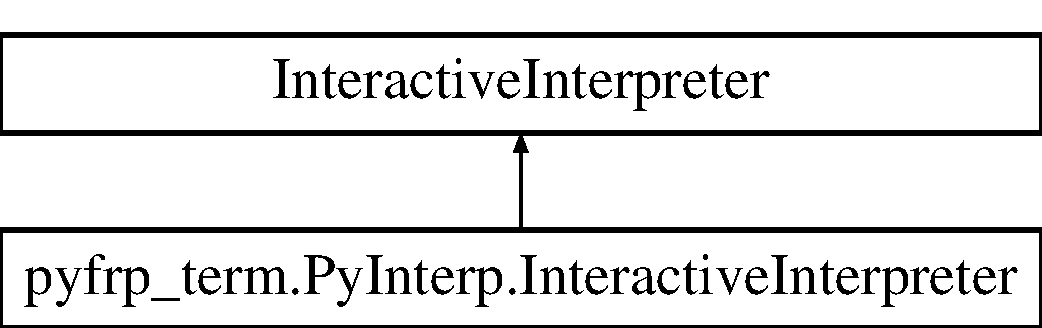
\includegraphics[height=2.000000cm]{classpyfrp__term_1_1PyInterp_1_1InteractiveInterpreter}
\end{center}
\end{figure}
\subsection*{Public Member Functions}
\begin{DoxyCompactItemize}
\item 
\hypertarget{classpyfrp__term_1_1PyInterp_1_1InteractiveInterpreter_a5f8b5d51f33e379f60151591a3761d54}{def {\bfseries \+\_\+\+\_\+init\+\_\+\+\_\+}}\label{classpyfrp__term_1_1PyInterp_1_1InteractiveInterpreter_a5f8b5d51f33e379f60151591a3761d54}

\item 
\hypertarget{classpyfrp__term_1_1PyInterp_1_1InteractiveInterpreter_a4eea442886b0170d3baf23ae9634b425}{def {\bfseries run\+It}}\label{classpyfrp__term_1_1PyInterp_1_1InteractiveInterpreter_a4eea442886b0170d3baf23ae9634b425}

\end{DoxyCompactItemize}


The documentation for this class was generated from the following file\+:\begin{DoxyCompactItemize}
\item 
/home/alex\+\_\+loc/\+Documents/\+Research/\+Py\+F\+R\+A\+P/\+Code/pyfrp\+\_\+term.\+py\end{DoxyCompactItemize}

\hypertarget{classmolecule_1_1molecule}{\section{molecule.\+molecule Class Reference}
\label{classmolecule_1_1molecule}\index{molecule.\+molecule@{molecule.\+molecule}}
}
\subsection*{Public Member Functions}
\begin{DoxyCompactItemize}
\item 
\hypertarget{classmolecule_1_1molecule_a6ab0eb481e397971fd9be5fae8254058}{def {\bfseries \+\_\+\+\_\+init\+\_\+\+\_\+}}\label{classmolecule_1_1molecule_a6ab0eb481e397971fd9be5fae8254058}

\item 
\hypertarget{classmolecule_1_1molecule_a13d8cf866d50513a01855f15327752a4}{def {\bfseries add\+\_\+embryo}}\label{classmolecule_1_1molecule_a13d8cf866d50513a01855f15327752a4}

\item 
\hypertarget{classmolecule_1_1molecule_aa0161c35032bb46571e050ee8b1c7c0e}{def {\bfseries remove\+\_\+embryo}}\label{classmolecule_1_1molecule_aa0161c35032bb46571e050ee8b1c7c0e}

\item 
\hypertarget{classmolecule_1_1molecule_abc1b60549fbfe35caa70a8178d1fb337}{def {\bfseries save\+\_\+molecule}}\label{classmolecule_1_1molecule_abc1b60549fbfe35caa70a8178d1fb337}

\item 
\hypertarget{classmolecule_1_1molecule_a134fa06ba99aa732bc3b6fafcedbe824}{def {\bfseries load\+\_\+molecule}}\label{classmolecule_1_1molecule_a134fa06ba99aa732bc3b6fafcedbe824}

\item 
\hypertarget{classmolecule_1_1molecule_a0f08deb008dfcb9bfaa9b999bced444b}{def {\bfseries sumup\+\_\+results}}\label{classmolecule_1_1molecule_a0f08deb008dfcb9bfaa9b999bced444b}

\end{DoxyCompactItemize}
\subsection*{Public Attributes}
\begin{DoxyCompactItemize}
\item 
\hypertarget{classmolecule_1_1molecule_abae84c526cb895e006f129f203a08fe4}{{\bfseries name}}\label{classmolecule_1_1molecule_abae84c526cb895e006f129f203a08fe4}

\item 
\hypertarget{classmolecule_1_1molecule_abcc7a0506534a79f0f035224a0bbc177}{{\bfseries embryos}}\label{classmolecule_1_1molecule_abcc7a0506534a79f0f035224a0bbc177}

\item 
\hypertarget{classmolecule_1_1molecule_a642853a852dc8fbba5d10dd27df562f0}{{\bfseries sel\+\_\+fits}}\label{classmolecule_1_1molecule_a642853a852dc8fbba5d10dd27df562f0}

\item 
\hypertarget{classmolecule_1_1molecule_a68d7f84c79da4b9c5aacee15df11ba80}{{\bfseries D\+\_\+mu\+\_\+av}}\label{classmolecule_1_1molecule_a68d7f84c79da4b9c5aacee15df11ba80}

\item 
\hypertarget{classmolecule_1_1molecule_a35918be03f4020d910cca2021feb8d69}{{\bfseries prod\+\_\+av}}\label{classmolecule_1_1molecule_a35918be03f4020d910cca2021feb8d69}

\item 
\hypertarget{classmolecule_1_1molecule_a14a48a8abfaacba22113124b128dd704}{{\bfseries degr\+\_\+av}}\label{classmolecule_1_1molecule_a14a48a8abfaacba22113124b128dd704}

\item 
\hypertarget{classmolecule_1_1molecule_a41b2ce201c05986b838d5cbf0e908873}{{\bfseries Rsq\+\_\+av}}\label{classmolecule_1_1molecule_a41b2ce201c05986b838d5cbf0e908873}

\item 
\hypertarget{classmolecule_1_1molecule_ad9ecd9f2005f1704398108c76ba4b4d9}{{\bfseries ssd\+\_\+av}}\label{classmolecule_1_1molecule_ad9ecd9f2005f1704398108c76ba4b4d9}

\item 
\hypertarget{classmolecule_1_1molecule_a96aed906cac15dc395a5f3d26da27bd0}{{\bfseries D\+\_\+mu\+\_\+std}}\label{classmolecule_1_1molecule_a96aed906cac15dc395a5f3d26da27bd0}

\item 
\hypertarget{classmolecule_1_1molecule_af8ec5dec724f3b499b5e5a812bc386b7}{{\bfseries prod\+\_\+std}}\label{classmolecule_1_1molecule_af8ec5dec724f3b499b5e5a812bc386b7}

\item 
\hypertarget{classmolecule_1_1molecule_a30e29c7fb8df751bc99c80e7c8ada6e7}{{\bfseries degr\+\_\+std}}\label{classmolecule_1_1molecule_a30e29c7fb8df751bc99c80e7c8ada6e7}

\item 
\hypertarget{classmolecule_1_1molecule_a65f7b467fe3b18b0910f2f076efb696c}{{\bfseries D\+\_\+mu\+\_\+sterr}}\label{classmolecule_1_1molecule_a65f7b467fe3b18b0910f2f076efb696c}

\item 
\hypertarget{classmolecule_1_1molecule_a5c57b0758221f5020c55b528112e0907}{{\bfseries prod\+\_\+sterr}}\label{classmolecule_1_1molecule_a5c57b0758221f5020c55b528112e0907}

\item 
\hypertarget{classmolecule_1_1molecule_a3ef46d71d317cfe26f6a29620016f0ed}{{\bfseries degr\+\_\+sterr}}\label{classmolecule_1_1molecule_a3ef46d71d317cfe26f6a29620016f0ed}

\item 
\hypertarget{classmolecule_1_1molecule_a4ce24991c1a74e1b71c736ec8ce30264}{{\bfseries fitting\+\_\+parms}}\label{classmolecule_1_1molecule_a4ce24991c1a74e1b71c736ec8ce30264}

\item 
\hypertarget{classmolecule_1_1molecule_a90f211229948c870f4c45c49af6a3e2e}{{\bfseries tvec\+\_\+avg}}\label{classmolecule_1_1molecule_a90f211229948c870f4c45c49af6a3e2e}

\item 
\hypertarget{classmolecule_1_1molecule_a2deeaca7ee07a15df3c6cda69dd4b837}{{\bfseries tvec\+\_\+errors}}\label{classmolecule_1_1molecule_a2deeaca7ee07a15df3c6cda69dd4b837}

\item 
\hypertarget{classmolecule_1_1molecule_a9e1bbad53d818a4d0a99b82ffa4f1ce0}{{\bfseries squ\+\_\+fitted\+\_\+av}}\label{classmolecule_1_1molecule_a9e1bbad53d818a4d0a99b82ffa4f1ce0}

\item 
\hypertarget{classmolecule_1_1molecule_a54a29adcca6765e93bb1fe8f369cd197}{{\bfseries out\+\_\+fitted\+\_\+av}}\label{classmolecule_1_1molecule_a54a29adcca6765e93bb1fe8f369cd197}

\item 
\hypertarget{classmolecule_1_1molecule_a76c7c0f9fae873a8dc7396f1d8c37ac8}{{\bfseries slice\+\_\+fitted\+\_\+av}}\label{classmolecule_1_1molecule_a76c7c0f9fae873a8dc7396f1d8c37ac8}

\item 
\hypertarget{classmolecule_1_1molecule_a864413aa42cd12d5f931688962f4c370}{{\bfseries squ\+\_\+data\+\_\+av}}\label{classmolecule_1_1molecule_a864413aa42cd12d5f931688962f4c370}

\item 
\hypertarget{classmolecule_1_1molecule_a13eee198edcda996f770512709ce9951}{{\bfseries out\+\_\+data\+\_\+av}}\label{classmolecule_1_1molecule_a13eee198edcda996f770512709ce9951}

\item 
\hypertarget{classmolecule_1_1molecule_a1e38bdd1148364af0be6f6c2c36735f7}{{\bfseries slice\+\_\+data\+\_\+av}}\label{classmolecule_1_1molecule_a1e38bdd1148364af0be6f6c2c36735f7}

\end{DoxyCompactItemize}


The documentation for this class was generated from the following file\+:\begin{DoxyCompactItemize}
\item 
/home/alex\+\_\+loc/\+Documents/\+Research/\+Py\+F\+R\+A\+P/\+Code/molecule.\+py\end{DoxyCompactItemize}

\hypertarget{classpyfrp__subwin_1_1molecule__dialog}{\section{pyfrp\+\_\+subwin.\+molecule\+\_\+dialog Class Reference}
\label{classpyfrp__subwin_1_1molecule__dialog}\index{pyfrp\+\_\+subwin.\+molecule\+\_\+dialog@{pyfrp\+\_\+subwin.\+molecule\+\_\+dialog}}
}
Inheritance diagram for pyfrp\+\_\+subwin.\+molecule\+\_\+dialog\+:\begin{figure}[H]
\begin{center}
\leavevmode
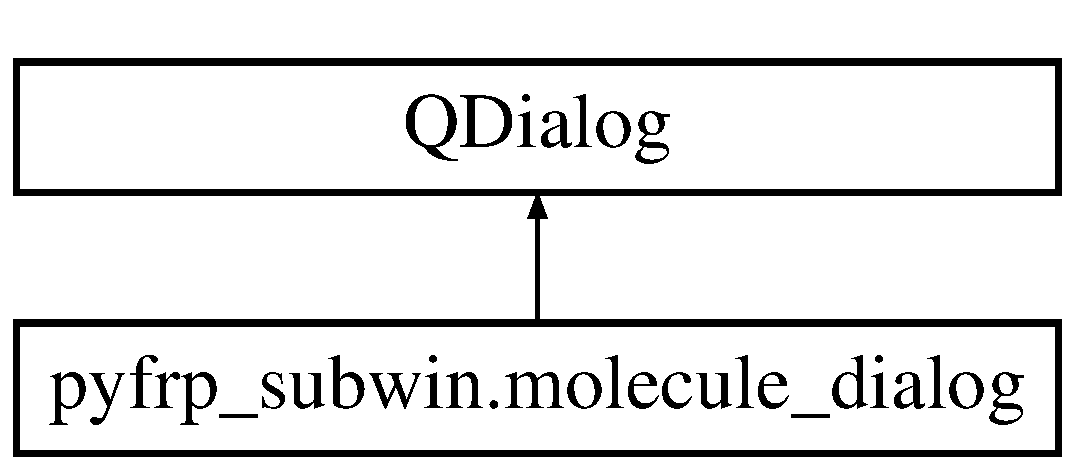
\includegraphics[height=2.000000cm]{classpyfrp__subwin_1_1molecule__dialog}
\end{center}
\end{figure}
\subsection*{Public Member Functions}
\begin{DoxyCompactItemize}
\item 
\hypertarget{classpyfrp__subwin_1_1molecule__dialog_a72d9e9547a32913ef0950df5c2599384}{def {\bfseries \+\_\+\+\_\+init\+\_\+\+\_\+}}\label{classpyfrp__subwin_1_1molecule__dialog_a72d9e9547a32913ef0950df5c2599384}

\item 
\hypertarget{classpyfrp__subwin_1_1molecule__dialog_aab296c6f7bbfc83df4e19d37e53ee49a}{def {\bfseries set\+\_\+name}}\label{classpyfrp__subwin_1_1molecule__dialog_aab296c6f7bbfc83df4e19d37e53ee49a}

\item 
\hypertarget{classpyfrp__subwin_1_1molecule__dialog_a97642425e3f16995acfa9b8ec834cc91}{def {\bfseries done\+\_\+pressed}}\label{classpyfrp__subwin_1_1molecule__dialog_a97642425e3f16995acfa9b8ec834cc91}

\end{DoxyCompactItemize}
\subsection*{Public Attributes}
\begin{DoxyCompactItemize}
\item 
\hypertarget{classpyfrp__subwin_1_1molecule__dialog_ac726a073ac83f2a248c0bc93f2aab33a}{{\bfseries molecule}}\label{classpyfrp__subwin_1_1molecule__dialog_ac726a073ac83f2a248c0bc93f2aab33a}

\item 
\hypertarget{classpyfrp__subwin_1_1molecule__dialog_a0cb1129b780638d4ea04538791ec96ea}{{\bfseries btn\+\_\+done}}\label{classpyfrp__subwin_1_1molecule__dialog_a0cb1129b780638d4ea04538791ec96ea}

\item 
\hypertarget{classpyfrp__subwin_1_1molecule__dialog_acac4040555c3901e2e5973c47ef2aa99}{{\bfseries lbl\+\_\+name}}\label{classpyfrp__subwin_1_1molecule__dialog_acac4040555c3901e2e5973c47ef2aa99}

\item 
\hypertarget{classpyfrp__subwin_1_1molecule__dialog_a2f02990203d941fd588c633e58d03d5d}{{\bfseries qle\+\_\+name}}\label{classpyfrp__subwin_1_1molecule__dialog_a2f02990203d941fd588c633e58d03d5d}

\end{DoxyCompactItemize}


The documentation for this class was generated from the following file\+:\begin{DoxyCompactItemize}
\item 
/home/alex\+\_\+loc/\+Documents/\+Research/\+Py\+F\+R\+A\+P/\+Code/pyfrp\+\_\+subwin.\+py\end{DoxyCompactItemize}

\hypertarget{classpyfrp__subwin_1_1mult__fit__dialog}{\section{pyfrp\+\_\+subwin.\+mult\+\_\+fit\+\_\+dialog Class Reference}
\label{classpyfrp__subwin_1_1mult__fit__dialog}\index{pyfrp\+\_\+subwin.\+mult\+\_\+fit\+\_\+dialog@{pyfrp\+\_\+subwin.\+mult\+\_\+fit\+\_\+dialog}}
}
Inheritance diagram for pyfrp\+\_\+subwin.\+mult\+\_\+fit\+\_\+dialog\+:\begin{figure}[H]
\begin{center}
\leavevmode
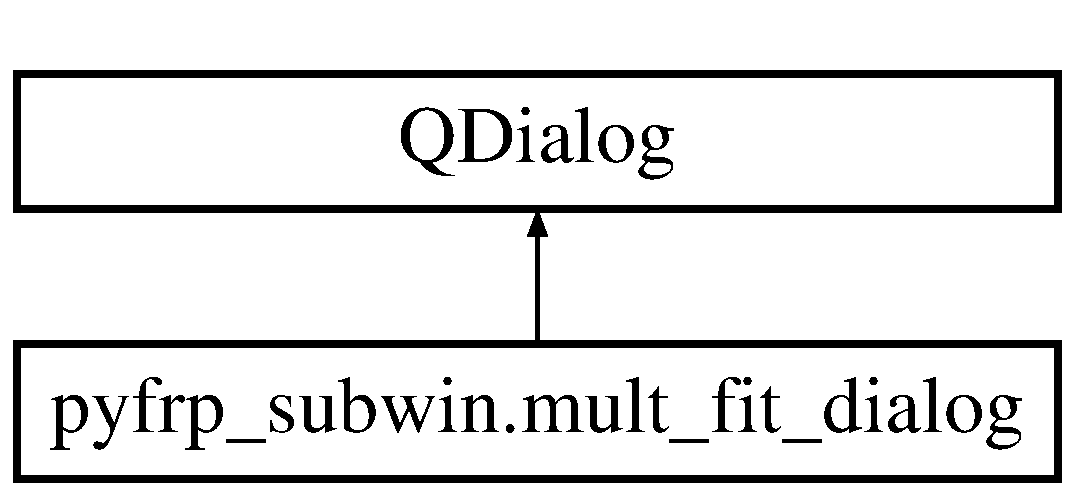
\includegraphics[height=2.000000cm]{classpyfrp__subwin_1_1mult__fit__dialog}
\end{center}
\end{figure}
\subsection*{Public Member Functions}
\begin{DoxyCompactItemize}
\item 
\hypertarget{classpyfrp__subwin_1_1mult__fit__dialog_ae0c1cabf0630351609a48aeba3e171a6}{def {\bfseries \+\_\+\+\_\+init\+\_\+\+\_\+}}\label{classpyfrp__subwin_1_1mult__fit__dialog_ae0c1cabf0630351609a48aeba3e171a6}

\item 
\hypertarget{classpyfrp__subwin_1_1mult__fit__dialog_ad9570ed8145e4d5dbdd9a1e27eafb14d}{def {\bfseries set\+\_\+opt\+\_\+tol}}\label{classpyfrp__subwin_1_1mult__fit__dialog_ad9570ed8145e4d5dbdd9a1e27eafb14d}

\item 
\hypertarget{classpyfrp__subwin_1_1mult__fit__dialog_a5f5baa92741f7f0cc912f425adbaf7f4}{def {\bfseries set\+\_\+maxfun}}\label{classpyfrp__subwin_1_1mult__fit__dialog_a5f5baa92741f7f0cc912f425adbaf7f4}

\item 
\hypertarget{classpyfrp__subwin_1_1mult__fit__dialog_a18dca3ddfcc979dc6ee6958b54fdc8d0}{def {\bfseries set\+\_\+x0\+\_\+\+D}}\label{classpyfrp__subwin_1_1mult__fit__dialog_a18dca3ddfcc979dc6ee6958b54fdc8d0}

\item 
\hypertarget{classpyfrp__subwin_1_1mult__fit__dialog_aee37ed926ae283bd3c36917910aeebe8}{def {\bfseries set\+\_\+x0\+\_\+degr}}\label{classpyfrp__subwin_1_1mult__fit__dialog_aee37ed926ae283bd3c36917910aeebe8}

\item 
\hypertarget{classpyfrp__subwin_1_1mult__fit__dialog_add9cb3874a1bd4ffc6f098a5afddecca}{def {\bfseries set\+\_\+x0\+\_\+prod}}\label{classpyfrp__subwin_1_1mult__fit__dialog_add9cb3874a1bd4ffc6f098a5afddecca}

\item 
\hypertarget{classpyfrp__subwin_1_1mult__fit__dialog_a4b83941b59bb2decfaa11764fc994933}{def {\bfseries set\+\_\+\+U\+B\+\_\+\+D}}\label{classpyfrp__subwin_1_1mult__fit__dialog_a4b83941b59bb2decfaa11764fc994933}

\item 
\hypertarget{classpyfrp__subwin_1_1mult__fit__dialog_a1a32c2164a93d31e639f161dacc4f051}{def {\bfseries set\+\_\+\+U\+B\+\_\+degr}}\label{classpyfrp__subwin_1_1mult__fit__dialog_a1a32c2164a93d31e639f161dacc4f051}

\item 
\hypertarget{classpyfrp__subwin_1_1mult__fit__dialog_a16f533a49ceb1b9a7e5fe6be224f1560}{def {\bfseries set\+\_\+\+U\+B\+\_\+prod}}\label{classpyfrp__subwin_1_1mult__fit__dialog_a16f533a49ceb1b9a7e5fe6be224f1560}

\item 
\hypertarget{classpyfrp__subwin_1_1mult__fit__dialog_a71823526e10603cdbd28e98e9063308e}{def {\bfseries set\+\_\+\+L\+B\+\_\+\+D}}\label{classpyfrp__subwin_1_1mult__fit__dialog_a71823526e10603cdbd28e98e9063308e}

\item 
\hypertarget{classpyfrp__subwin_1_1mult__fit__dialog_a07a44bf22b1bc1c3b2d67075b1e74ee0}{def {\bfseries set\+\_\+\+L\+B\+\_\+degr}}\label{classpyfrp__subwin_1_1mult__fit__dialog_a07a44bf22b1bc1c3b2d67075b1e74ee0}

\item 
\hypertarget{classpyfrp__subwin_1_1mult__fit__dialog_a2f11636b39989f15169a702b519f3bb3}{def {\bfseries set\+\_\+\+L\+B\+\_\+prod}}\label{classpyfrp__subwin_1_1mult__fit__dialog_a2f11636b39989f15169a702b519f3bb3}

\item 
\hypertarget{classpyfrp__subwin_1_1mult__fit__dialog_a87e329d389f68f826fa58a4efeb49801}{def {\bfseries set\+\_\+cut\+\_\+off\+\_\+t}}\label{classpyfrp__subwin_1_1mult__fit__dialog_a87e329d389f68f826fa58a4efeb49801}

\item 
\hypertarget{classpyfrp__subwin_1_1mult__fit__dialog_abd626be0d17280e8438f4d519dcbddfc}{def {\bfseries sel\+\_\+meth}}\label{classpyfrp__subwin_1_1mult__fit__dialog_abd626be0d17280e8438f4d519dcbddfc}

\item 
\hypertarget{classpyfrp__subwin_1_1mult__fit__dialog_a91678a4e6259734c179634adc5bc1caa}{def {\bfseries update\+\_\+bounds\+\_\+after\+\_\+meth}}\label{classpyfrp__subwin_1_1mult__fit__dialog_a91678a4e6259734c179634adc5bc1caa}

\item 
\hypertarget{classpyfrp__subwin_1_1mult__fit__dialog_a109c742e2e2e7320900a968061d90ac0}{def {\bfseries bounds\+\_\+for\+\_\+brute}}\label{classpyfrp__subwin_1_1mult__fit__dialog_a109c742e2e2e7320900a968061d90ac0}

\item 
\hypertarget{classpyfrp__subwin_1_1mult__fit__dialog_a76342a5b7836164c505eab16af676fcf}{def {\bfseries check\+\_\+equ}}\label{classpyfrp__subwin_1_1mult__fit__dialog_a76342a5b7836164c505eab16af676fcf}

\item 
\hypertarget{classpyfrp__subwin_1_1mult__fit__dialog_a04e895152418a2e487f6ebe12ca8b817}{def {\bfseries check\+\_\+pin}}\label{classpyfrp__subwin_1_1mult__fit__dialog_a04e895152418a2e487f6ebe12ca8b817}

\item 
\hypertarget{classpyfrp__subwin_1_1mult__fit__dialog_a5977c93571912bd453972c45bcc3e1d9}{def {\bfseries check\+\_\+cut}}\label{classpyfrp__subwin_1_1mult__fit__dialog_a5977c93571912bd453972c45bcc3e1d9}

\item 
\hypertarget{classpyfrp__subwin_1_1mult__fit__dialog_a03f2528bd9695c27abeb494c9108c339}{def {\bfseries check\+\_\+fit\+\_\+out}}\label{classpyfrp__subwin_1_1mult__fit__dialog_a03f2528bd9695c27abeb494c9108c339}

\item 
\hypertarget{classpyfrp__subwin_1_1mult__fit__dialog_a700da2e2d57c185104c10a3530b23ede}{def {\bfseries check\+\_\+fit\+\_\+slice}}\label{classpyfrp__subwin_1_1mult__fit__dialog_a700da2e2d57c185104c10a3530b23ede}

\item 
\hypertarget{classpyfrp__subwin_1_1mult__fit__dialog_ada8007c32d39d0496a19bc3079224866}{def {\bfseries check\+\_\+fit\+\_\+squ}}\label{classpyfrp__subwin_1_1mult__fit__dialog_ada8007c32d39d0496a19bc3079224866}

\item 
\hypertarget{classpyfrp__subwin_1_1mult__fit__dialog_aa5bda25fcd6d4e345c26af89b5606dcf}{def {\bfseries check\+\_\+fit\+\_\+degr}}\label{classpyfrp__subwin_1_1mult__fit__dialog_aa5bda25fcd6d4e345c26af89b5606dcf}

\item 
\hypertarget{classpyfrp__subwin_1_1mult__fit__dialog_a0659607e3a01468b69556da6f234a980}{def {\bfseries check\+\_\+fit\+\_\+prod}}\label{classpyfrp__subwin_1_1mult__fit__dialog_a0659607e3a01468b69556da6f234a980}

\item 
\hypertarget{classpyfrp__subwin_1_1mult__fit__dialog_adf10cb4f56f56ab16263248e90318a4f}{def {\bfseries check\+\_\+debug\+\_\+fit}}\label{classpyfrp__subwin_1_1mult__fit__dialog_adf10cb4f56f56ab16263248e90318a4f}

\item 
\hypertarget{classpyfrp__subwin_1_1mult__fit__dialog_ab4fdd62aafd43958205ac46af3b46d82}{def {\bfseries check\+\_\+save\+\_\+track}}\label{classpyfrp__subwin_1_1mult__fit__dialog_ab4fdd62aafd43958205ac46af3b46d82}

\item 
\hypertarget{classpyfrp__subwin_1_1mult__fit__dialog_a4def66f7c7d14263b5788e8abd7036c2}{def {\bfseries check\+\_\+bound\+\_\+\+L\+B\+\_\+\+D}}\label{classpyfrp__subwin_1_1mult__fit__dialog_a4def66f7c7d14263b5788e8abd7036c2}

\item 
\hypertarget{classpyfrp__subwin_1_1mult__fit__dialog_a9070a3780b87810480941b18b59f4b22}{def {\bfseries check\+\_\+bound\+\_\+\+U\+B\+\_\+\+D}}\label{classpyfrp__subwin_1_1mult__fit__dialog_a9070a3780b87810480941b18b59f4b22}

\item 
\hypertarget{classpyfrp__subwin_1_1mult__fit__dialog_aa93699ee206f0662dd5268514b3922be}{def {\bfseries check\+\_\+bound\+\_\+\+L\+B\+\_\+degr}}\label{classpyfrp__subwin_1_1mult__fit__dialog_aa93699ee206f0662dd5268514b3922be}

\item 
\hypertarget{classpyfrp__subwin_1_1mult__fit__dialog_a7c53bf4749e328d7a58f5e71314e4731}{def {\bfseries check\+\_\+bound\+\_\+\+U\+B\+\_\+degr}}\label{classpyfrp__subwin_1_1mult__fit__dialog_a7c53bf4749e328d7a58f5e71314e4731}

\item 
\hypertarget{classpyfrp__subwin_1_1mult__fit__dialog_a7f5bf1031f3629724885764c2542fcf7}{def {\bfseries check\+\_\+bound\+\_\+\+L\+B\+\_\+prod}}\label{classpyfrp__subwin_1_1mult__fit__dialog_a7f5bf1031f3629724885764c2542fcf7}

\item 
\hypertarget{classpyfrp__subwin_1_1mult__fit__dialog_acd7751952a7392ab92b44fc9a2888b49}{def {\bfseries check\+\_\+bound\+\_\+\+U\+B\+\_\+prod}}\label{classpyfrp__subwin_1_1mult__fit__dialog_acd7751952a7392ab92b44fc9a2888b49}

\item 
\hypertarget{classpyfrp__subwin_1_1mult__fit__dialog_a3cbaede30dc33581613d5a3b9c420a44}{def {\bfseries done\+\_\+pressed}}\label{classpyfrp__subwin_1_1mult__fit__dialog_a3cbaede30dc33581613d5a3b9c420a44}

\end{DoxyCompactItemize}
\subsection*{Public Attributes}
\begin{DoxyCompactItemize}
\item 
\hypertarget{classpyfrp__subwin_1_1mult__fit__dialog_a04456a0c98d54cab086f4b3f49af4c62}{{\bfseries molecule}}\label{classpyfrp__subwin_1_1mult__fit__dialog_a04456a0c98d54cab086f4b3f49af4c62}

\item 
\hypertarget{classpyfrp__subwin_1_1mult__fit__dialog_a7744257463be627a7ad9d628c7a7d9f2}{{\bfseries temp\+\_\+\+L\+B\+\_\+\+D}}\label{classpyfrp__subwin_1_1mult__fit__dialog_a7744257463be627a7ad9d628c7a7d9f2}

\item 
\hypertarget{classpyfrp__subwin_1_1mult__fit__dialog_a45d0603ddd7f21db1c8d649a4f783814}{{\bfseries temp\+\_\+\+U\+B\+\_\+\+D}}\label{classpyfrp__subwin_1_1mult__fit__dialog_a45d0603ddd7f21db1c8d649a4f783814}

\item 
\hypertarget{classpyfrp__subwin_1_1mult__fit__dialog_afdcee57f4e28deac1556e281b9a95006}{{\bfseries temp\+\_\+\+L\+B\+\_\+degr}}\label{classpyfrp__subwin_1_1mult__fit__dialog_afdcee57f4e28deac1556e281b9a95006}

\item 
\hypertarget{classpyfrp__subwin_1_1mult__fit__dialog_a01d147c5db549d7415d01ba776270cf5}{{\bfseries temp\+\_\+\+U\+B\+\_\+degr}}\label{classpyfrp__subwin_1_1mult__fit__dialog_a01d147c5db549d7415d01ba776270cf5}

\item 
\hypertarget{classpyfrp__subwin_1_1mult__fit__dialog_adb9da4b04752e1af14ddf6339757529e}{{\bfseries temp\+\_\+\+L\+B\+\_\+prod}}\label{classpyfrp__subwin_1_1mult__fit__dialog_adb9da4b04752e1af14ddf6339757529e}

\item 
\hypertarget{classpyfrp__subwin_1_1mult__fit__dialog_a97c021c6c9b087ce4b16c4685ffc5999}{{\bfseries temp\+\_\+\+U\+B\+\_\+prod}}\label{classpyfrp__subwin_1_1mult__fit__dialog_a97c021c6c9b087ce4b16c4685ffc5999}

\item 
\hypertarget{classpyfrp__subwin_1_1mult__fit__dialog_aa7771d147f899d9971e39443a7e73869}{{\bfseries btn\+\_\+done}}\label{classpyfrp__subwin_1_1mult__fit__dialog_aa7771d147f899d9971e39443a7e73869}

\item 
\hypertarget{classpyfrp__subwin_1_1mult__fit__dialog_a78cbd46479f859a84a149ab6017e7a8c}{{\bfseries lbl\+\_\+opt\+\_\+parms}}\label{classpyfrp__subwin_1_1mult__fit__dialog_a78cbd46479f859a84a149ab6017e7a8c}

\item 
\hypertarget{classpyfrp__subwin_1_1mult__fit__dialog_ab0cfb717d80bec3b6db3f3d4220ae768}{{\bfseries lbl\+\_\+guess}}\label{classpyfrp__subwin_1_1mult__fit__dialog_ab0cfb717d80bec3b6db3f3d4220ae768}

\item 
\hypertarget{classpyfrp__subwin_1_1mult__fit__dialog_a59e455d049aafc7457ac38c59cc18dd2}{{\bfseries lbl\+\_\+bounds}}\label{classpyfrp__subwin_1_1mult__fit__dialog_a59e455d049aafc7457ac38c59cc18dd2}

\item 
\hypertarget{classpyfrp__subwin_1_1mult__fit__dialog_ac3c7451b05995d8499447dbea117abdb}{{\bfseries lbl\+\_\+bounded}}\label{classpyfrp__subwin_1_1mult__fit__dialog_ac3c7451b05995d8499447dbea117abdb}

\item 
\hypertarget{classpyfrp__subwin_1_1mult__fit__dialog_ac208ea5ccc9fd9a3b539b63ed553c0f1}{{\bfseries lbl\+\_\+fitting}}\label{classpyfrp__subwin_1_1mult__fit__dialog_ac208ea5ccc9fd9a3b539b63ed553c0f1}

\item 
\hypertarget{classpyfrp__subwin_1_1mult__fit__dialog_ace75235cea2c20bf437398e8dc07b535}{{\bfseries lbl\+\_\+opt\+\_\+meth}}\label{classpyfrp__subwin_1_1mult__fit__dialog_ace75235cea2c20bf437398e8dc07b535}

\item 
\hypertarget{classpyfrp__subwin_1_1mult__fit__dialog_ac8070921271335f84896324882b3ed15}{{\bfseries lbl\+\_\+opt\+\_\+tol}}\label{classpyfrp__subwin_1_1mult__fit__dialog_ac8070921271335f84896324882b3ed15}

\item 
\hypertarget{classpyfrp__subwin_1_1mult__fit__dialog_ab26e8818382042bb60d499e6b2626ae6}{{\bfseries lbl\+\_\+maxfun}}\label{classpyfrp__subwin_1_1mult__fit__dialog_ab26e8818382042bb60d499e6b2626ae6}

\item 
\hypertarget{classpyfrp__subwin_1_1mult__fit__dialog_ae734a81f5c03beb4ecaa8d575f4be136}{{\bfseries lbl\+\_\+save\+\_\+track}}\label{classpyfrp__subwin_1_1mult__fit__dialog_ae734a81f5c03beb4ecaa8d575f4be136}

\item 
\hypertarget{classpyfrp__subwin_1_1mult__fit__dialog_ad5c04e1964963cf3e13e792eb0b5e914}{{\bfseries lbl\+\_\+debug\+\_\+fit}}\label{classpyfrp__subwin_1_1mult__fit__dialog_ad5c04e1964963cf3e13e792eb0b5e914}

\item 
\hypertarget{classpyfrp__subwin_1_1mult__fit__dialog_a084495423a65a3c81ec239f72d4e3015}{{\bfseries lbl\+\_\+x0\+\_\+\+D}}\label{classpyfrp__subwin_1_1mult__fit__dialog_a084495423a65a3c81ec239f72d4e3015}

\item 
\hypertarget{classpyfrp__subwin_1_1mult__fit__dialog_afb179bd9c54b243a62b6c6a59d1db7e4}{{\bfseries lbl\+\_\+x0\+\_\+degr}}\label{classpyfrp__subwin_1_1mult__fit__dialog_afb179bd9c54b243a62b6c6a59d1db7e4}

\item 
\hypertarget{classpyfrp__subwin_1_1mult__fit__dialog_a345caf0e91d27ab2bec2fd11b723433e}{{\bfseries lbl\+\_\+x0\+\_\+prod}}\label{classpyfrp__subwin_1_1mult__fit__dialog_a345caf0e91d27ab2bec2fd11b723433e}

\item 
\hypertarget{classpyfrp__subwin_1_1mult__fit__dialog_ad6fb25d85efd8a457f3b81c6a8a1a4c6}{{\bfseries lbl\+\_\+\+L\+B\+\_\+\+D}}\label{classpyfrp__subwin_1_1mult__fit__dialog_ad6fb25d85efd8a457f3b81c6a8a1a4c6}

\item 
\hypertarget{classpyfrp__subwin_1_1mult__fit__dialog_a77e1a8e177e51558f6b87fc295012538}{{\bfseries lbl\+\_\+\+U\+B\+\_\+\+D}}\label{classpyfrp__subwin_1_1mult__fit__dialog_a77e1a8e177e51558f6b87fc295012538}

\item 
\hypertarget{classpyfrp__subwin_1_1mult__fit__dialog_a39c62b8abf1c7f88ed6047bad9c65a7f}{{\bfseries lbl\+\_\+\+L\+B\+\_\+prod}}\label{classpyfrp__subwin_1_1mult__fit__dialog_a39c62b8abf1c7f88ed6047bad9c65a7f}

\item 
\hypertarget{classpyfrp__subwin_1_1mult__fit__dialog_a04df2ff252aa330179e78f65bf2f9cf6}{{\bfseries lbl\+\_\+\+U\+B\+\_\+prod}}\label{classpyfrp__subwin_1_1mult__fit__dialog_a04df2ff252aa330179e78f65bf2f9cf6}

\item 
\hypertarget{classpyfrp__subwin_1_1mult__fit__dialog_a86e000497514c4a61f26613b880ba16a}{{\bfseries lbl\+\_\+\+L\+B\+\_\+degr}}\label{classpyfrp__subwin_1_1mult__fit__dialog_a86e000497514c4a61f26613b880ba16a}

\item 
\hypertarget{classpyfrp__subwin_1_1mult__fit__dialog_a4fe9c55264f2ea2ee8e6e5f69cc144f4}{{\bfseries lbl\+\_\+\+U\+B\+\_\+degr}}\label{classpyfrp__subwin_1_1mult__fit__dialog_a4fe9c55264f2ea2ee8e6e5f69cc144f4}

\item 
\hypertarget{classpyfrp__subwin_1_1mult__fit__dialog_afde16348df928f807983ced79917a2b7}{{\bfseries lbl\+\_\+fit\+\_\+out}}\label{classpyfrp__subwin_1_1mult__fit__dialog_afde16348df928f807983ced79917a2b7}

\item 
\hypertarget{classpyfrp__subwin_1_1mult__fit__dialog_a07009ebc0c1b80b8b7a1856e8dcdb7ef}{{\bfseries lbl\+\_\+fit\+\_\+squ}}\label{classpyfrp__subwin_1_1mult__fit__dialog_a07009ebc0c1b80b8b7a1856e8dcdb7ef}

\item 
\hypertarget{classpyfrp__subwin_1_1mult__fit__dialog_a01a649b5d16423b65b3d3f57d3441017}{{\bfseries lbl\+\_\+fit\+\_\+slice}}\label{classpyfrp__subwin_1_1mult__fit__dialog_a01a649b5d16423b65b3d3f57d3441017}

\item 
\hypertarget{classpyfrp__subwin_1_1mult__fit__dialog_aa1a6c20c18c40eb734d57decb9943a6b}{{\bfseries lbl\+\_\+fit\+\_\+prod}}\label{classpyfrp__subwin_1_1mult__fit__dialog_aa1a6c20c18c40eb734d57decb9943a6b}

\item 
\hypertarget{classpyfrp__subwin_1_1mult__fit__dialog_a2183f5141d02d5cb60e30aa64a73711a}{{\bfseries lbl\+\_\+fit\+\_\+degr}}\label{classpyfrp__subwin_1_1mult__fit__dialog_a2183f5141d02d5cb60e30aa64a73711a}

\item 
\hypertarget{classpyfrp__subwin_1_1mult__fit__dialog_ae02c20d45243afad42fad92b43df7c70}{{\bfseries lbl\+\_\+eq}}\label{classpyfrp__subwin_1_1mult__fit__dialog_ae02c20d45243afad42fad92b43df7c70}

\item 
\hypertarget{classpyfrp__subwin_1_1mult__fit__dialog_a55979b31507f606c4a5f9f4b995a211e}{{\bfseries lbl\+\_\+pin}}\label{classpyfrp__subwin_1_1mult__fit__dialog_a55979b31507f606c4a5f9f4b995a211e}

\item 
\hypertarget{classpyfrp__subwin_1_1mult__fit__dialog_a76b12c913aec2a2be266ebe58494a52d}{{\bfseries lbl\+\_\+cut\+\_\+off}}\label{classpyfrp__subwin_1_1mult__fit__dialog_a76b12c913aec2a2be266ebe58494a52d}

\item 
\hypertarget{classpyfrp__subwin_1_1mult__fit__dialog_a1162608be8fcd26347894fde87e57672}{{\bfseries lbl\+\_\+cut\+\_\+off\+\_\+t}}\label{classpyfrp__subwin_1_1mult__fit__dialog_a1162608be8fcd26347894fde87e57672}

\item 
\hypertarget{classpyfrp__subwin_1_1mult__fit__dialog_a4a12107669c932553a7ad9aaf9651eac}{{\bfseries combo\+\_\+meth}}\label{classpyfrp__subwin_1_1mult__fit__dialog_a4a12107669c932553a7ad9aaf9651eac}

\item 
\hypertarget{classpyfrp__subwin_1_1mult__fit__dialog_a46a575723bf1808982733d1f81f31318}{{\bfseries qle\+\_\+opt\+\_\+tol}}\label{classpyfrp__subwin_1_1mult__fit__dialog_a46a575723bf1808982733d1f81f31318}

\item 
\hypertarget{classpyfrp__subwin_1_1mult__fit__dialog_a9aeb7b5e5fdb30c9b3ddf156a2775fb0}{{\bfseries qle\+\_\+maxfun}}\label{classpyfrp__subwin_1_1mult__fit__dialog_a9aeb7b5e5fdb30c9b3ddf156a2775fb0}

\item 
\hypertarget{classpyfrp__subwin_1_1mult__fit__dialog_a40350b97b8ff2ab3178064bb5f79cdc6}{{\bfseries qle\+\_\+x0\+\_\+\+D}}\label{classpyfrp__subwin_1_1mult__fit__dialog_a40350b97b8ff2ab3178064bb5f79cdc6}

\item 
\hypertarget{classpyfrp__subwin_1_1mult__fit__dialog_a201a8bbef3f2a708b72aaee7491cd91b}{{\bfseries qle\+\_\+x0\+\_\+degr}}\label{classpyfrp__subwin_1_1mult__fit__dialog_a201a8bbef3f2a708b72aaee7491cd91b}

\item 
\hypertarget{classpyfrp__subwin_1_1mult__fit__dialog_a29b0cf09dfe74b2ad25c8eac67a94330}{{\bfseries qle\+\_\+x0\+\_\+prod}}\label{classpyfrp__subwin_1_1mult__fit__dialog_a29b0cf09dfe74b2ad25c8eac67a94330}

\item 
\hypertarget{classpyfrp__subwin_1_1mult__fit__dialog_adbcf1e6d4d09d75d91a4d678034a2306}{{\bfseries qle\+\_\+cut\+\_\+off\+\_\+t}}\label{classpyfrp__subwin_1_1mult__fit__dialog_adbcf1e6d4d09d75d91a4d678034a2306}

\item 
\hypertarget{classpyfrp__subwin_1_1mult__fit__dialog_a540121de7aa5b69b9b826f3c7e4bec32}{{\bfseries qle\+\_\+\+L\+B\+\_\+\+D}}\label{classpyfrp__subwin_1_1mult__fit__dialog_a540121de7aa5b69b9b826f3c7e4bec32}

\item 
\hypertarget{classpyfrp__subwin_1_1mult__fit__dialog_a9e7462451412d5084ca378a398ac1957}{{\bfseries qle\+\_\+\+U\+B\+\_\+\+D}}\label{classpyfrp__subwin_1_1mult__fit__dialog_a9e7462451412d5084ca378a398ac1957}

\item 
\hypertarget{classpyfrp__subwin_1_1mult__fit__dialog_a3c053ed05e08c7e44ddfb7d099606dfe}{{\bfseries qle\+\_\+\+L\+B\+\_\+degr}}\label{classpyfrp__subwin_1_1mult__fit__dialog_a3c053ed05e08c7e44ddfb7d099606dfe}

\item 
\hypertarget{classpyfrp__subwin_1_1mult__fit__dialog_acbbf12564f62caecc74bcb15d10e1934}{{\bfseries qle\+\_\+\+U\+B\+\_\+degr}}\label{classpyfrp__subwin_1_1mult__fit__dialog_acbbf12564f62caecc74bcb15d10e1934}

\item 
\hypertarget{classpyfrp__subwin_1_1mult__fit__dialog_ac024709e712485dc0bf4b81a850ffaf3}{{\bfseries qle\+\_\+\+L\+B\+\_\+prod}}\label{classpyfrp__subwin_1_1mult__fit__dialog_ac024709e712485dc0bf4b81a850ffaf3}

\item 
\hypertarget{classpyfrp__subwin_1_1mult__fit__dialog_a8ada450c2cb182977b73e8a12b3d62ad}{{\bfseries qle\+\_\+\+U\+B\+\_\+prod}}\label{classpyfrp__subwin_1_1mult__fit__dialog_a8ada450c2cb182977b73e8a12b3d62ad}

\item 
\hypertarget{classpyfrp__subwin_1_1mult__fit__dialog_a8ffab30b67a6f04e4e143e007e444461}{{\bfseries double\+\_\+valid}}\label{classpyfrp__subwin_1_1mult__fit__dialog_a8ffab30b67a6f04e4e143e007e444461}

\item 
\hypertarget{classpyfrp__subwin_1_1mult__fit__dialog_a2dc9b34dee72ea6dd2df49ced6f9a7a7}{{\bfseries cb\+\_\+debug\+\_\+fit}}\label{classpyfrp__subwin_1_1mult__fit__dialog_a2dc9b34dee72ea6dd2df49ced6f9a7a7}

\item 
\hypertarget{classpyfrp__subwin_1_1mult__fit__dialog_ac135cebab0c04931cabcf0906f3814a8}{{\bfseries cb\+\_\+save\+\_\+track}}\label{classpyfrp__subwin_1_1mult__fit__dialog_ac135cebab0c04931cabcf0906f3814a8}

\item 
\hypertarget{classpyfrp__subwin_1_1mult__fit__dialog_ae53fa7defe721ff1dc25e437e41e9748}{{\bfseries cb\+\_\+bound\+\_\+\+L\+B\+\_\+\+D}}\label{classpyfrp__subwin_1_1mult__fit__dialog_ae53fa7defe721ff1dc25e437e41e9748}

\item 
\hypertarget{classpyfrp__subwin_1_1mult__fit__dialog_ad6d0f86a155d02fbda97b58c343e09f5}{{\bfseries cb\+\_\+bound\+\_\+\+L\+B\+\_\+degr}}\label{classpyfrp__subwin_1_1mult__fit__dialog_ad6d0f86a155d02fbda97b58c343e09f5}

\item 
\hypertarget{classpyfrp__subwin_1_1mult__fit__dialog_a3a691c7fde1bf110402a19a4824b809c}{{\bfseries cb\+\_\+bound\+\_\+\+L\+B\+\_\+prod}}\label{classpyfrp__subwin_1_1mult__fit__dialog_a3a691c7fde1bf110402a19a4824b809c}

\item 
\hypertarget{classpyfrp__subwin_1_1mult__fit__dialog_a11a1eed3df67194758fca527052785be}{{\bfseries cb\+\_\+bound\+\_\+\+U\+B\+\_\+\+D}}\label{classpyfrp__subwin_1_1mult__fit__dialog_a11a1eed3df67194758fca527052785be}

\item 
\hypertarget{classpyfrp__subwin_1_1mult__fit__dialog_a74c0e9c10d112203c7bd9046b65a23e1}{{\bfseries cb\+\_\+bound\+\_\+\+U\+B\+\_\+degr}}\label{classpyfrp__subwin_1_1mult__fit__dialog_a74c0e9c10d112203c7bd9046b65a23e1}

\item 
\hypertarget{classpyfrp__subwin_1_1mult__fit__dialog_a09c2ebbebb18178b2d3bb84e741a5c98}{{\bfseries cb\+\_\+bound\+\_\+\+U\+B\+\_\+prod}}\label{classpyfrp__subwin_1_1mult__fit__dialog_a09c2ebbebb18178b2d3bb84e741a5c98}

\item 
\hypertarget{classpyfrp__subwin_1_1mult__fit__dialog_a0525c684fb30917a4cf20fc5195f4336}{{\bfseries cb\+\_\+fit\+\_\+out}}\label{classpyfrp__subwin_1_1mult__fit__dialog_a0525c684fb30917a4cf20fc5195f4336}

\item 
\hypertarget{classpyfrp__subwin_1_1mult__fit__dialog_abca8f083de1d650ed3c3702918a25c22}{{\bfseries cb\+\_\+fit\+\_\+squ}}\label{classpyfrp__subwin_1_1mult__fit__dialog_abca8f083de1d650ed3c3702918a25c22}

\item 
\hypertarget{classpyfrp__subwin_1_1mult__fit__dialog_ae542f31bc0b9d4ac37a74952ddf39546}{{\bfseries cb\+\_\+fit\+\_\+slice}}\label{classpyfrp__subwin_1_1mult__fit__dialog_ae542f31bc0b9d4ac37a74952ddf39546}

\item 
\hypertarget{classpyfrp__subwin_1_1mult__fit__dialog_ab84801cab2aa0929cbd29d3eff44c01e}{{\bfseries cb\+\_\+fit\+\_\+degr}}\label{classpyfrp__subwin_1_1mult__fit__dialog_ab84801cab2aa0929cbd29d3eff44c01e}

\item 
\hypertarget{classpyfrp__subwin_1_1mult__fit__dialog_a49af28a0d8538d3a128bddaae24df611}{{\bfseries cb\+\_\+fit\+\_\+prod}}\label{classpyfrp__subwin_1_1mult__fit__dialog_a49af28a0d8538d3a128bddaae24df611}

\item 
\hypertarget{classpyfrp__subwin_1_1mult__fit__dialog_ab82669683058de548f19a958a60d2d62}{{\bfseries cb\+\_\+eq}}\label{classpyfrp__subwin_1_1mult__fit__dialog_ab82669683058de548f19a958a60d2d62}

\item 
\hypertarget{classpyfrp__subwin_1_1mult__fit__dialog_a4b9a74fbe7990ba9b8870a8f94a82d3d}{{\bfseries cb\+\_\+pin}}\label{classpyfrp__subwin_1_1mult__fit__dialog_a4b9a74fbe7990ba9b8870a8f94a82d3d}

\item 
\hypertarget{classpyfrp__subwin_1_1mult__fit__dialog_a4dda96634c255ea9149c2a98ec7778d4}{{\bfseries cb\+\_\+cut}}\label{classpyfrp__subwin_1_1mult__fit__dialog_a4dda96634c255ea9149c2a98ec7778d4}

\end{DoxyCompactItemize}


The documentation for this class was generated from the following file\+:\begin{DoxyCompactItemize}
\item 
/home/alex\+\_\+loc/\+Documents/\+Research/\+Py\+F\+R\+A\+P/\+Code/pyfrp\+\_\+subwin.\+py\end{DoxyCompactItemize}

\hypertarget{classpyfrp__app_1_1pyfrp}{\section{pyfrp\+\_\+app.\+pyfrp Class Reference}
\label{classpyfrp__app_1_1pyfrp}\index{pyfrp\+\_\+app.\+pyfrp@{pyfrp\+\_\+app.\+pyfrp}}
}
Inheritance diagram for pyfrp\+\_\+app.\+pyfrp\+:\begin{figure}[H]
\begin{center}
\leavevmode
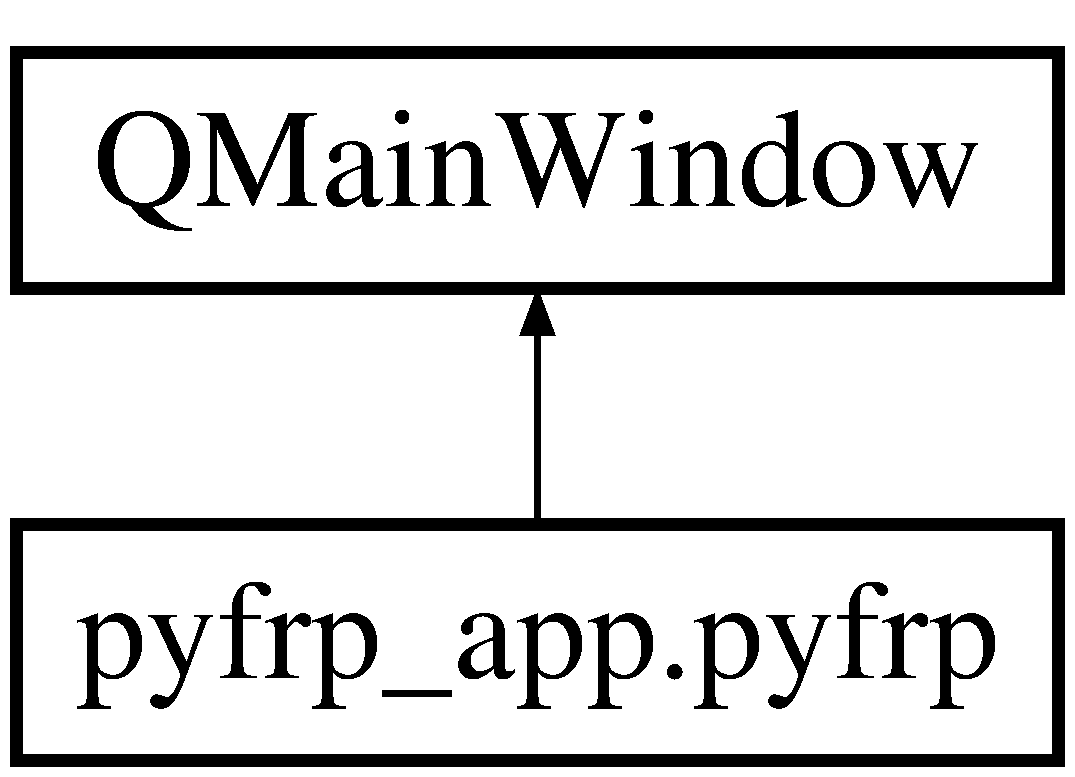
\includegraphics[height=2.000000cm]{classpyfrp__app_1_1pyfrp}
\end{center}
\end{figure}
\subsection*{Public Member Functions}
\begin{DoxyCompactItemize}
\item 
\hypertarget{classpyfrp__app_1_1pyfrp_a45c2b5c7d4f88bb20a4ceabe900d9a86}{def {\bfseries \+\_\+\+\_\+init\+\_\+\+\_\+}}\label{classpyfrp__app_1_1pyfrp_a45c2b5c7d4f88bb20a4ceabe900d9a86}

\item 
\hypertarget{classpyfrp__app_1_1pyfrp_a3f937942f2e64f0676f3a86da48f19ea}{def {\bfseries close\+Event}}\label{classpyfrp__app_1_1pyfrp_a3f937942f2e64f0676f3a86da48f19ea}

\item 
\hypertarget{classpyfrp__app_1_1pyfrp_a2399d8c9e71409db81443b3f38172443}{def {\bfseries show\+\_\+about}}\label{classpyfrp__app_1_1pyfrp_a2399d8c9e71409db81443b3f38172443}

\item 
\hypertarget{classpyfrp__app_1_1pyfrp_a3f8f06392e2b13b1c7ce11d4e36dccac}{def {\bfseries create\+\_\+frame}}\label{classpyfrp__app_1_1pyfrp_a3f8f06392e2b13b1c7ce11d4e36dccac}

\item 
\hypertarget{classpyfrp__app_1_1pyfrp_ab073245b66a0f4e5a1f64d6fb302a4a3}{def {\bfseries init\+\_\+conf}}\label{classpyfrp__app_1_1pyfrp_ab073245b66a0f4e5a1f64d6fb302a4a3}

\item 
\hypertarget{classpyfrp__app_1_1pyfrp_a82d010d3eb0ec3efc397f5b8e8cc620a}{def {\bfseries append\+\_\+recent}}\label{classpyfrp__app_1_1pyfrp_a82d010d3eb0ec3efc397f5b8e8cc620a}

\item 
\hypertarget{classpyfrp__app_1_1pyfrp_ac658e2ddb4241674112e99356da2f04c}{def {\bfseries add\+\_\+recent\+\_\+mbs}}\label{classpyfrp__app_1_1pyfrp_ac658e2ddb4241674112e99356da2f04c}

\item 
\hypertarget{classpyfrp__app_1_1pyfrp_a5d34580abe8086a99c4580821610f7d8}{def {\bfseries add\+\_\+molecule}}\label{classpyfrp__app_1_1pyfrp_a5d34580abe8086a99c4580821610f7d8}

\item 
\hypertarget{classpyfrp__app_1_1pyfrp_a76e1016a9cbde9f1cd49c98ffee6ae62}{def {\bfseries add\+\_\+embryo}}\label{classpyfrp__app_1_1pyfrp_a76e1016a9cbde9f1cd49c98ffee6ae62}

\item 
\hypertarget{classpyfrp__app_1_1pyfrp_ae0d4c8e623cdcd633d85be0195fd157f}{def {\bfseries delete\+\_\+molecule}}\label{classpyfrp__app_1_1pyfrp_ae0d4c8e623cdcd633d85be0195fd157f}

\item 
\hypertarget{classpyfrp__app_1_1pyfrp_ad486b9dceb8db3ce73e2f127d21927bc}{def {\bfseries delete\+\_\+embryo}}\label{classpyfrp__app_1_1pyfrp_ad486b9dceb8db3ce73e2f127d21927bc}

\item 
\hypertarget{classpyfrp__app_1_1pyfrp_a9b10e0ba6db57a0df4999e7d99b25386}{def {\bfseries delete\+\_\+specific\+\_\+molecule}}\label{classpyfrp__app_1_1pyfrp_a9b10e0ba6db57a0df4999e7d99b25386}

\item 
\hypertarget{classpyfrp__app_1_1pyfrp_a2c451b320d1fcfcf1a5f5c3b43984938}{def {\bfseries delete\+\_\+specific\+\_\+embryo}}\label{classpyfrp__app_1_1pyfrp_a2c451b320d1fcfcf1a5f5c3b43984938}

\item 
\hypertarget{classpyfrp__app_1_1pyfrp_abb63044d4d4cce042c8f18fd69169359}{def {\bfseries save\+\_\+molecule}}\label{classpyfrp__app_1_1pyfrp_abb63044d4d4cce042c8f18fd69169359}

\item 
\hypertarget{classpyfrp__app_1_1pyfrp_aa070886230c00bf7d27ac95366efa3b2}{def {\bfseries save\+\_\+embryo}}\label{classpyfrp__app_1_1pyfrp_aa070886230c00bf7d27ac95366efa3b2}

\item 
\hypertarget{classpyfrp__app_1_1pyfrp_afc040c7fb984d046fea9d364f8cafeae}{def {\bfseries load\+\_\+molecule}}\label{classpyfrp__app_1_1pyfrp_afc040c7fb984d046fea9d364f8cafeae}

\item 
\hypertarget{classpyfrp__app_1_1pyfrp_a1877c3dcdb35faaef85feed8028c4224}{def {\bfseries open\+\_\+molecule}}\label{classpyfrp__app_1_1pyfrp_a1877c3dcdb35faaef85feed8028c4224}

\item 
\hypertarget{classpyfrp__app_1_1pyfrp_aa5dc6678a25931014a488c6594567ef0}{def {\bfseries load\+\_\+embryo}}\label{classpyfrp__app_1_1pyfrp_aa5dc6678a25931014a488c6594567ef0}

\item 
\hypertarget{classpyfrp__app_1_1pyfrp_ab885b0d956570b8f600e2b2e2b46a815}{def {\bfseries show\+\_\+embryo\+\_\+props}}\label{classpyfrp__app_1_1pyfrp_ab885b0d956570b8f600e2b2e2b46a815}

\item 
\hypertarget{classpyfrp__app_1_1pyfrp_ae1a22a77faee45c1d82e524dc3708027}{def {\bfseries add\+\_\+fit}}\label{classpyfrp__app_1_1pyfrp_ae1a22a77faee45c1d82e524dc3708027}

\item 
\hypertarget{classpyfrp__app_1_1pyfrp_acea292c4e07bd8fcc5aae84ed15935ee}{def {\bfseries copy\+\_\+fit}}\label{classpyfrp__app_1_1pyfrp_acea292c4e07bd8fcc5aae84ed15935ee}

\item 
\hypertarget{classpyfrp__app_1_1pyfrp_ab8dbdc18ca6d1bd0e42fc245592c82c8}{def {\bfseries copy\+\_\+fit\+\_\+for\+\_\+other\+\_\+embryo}}\label{classpyfrp__app_1_1pyfrp_ab8dbdc18ca6d1bd0e42fc245592c82c8}

\item 
\hypertarget{classpyfrp__app_1_1pyfrp_a0ab36bf82bf97cc39fd31fd125cf6af0}{def {\bfseries copy\+\_\+fit\+\_\+to\+\_\+all}}\label{classpyfrp__app_1_1pyfrp_a0ab36bf82bf97cc39fd31fd125cf6af0}

\item 
\hypertarget{classpyfrp__app_1_1pyfrp_a67d94f915751de406116114a30be907b}{def {\bfseries delete\+\_\+fit}}\label{classpyfrp__app_1_1pyfrp_a67d94f915751de406116114a30be907b}

\item 
\hypertarget{classpyfrp__app_1_1pyfrp_a76c29d1c1ef4f97a471f8da4983fc9bb}{def {\bfseries edit\+\_\+fit}}\label{classpyfrp__app_1_1pyfrp_a76c29d1c1ef4f97a471f8da4983fc9bb}

\item 
\hypertarget{classpyfrp__app_1_1pyfrp_ac7cfceccd48317ffe036e0b7d2f3f0af}{def {\bfseries edit\+\_\+mult\+\_\+fit}}\label{classpyfrp__app_1_1pyfrp_ac7cfceccd48317ffe036e0b7d2f3f0af}

\item 
\hypertarget{classpyfrp__app_1_1pyfrp_a40261883602ef8912b0e87f1ed7f1879}{def {\bfseries edit\+\_\+dataset}}\label{classpyfrp__app_1_1pyfrp_a40261883602ef8912b0e87f1ed7f1879}

\item 
\hypertarget{classpyfrp__app_1_1pyfrp_acc0c8932467565dc76f39ba9385ddedf}{def {\bfseries edit\+\_\+molecule}}\label{classpyfrp__app_1_1pyfrp_acc0c8932467565dc76f39ba9385ddedf}

\item 
\hypertarget{classpyfrp__app_1_1pyfrp_a93922af0c493f95217dfb4dcfa9166bd}{def {\bfseries copy\+\_\+embryo}}\label{classpyfrp__app_1_1pyfrp_a93922af0c493f95217dfb4dcfa9166bd}

\item 
\hypertarget{classpyfrp__app_1_1pyfrp_a4a29599b8b8ff030952f5e5ab0b363e0}{def {\bfseries copy\+\_\+molecule}}\label{classpyfrp__app_1_1pyfrp_a4a29599b8b8ff030952f5e5ab0b363e0}

\item 
\hypertarget{classpyfrp__app_1_1pyfrp_abda151732bfadd14d05831dae9a95ffb}{def {\bfseries edit\+\_\+prop}}\label{classpyfrp__app_1_1pyfrp_abda151732bfadd14d05831dae9a95ffb}

\item 
\hypertarget{classpyfrp__app_1_1pyfrp_ae92b16c063808c0c0b8c70270d8cb693}{def {\bfseries analyze\+\_\+all}}\label{classpyfrp__app_1_1pyfrp_ae92b16c063808c0c0b8c70270d8cb693}

\item 
\hypertarget{classpyfrp__app_1_1pyfrp_ad377e093609dfdcdf1c670eb94fc68a6}{def {\bfseries analyze\+\_\+all\+\_\+print\+\_\+prog}}\label{classpyfrp__app_1_1pyfrp_ad377e093609dfdcdf1c670eb94fc68a6}

\item 
\hypertarget{classpyfrp__app_1_1pyfrp_adaa5e5460d453a0c5cf945e66acfb811}{def {\bfseries analyze\+\_\+all\+\_\+finished}}\label{classpyfrp__app_1_1pyfrp_adaa5e5460d453a0c5cf945e66acfb811}

\item 
\hypertarget{classpyfrp__app_1_1pyfrp_af3f239b3c783222be00842ad6195da90}{def {\bfseries analyze\+\_\+all\+\_\+canceled}}\label{classpyfrp__app_1_1pyfrp_af3f239b3c783222be00842ad6195da90}

\item 
\hypertarget{classpyfrp__app_1_1pyfrp_aeecc257fc2e6d7663493740ca559468c}{def {\bfseries analyze\+\_\+dataset}}\label{classpyfrp__app_1_1pyfrp_aeecc257fc2e6d7663493740ca559468c}

\item 
\hypertarget{classpyfrp__app_1_1pyfrp_a0e60a19de87ece53cbdd1b9e4d0edc1e}{def {\bfseries analyze\+\_\+print\+\_\+prog}}\label{classpyfrp__app_1_1pyfrp_a0e60a19de87ece53cbdd1b9e4d0edc1e}

\item 
\hypertarget{classpyfrp__app_1_1pyfrp_a36a92856cb2d01f3422210a6c5cd6972}{def {\bfseries analyze\+\_\+finished}}\label{classpyfrp__app_1_1pyfrp_a36a92856cb2d01f3422210a6c5cd6972}

\item 
\hypertarget{classpyfrp__app_1_1pyfrp_a1b7659127d0e452956778d8c8002a3b3}{def {\bfseries analyze\+\_\+canceled}}\label{classpyfrp__app_1_1pyfrp_a1b7659127d0e452956778d8c8002a3b3}

\item 
\hypertarget{classpyfrp__app_1_1pyfrp_a3406654822e228b68f0fc041ef249cb1}{def {\bfseries edit\+\_\+geometry}}\label{classpyfrp__app_1_1pyfrp_a3406654822e228b68f0fc041ef249cb1}

\item 
\hypertarget{classpyfrp__app_1_1pyfrp_a6fb872ed6beec7df79f4dc00dd73bf9c}{def {\bfseries edit\+\_\+pde\+\_\+parms}}\label{classpyfrp__app_1_1pyfrp_a6fb872ed6beec7df79f4dc00dd73bf9c}

\item 
\hypertarget{classpyfrp__app_1_1pyfrp_ab39dafe885ba886bb3549fdaf2970019}{def {\bfseries simulate\+\_\+embryo}}\label{classpyfrp__app_1_1pyfrp_ab39dafe885ba886bb3549fdaf2970019}

\item 
\hypertarget{classpyfrp__app_1_1pyfrp_a2dff24aaaa48b7f495677f68e00fe9a4}{def {\bfseries simulation\+\_\+print\+\_\+prog}}\label{classpyfrp__app_1_1pyfrp_a2dff24aaaa48b7f495677f68e00fe9a4}

\item 
\hypertarget{classpyfrp__app_1_1pyfrp_a551456911df89cf21707e4f8b82e4644}{def {\bfseries simulation\+\_\+finished}}\label{classpyfrp__app_1_1pyfrp_a551456911df89cf21707e4f8b82e4644}

\item 
\hypertarget{classpyfrp__app_1_1pyfrp_ac032f12dfbd4d58f422a7267ee74d42a}{def {\bfseries simulation\+\_\+canceled}}\label{classpyfrp__app_1_1pyfrp_ac032f12dfbd4d58f422a7267ee74d42a}

\item 
\hypertarget{classpyfrp__app_1_1pyfrp_affaed76f322af4ba52f4357d174f30d1}{def {\bfseries plot\+\_\+data\+\_\+timeseries}}\label{classpyfrp__app_1_1pyfrp_affaed76f322af4ba52f4357d174f30d1}

\item 
\hypertarget{classpyfrp__app_1_1pyfrp_ac3142c727a6572ba9a9b3703cd31f908}{def {\bfseries plot\+\_\+sim\+\_\+timeseries}}\label{classpyfrp__app_1_1pyfrp_ac3142c727a6572ba9a9b3703cd31f908}

\item 
\hypertarget{classpyfrp__app_1_1pyfrp_a79476038a642529615774c40930c03df}{def {\bfseries plot\+\_\+sim\+\_\+data\+\_\+timeseries}}\label{classpyfrp__app_1_1pyfrp_a79476038a642529615774c40930c03df}

\item 
\hypertarget{classpyfrp__app_1_1pyfrp_aa00a3751f18efa9b1b494323b9de9375}{def {\bfseries plot\+\_\+embryo\+\_\+slice\+\_\+imgs}}\label{classpyfrp__app_1_1pyfrp_aa00a3751f18efa9b1b494323b9de9375}

\item 
\hypertarget{classpyfrp__app_1_1pyfrp_a365cae6716e83b0c5237bc289ab05e75}{def {\bfseries plot\+\_\+embryo\+\_\+ext\+\_\+imgs}}\label{classpyfrp__app_1_1pyfrp_a365cae6716e83b0c5237bc289ab05e75}

\item 
\hypertarget{classpyfrp__app_1_1pyfrp_a07843e0bed9441ae0cf9631c2461bcba}{def {\bfseries plot\+\_\+embryo\+\_\+int\+\_\+imgs}}\label{classpyfrp__app_1_1pyfrp_a07843e0bed9441ae0cf9631c2461bcba}

\item 
\hypertarget{classpyfrp__app_1_1pyfrp_a91413c0143c9157fbed3b977d28a187c}{def {\bfseries plot\+\_\+embryo\+\_\+masks\+\_\+embryo}}\label{classpyfrp__app_1_1pyfrp_a91413c0143c9157fbed3b977d28a187c}

\item 
\hypertarget{classpyfrp__app_1_1pyfrp_a8e2a04056fc91691f23dd6595720986e}{def {\bfseries plot\+\_\+embryo\+\_\+masks\+\_\+ext}}\label{classpyfrp__app_1_1pyfrp_a8e2a04056fc91691f23dd6595720986e}

\item 
\hypertarget{classpyfrp__app_1_1pyfrp_afe9795fa06bc25f59547459a9cb02ce3}{def {\bfseries plot\+\_\+embryo\+\_\+masks\+\_\+int}}\label{classpyfrp__app_1_1pyfrp_afe9795fa06bc25f59547459a9cb02ce3}

\item 
\hypertarget{classpyfrp__app_1_1pyfrp_a4de71d2fa08858feab6f4532c04fc9a3}{def {\bfseries plot\+\_\+embryo\+\_\+img\+\_\+series}}\label{classpyfrp__app_1_1pyfrp_a4de71d2fa08858feab6f4532c04fc9a3}

\item 
\hypertarget{classpyfrp__app_1_1pyfrp_ab5a900276d972d608e14aa33ef5e14ac}{def {\bfseries plot\+\_\+fit}}\label{classpyfrp__app_1_1pyfrp_ab5a900276d972d608e14aa33ef5e14ac}

\item 
\hypertarget{classpyfrp__app_1_1pyfrp_ab3e658a027990e5cc6eb2b362800cc29}{def {\bfseries plot\+\_\+track\+\_\+fit}}\label{classpyfrp__app_1_1pyfrp_ab3e658a027990e5cc6eb2b362800cc29}

\item 
\hypertarget{classpyfrp__app_1_1pyfrp_a101613abaf90ecc3219795c1dee960df}{def {\bfseries create\+\_\+plot\+\_\+tab}}\label{classpyfrp__app_1_1pyfrp_a101613abaf90ecc3219795c1dee960df}

\item 
\hypertarget{classpyfrp__app_1_1pyfrp_ac5155d9cad2df02d9456aa3fa3558381}{def {\bfseries curr\+\_\+tab\+\_\+changed}}\label{classpyfrp__app_1_1pyfrp_ac5155d9cad2df02d9456aa3fa3558381}

\item 
\hypertarget{classpyfrp__app_1_1pyfrp_a0ebaf0772cb2464eec539f2206e8fe84}{def {\bfseries curr\+\_\+tab\+\_\+closed}}\label{classpyfrp__app_1_1pyfrp_a0ebaf0772cb2464eec539f2206e8fe84}

\item 
\hypertarget{classpyfrp__app_1_1pyfrp_af044fb6886ad08dad1e27b38e9d53a14}{def {\bfseries adjust\+\_\+canvas}}\label{classpyfrp__app_1_1pyfrp_af044fb6886ad08dad1e27b38e9d53a14}

\item 
\hypertarget{classpyfrp__app_1_1pyfrp_a91b5949ff7cb6b826e0281a9cb9e243d}{def {\bfseries create\+\_\+slider\+\_\+plot\+\_\+tab}}\label{classpyfrp__app_1_1pyfrp_a91b5949ff7cb6b826e0281a9cb9e243d}

\item 
\hypertarget{classpyfrp__app_1_1pyfrp_a34028e31ec48f13ecfd93cf2bfe88c47}{def {\bfseries update\+\_\+slider\+\_\+bkgd}}\label{classpyfrp__app_1_1pyfrp_a34028e31ec48f13ecfd93cf2bfe88c47}

\item 
\hypertarget{classpyfrp__app_1_1pyfrp_a56bb4d3baba87fff8158903b317673d1}{def {\bfseries update\+\_\+slider\+\_\+track}}\label{classpyfrp__app_1_1pyfrp_a56bb4d3baba87fff8158903b317673d1}

\item 
\hypertarget{classpyfrp__app_1_1pyfrp_a43f4d7de3572c061d9ae5e23709f24a9}{def {\bfseries perform\+\_\+fit}}\label{classpyfrp__app_1_1pyfrp_a43f4d7de3572c061d9ae5e23709f24a9}

\item 
\hypertarget{classpyfrp__app_1_1pyfrp_aed48fe21102e91ea83765a3b7df8499b}{def {\bfseries fitting\+\_\+finished}}\label{classpyfrp__app_1_1pyfrp_aed48fe21102e91ea83765a3b7df8499b}

\item 
\hypertarget{classpyfrp__app_1_1pyfrp_a6000c578d68b5838e032727ab6410ef3}{def {\bfseries fitting\+\_\+canceled}}\label{classpyfrp__app_1_1pyfrp_a6000c578d68b5838e032727ab6410ef3}

\item 
\hypertarget{classpyfrp__app_1_1pyfrp_a2fdb089e9afcd350231afa30ca7a3583}{def {\bfseries perform\+\_\+fits\+\_\+molecule}}\label{classpyfrp__app_1_1pyfrp_a2fdb089e9afcd350231afa30ca7a3583}

\item 
\hypertarget{classpyfrp__app_1_1pyfrp_a184b6597fc53ec0690ec9b4e97579f41}{def {\bfseries fitting\+\_\+all\+\_\+finished}}\label{classpyfrp__app_1_1pyfrp_a184b6597fc53ec0690ec9b4e97579f41}

\item 
\hypertarget{classpyfrp__app_1_1pyfrp_ad7df05abde3e5251c0b78a34241b4417}{def {\bfseries show\+\_\+console}}\label{classpyfrp__app_1_1pyfrp_ad7df05abde3e5251c0b78a34241b4417}

\item 
\hypertarget{classpyfrp__app_1_1pyfrp_a2181fabbb907ccb75febb1707d7a693d}{def {\bfseries hide\+\_\+console}}\label{classpyfrp__app_1_1pyfrp_a2181fabbb907ccb75febb1707d7a693d}

\item 
\hypertarget{classpyfrp__app_1_1pyfrp_a91fb0607f4ba53cf3e8c8209b7ad773d}{def {\bfseries show\+\_\+proplist}}\label{classpyfrp__app_1_1pyfrp_a91fb0607f4ba53cf3e8c8209b7ad773d}

\item 
\hypertarget{classpyfrp__app_1_1pyfrp_a7b67ee4a5ddeac67f55d4b151ebb024a}{def {\bfseries hide\+\_\+proplist}}\label{classpyfrp__app_1_1pyfrp_a7b67ee4a5ddeac67f55d4b151ebb024a}

\item 
\hypertarget{classpyfrp__app_1_1pyfrp_ad814f5f7acee826f7be4627f17a35e13}{def {\bfseries show\+\_\+plottab}}\label{classpyfrp__app_1_1pyfrp_ad814f5f7acee826f7be4627f17a35e13}

\item 
\hypertarget{classpyfrp__app_1_1pyfrp_a863d7e202049a7a173a9ad025b6406c7}{def {\bfseries hide\+\_\+plottab}}\label{classpyfrp__app_1_1pyfrp_a863d7e202049a7a173a9ad025b6406c7}

\item 
\hypertarget{classpyfrp__app_1_1pyfrp_a29810651ae1d3724ec0d1b3ad221e67f}{def {\bfseries print\+\_\+mem\+\_\+usage}}\label{classpyfrp__app_1_1pyfrp_a29810651ae1d3724ec0d1b3ad221e67f}

\item 
\hypertarget{classpyfrp__app_1_1pyfrp_a4e2f77306c1ac027ee1703ff58a2210b}{def {\bfseries export\+\_\+plot}}\label{classpyfrp__app_1_1pyfrp_a4e2f77306c1ac027ee1703ff58a2210b}

\item 
\hypertarget{classpyfrp__app_1_1pyfrp_a4c289bef47d27bd9e9a10b7164ecdfab}{def {\bfseries export\+\_\+plot\+\_\+series}}\label{classpyfrp__app_1_1pyfrp_a4c289bef47d27bd9e9a10b7164ecdfab}

\item 
\hypertarget{classpyfrp__app_1_1pyfrp_a2d615cd6066b31f8af60d44c819b6c78}{def {\bfseries export\+\_\+movie}}\label{classpyfrp__app_1_1pyfrp_a2d615cd6066b31f8af60d44c819b6c78}

\item 
\hypertarget{classpyfrp__app_1_1pyfrp_a0a26e418dd0b1632aefe65a8c57ef576}{def {\bfseries export\+\_\+embryo\+\_\+csv}}\label{classpyfrp__app_1_1pyfrp_a0a26e418dd0b1632aefe65a8c57ef576}

\item 
\hypertarget{classpyfrp__app_1_1pyfrp_a0d6787ec4d17a83718dc3b243d42dd6f}{def {\bfseries export\+\_\+molecule\+\_\+csv}}\label{classpyfrp__app_1_1pyfrp_a0d6787ec4d17a83718dc3b243d42dd6f}

\item 
\hypertarget{classpyfrp__app_1_1pyfrp_a1983f8d00604cfc08c36d4c2e3ab413f}{def {\bfseries export\+\_\+fit\+\_\+to\+\_\+csv}}\label{classpyfrp__app_1_1pyfrp_a1983f8d00604cfc08c36d4c2e3ab413f}

\item 
\hypertarget{classpyfrp__app_1_1pyfrp_a71360adbd5bb22b2e22b83e98dacf2cc}{def {\bfseries export\+\_\+errorbar\+\_\+to\+\_\+csv}}\label{classpyfrp__app_1_1pyfrp_a71360adbd5bb22b2e22b83e98dacf2cc}

\item 
\hypertarget{classpyfrp__app_1_1pyfrp_a3c31d1442a4e7987b8819cdb3cc56d9a}{def {\bfseries sumup\+\_\+molecule}}\label{classpyfrp__app_1_1pyfrp_a3c31d1442a4e7987b8819cdb3cc56d9a}

\item 
\hypertarget{classpyfrp__app_1_1pyfrp_a6e0516513a60a2be8c10facd019ef65d}{def {\bfseries plot\+\_\+\+Ds\+\_\+by\+\_\+fit}}\label{classpyfrp__app_1_1pyfrp_a6e0516513a60a2be8c10facd019ef65d}

\item 
\hypertarget{classpyfrp__app_1_1pyfrp_ad9536ad5d6dd260a02046a97b9541d2e}{def {\bfseries plot\+\_\+degrs\+\_\+by\+\_\+fit}}\label{classpyfrp__app_1_1pyfrp_ad9536ad5d6dd260a02046a97b9541d2e}

\item 
\hypertarget{classpyfrp__app_1_1pyfrp_abf049d1511ffb08e5b2bdc2f4280d56a}{def {\bfseries plot\+\_\+prods\+\_\+by\+\_\+fit}}\label{classpyfrp__app_1_1pyfrp_abf049d1511ffb08e5b2bdc2f4280d56a}

\item 
\hypertarget{classpyfrp__app_1_1pyfrp_a012e346823616990c7fe324f63ff179f}{def {\bfseries plot\+\_\+all\+\_\+by\+\_\+fit}}\label{classpyfrp__app_1_1pyfrp_a012e346823616990c7fe324f63ff179f}

\item 
\hypertarget{classpyfrp__app_1_1pyfrp_a9c9a2efd7ff050e8986160e7dd35f934}{def {\bfseries err\+\_\+data\+\_\+fit\+\_\+plot}}\label{classpyfrp__app_1_1pyfrp_a9c9a2efd7ff050e8986160e7dd35f934}

\end{DoxyCompactItemize}
\subsection*{Public Attributes}
\begin{DoxyCompactItemize}
\item 
\hypertarget{classpyfrp__app_1_1pyfrp_ad2a72e3196bfdf880939a1ee8aba00c1}{{\bfseries dpi}}\label{classpyfrp__app_1_1pyfrp_ad2a72e3196bfdf880939a1ee8aba00c1}

\item 
\hypertarget{classpyfrp__app_1_1pyfrp_a845646b4b24fdb288d655ed6158e4e03}{{\bfseries version}}\label{classpyfrp__app_1_1pyfrp_a845646b4b24fdb288d655ed6158e4e03}

\item 
\hypertarget{classpyfrp__app_1_1pyfrp_a10c4866915584bef902137fa049920a1}{{\bfseries website}}\label{classpyfrp__app_1_1pyfrp_a10c4866915584bef902137fa049920a1}

\item 
\hypertarget{classpyfrp__app_1_1pyfrp_a3a4e2d4f592a3cfbd7dfed294b9ed7cb}{{\bfseries pyfrp\+\_\+dir}}\label{classpyfrp__app_1_1pyfrp_a3a4e2d4f592a3cfbd7dfed294b9ed7cb}

\item 
\hypertarget{classpyfrp__app_1_1pyfrp_a385711164cbfd95236a4e77de0c32792}{{\bfseries molecules}}\label{classpyfrp__app_1_1pyfrp_a385711164cbfd95236a4e77de0c32792}

\item 
\hypertarget{classpyfrp__app_1_1pyfrp_a2bf4e00e73f6ff0019870987deef7518}{{\bfseries tab\+\_\+axes}}\label{classpyfrp__app_1_1pyfrp_a2bf4e00e73f6ff0019870987deef7518}

\item 
\hypertarget{classpyfrp__app_1_1pyfrp_a5ca11ede8619bf492b56e909b5cf6fc3}{{\bfseries tab\+\_\+figs}}\label{classpyfrp__app_1_1pyfrp_a5ca11ede8619bf492b56e909b5cf6fc3}

\item 
\hypertarget{classpyfrp__app_1_1pyfrp_a920eecd9320cefe46068a622bd2c9812}{{\bfseries curr\+\_\+embr}}\label{classpyfrp__app_1_1pyfrp_a920eecd9320cefe46068a622bd2c9812}

\item 
\hypertarget{classpyfrp__app_1_1pyfrp_ad00aa20fd668c5706cc3fb0bd00f5950}{{\bfseries curr\+\_\+fit}}\label{classpyfrp__app_1_1pyfrp_ad00aa20fd668c5706cc3fb0bd00f5950}

\item 
\hypertarget{classpyfrp__app_1_1pyfrp_a1bc01e9138419f3d9db278e546a7d624}{{\bfseries curr\+\_\+embr\+\_\+node}}\label{classpyfrp__app_1_1pyfrp_a1bc01e9138419f3d9db278e546a7d624}

\item 
\hypertarget{classpyfrp__app_1_1pyfrp_ad0dc855d59e02866aaf660e9f3588c9c}{{\bfseries curr\+\_\+mol\+\_\+node}}\label{classpyfrp__app_1_1pyfrp_ad0dc855d59e02866aaf660e9f3588c9c}

\item 
\hypertarget{classpyfrp__app_1_1pyfrp_a045280f7955574b39a7d4c0bb2c5d7c2}{{\bfseries curr\+\_\+fit\+\_\+node}}\label{classpyfrp__app_1_1pyfrp_a045280f7955574b39a7d4c0bb2c5d7c2}

\item 
\hypertarget{classpyfrp__app_1_1pyfrp_a96bc659af4994f4d3968ec4a10eb6f0e}{{\bfseries lastopen}}\label{classpyfrp__app_1_1pyfrp_a96bc659af4994f4d3968ec4a10eb6f0e}

\item 
\hypertarget{classpyfrp__app_1_1pyfrp_a3a8bff4b0ac247d16507e55760d520a0}{{\bfseries menubar}}\label{classpyfrp__app_1_1pyfrp_a3a8bff4b0ac247d16507e55760d520a0}

\item 
\hypertarget{classpyfrp__app_1_1pyfrp_aa387405b02f593c139aa8e821a97a69e}{{\bfseries file\+\_\+mb}}\label{classpyfrp__app_1_1pyfrp_aa387405b02f593c139aa8e821a97a69e}

\item 
\hypertarget{classpyfrp__app_1_1pyfrp_a87adac5f1b9027b4f8eb3cd835ee9d52}{{\bfseries file\+\_\+recent\+\_\+mb}}\label{classpyfrp__app_1_1pyfrp_a87adac5f1b9027b4f8eb3cd835ee9d52}

\item 
\hypertarget{classpyfrp__app_1_1pyfrp_a553049863b5749b559fb188ce9a12865}{{\bfseries edit\+\_\+mb}}\label{classpyfrp__app_1_1pyfrp_a553049863b5749b559fb188ce9a12865}

\item 
\hypertarget{classpyfrp__app_1_1pyfrp_aee076e4ef8b574d9bbeaf1efcc559fe9}{{\bfseries edit\+\_\+export\+\_\+mb}}\label{classpyfrp__app_1_1pyfrp_aee076e4ef8b574d9bbeaf1efcc559fe9}

\item 
\hypertarget{classpyfrp__app_1_1pyfrp_a42da5daf89b094bc5225b46dc0754607}{{\bfseries view\+\_\+mb}}\label{classpyfrp__app_1_1pyfrp_a42da5daf89b094bc5225b46dc0754607}

\item 
\hypertarget{classpyfrp__app_1_1pyfrp_a28a154d0d36e6253f81033b9ea4b2a8d}{{\bfseries view\+\_\+console\+\_\+mb}}\label{classpyfrp__app_1_1pyfrp_a28a154d0d36e6253f81033b9ea4b2a8d}

\item 
\hypertarget{classpyfrp__app_1_1pyfrp_ae3f72acf642a1f11cf9bccc96ba643f3}{{\bfseries view\+\_\+proplist\+\_\+mb}}\label{classpyfrp__app_1_1pyfrp_ae3f72acf642a1f11cf9bccc96ba643f3}

\item 
\hypertarget{classpyfrp__app_1_1pyfrp_a7057628dfe7366c7bb473898ca9f14bb}{{\bfseries view\+\_\+plottab\+\_\+mb}}\label{classpyfrp__app_1_1pyfrp_a7057628dfe7366c7bb473898ca9f14bb}

\item 
\hypertarget{classpyfrp__app_1_1pyfrp_a20ca2c045ba42ec4ae1d99917dbf14c0}{{\bfseries data\+\_\+mb}}\label{classpyfrp__app_1_1pyfrp_a20ca2c045ba42ec4ae1d99917dbf14c0}

\item 
\hypertarget{classpyfrp__app_1_1pyfrp_a59bb7aac3bf96ca2a92ea3cd85b9f06b}{{\bfseries data\+\_\+data\+\_\+mb}}\label{classpyfrp__app_1_1pyfrp_a59bb7aac3bf96ca2a92ea3cd85b9f06b}

\item 
\hypertarget{classpyfrp__app_1_1pyfrp_a6c5c7d4f046dc73cbecf2e8e2c916551}{{\bfseries data\+\_\+analysis\+\_\+mb}}\label{classpyfrp__app_1_1pyfrp_a6c5c7d4f046dc73cbecf2e8e2c916551}

\item 
\hypertarget{classpyfrp__app_1_1pyfrp_a392648697e58ed312b90e8e1ffe7e7ba}{{\bfseries data\+\_\+plotting\+\_\+mb}}\label{classpyfrp__app_1_1pyfrp_a392648697e58ed312b90e8e1ffe7e7ba}

\item 
\hypertarget{classpyfrp__app_1_1pyfrp_a4257c2cd868f148d4974a8a15d075f76}{{\bfseries sim\+\_\+mb}}\label{classpyfrp__app_1_1pyfrp_a4257c2cd868f148d4974a8a15d075f76}

\item 
\hypertarget{classpyfrp__app_1_1pyfrp_a4bd49bf3d7c665e09194668a9d4ecac8}{{\bfseries sim\+\_\+plot\+\_\+mb}}\label{classpyfrp__app_1_1pyfrp_a4bd49bf3d7c665e09194668a9d4ecac8}

\item 
\hypertarget{classpyfrp__app_1_1pyfrp_aa8000b91197ca00a767ace92326f6459}{{\bfseries fit\+\_\+mb}}\label{classpyfrp__app_1_1pyfrp_aa8000b91197ca00a767ace92326f6459}

\item 
\hypertarget{classpyfrp__app_1_1pyfrp_ad9a86734ae80756a9db17676af546ab4}{{\bfseries fit\+\_\+fits\+\_\+mb}}\label{classpyfrp__app_1_1pyfrp_ad9a86734ae80756a9db17676af546ab4}

\item 
\hypertarget{classpyfrp__app_1_1pyfrp_a9de71db2fb3a7db38e745b624d915963}{{\bfseries fit\+\_\+fitting\+\_\+mb}}\label{classpyfrp__app_1_1pyfrp_a9de71db2fb3a7db38e745b624d915963}

\item 
\hypertarget{classpyfrp__app_1_1pyfrp_a0b2c53053a7b253fa6f285977589113f}{{\bfseries fit\+\_\+plot\+\_\+mb}}\label{classpyfrp__app_1_1pyfrp_a0b2c53053a7b253fa6f285977589113f}

\item 
\hypertarget{classpyfrp__app_1_1pyfrp_a5ac12d2d11b66d5b9ab43dd1f4a84339}{{\bfseries stats\+\_\+mb}}\label{classpyfrp__app_1_1pyfrp_a5ac12d2d11b66d5b9ab43dd1f4a84339}

\item 
\hypertarget{classpyfrp__app_1_1pyfrp_a4ea897b04dbf79cc087262544a9fb9bb}{{\bfseries stats\+\_\+plot\+\_\+mb}}\label{classpyfrp__app_1_1pyfrp_a4ea897b04dbf79cc087262544a9fb9bb}

\item 
\hypertarget{classpyfrp__app_1_1pyfrp_ae37dab0b99ca4a56f13c71efa8f085d3}{{\bfseries help\+\_\+mb}}\label{classpyfrp__app_1_1pyfrp_ae37dab0b99ca4a56f13c71efa8f085d3}

\item 
\hypertarget{classpyfrp__app_1_1pyfrp_a19b8bc7635b7684aecd98ccba6c1a907}{{\bfseries embryos\+\_\+list}}\label{classpyfrp__app_1_1pyfrp_a19b8bc7635b7684aecd98ccba6c1a907}

\item 
\hypertarget{classpyfrp__app_1_1pyfrp_ab6b0f40d9d33c052b2ab3bb6a53041df}{{\bfseries prop\+\_\+list}}\label{classpyfrp__app_1_1pyfrp_ab6b0f40d9d33c052b2ab3bb6a53041df}

\item 
\hypertarget{classpyfrp__app_1_1pyfrp_a0b285d5515a2a6da938098df0e3d057e}{{\bfseries console}}\label{classpyfrp__app_1_1pyfrp_a0b285d5515a2a6da938098df0e3d057e}

\item 
\hypertarget{classpyfrp__app_1_1pyfrp_a9449aff0d44edc4f2d056c10e8e0f187}{{\bfseries splitter\+\_\+hor}}\label{classpyfrp__app_1_1pyfrp_a9449aff0d44edc4f2d056c10e8e0f187}

\item 
\hypertarget{classpyfrp__app_1_1pyfrp_af0fb74b9755a0df38430d3fdf7b30a9a}{{\bfseries splitter\+\_\+ver}}\label{classpyfrp__app_1_1pyfrp_af0fb74b9755a0df38430d3fdf7b30a9a}

\item 
\hypertarget{classpyfrp__app_1_1pyfrp_af42018e012722b1e01d657351ec8d68d}{{\bfseries embryos\+\_\+frame}}\label{classpyfrp__app_1_1pyfrp_af42018e012722b1e01d657351ec8d68d}

\item 
\hypertarget{classpyfrp__app_1_1pyfrp_a8c53eb279d2177829ae03d9701b25d0b}{{\bfseries prop\+\_\+frame}}\label{classpyfrp__app_1_1pyfrp_a8c53eb279d2177829ae03d9701b25d0b}

\item 
\hypertarget{classpyfrp__app_1_1pyfrp_ad0fcb13d3653013af8c15f99dba009c2}{{\bfseries term\+\_\+frame}}\label{classpyfrp__app_1_1pyfrp_ad0fcb13d3653013af8c15f99dba009c2}

\item 
\hypertarget{classpyfrp__app_1_1pyfrp_a2989d2e1dd4a33123cf9734378c87201}{{\bfseries plot\+\_\+tabs}}\label{classpyfrp__app_1_1pyfrp_a2989d2e1dd4a33123cf9734378c87201}

\item 
\hypertarget{classpyfrp__app_1_1pyfrp_abc7f46ab73d6c459b021261153a26eb2}{{\bfseries curr\+\_\+tab}}\label{classpyfrp__app_1_1pyfrp_abc7f46ab73d6c459b021261153a26eb2}

\item 
\hypertarget{classpyfrp__app_1_1pyfrp_ad658b7c478bed953f053afab1058c532}{{\bfseries first\+\_\+tab}}\label{classpyfrp__app_1_1pyfrp_ad658b7c478bed953f053afab1058c532}

\item 
\hypertarget{classpyfrp__app_1_1pyfrp_afbff0f2627472d1e64ea7e2b73810c7c}{{\bfseries curr\+\_\+conf}}\label{classpyfrp__app_1_1pyfrp_afbff0f2627472d1e64ea7e2b73810c7c}

\item 
\hypertarget{classpyfrp__app_1_1pyfrp_a51e269c8fddda7ff1b73f537a6cd61c1}{{\bfseries recent\+\_\+actions}}\label{classpyfrp__app_1_1pyfrp_a51e269c8fddda7ff1b73f537a6cd61c1}

\item 
\hypertarget{classpyfrp__app_1_1pyfrp_a8506ea8e758ad6d12a283013ac20efa5}{{\bfseries curr\+\_\+node}}\label{classpyfrp__app_1_1pyfrp_a8506ea8e758ad6d12a283013ac20efa5}

\item 
\hypertarget{classpyfrp__app_1_1pyfrp_aa0e3a7b991de228aaec7b37af10273ea}{{\bfseries curr\+\_\+embryos}}\label{classpyfrp__app_1_1pyfrp_aa0e3a7b991de228aaec7b37af10273ea}

\item 
\hypertarget{classpyfrp__app_1_1pyfrp_a8eea336bf18d3a4daaa13d48136987c5}{{\bfseries parent\+\_\+node}}\label{classpyfrp__app_1_1pyfrp_a8eea336bf18d3a4daaa13d48136987c5}

\item 
\hypertarget{classpyfrp__app_1_1pyfrp_a56beca0c00d2626b05ea1922a4e28533}{{\bfseries curr\+\_\+mol}}\label{classpyfrp__app_1_1pyfrp_a56beca0c00d2626b05ea1922a4e28533}

\item 
\hypertarget{classpyfrp__app_1_1pyfrp_a1ac245a01e021f99f44ff2dd3f54f0ba}{{\bfseries curr\+\_\+fits}}\label{classpyfrp__app_1_1pyfrp_a1ac245a01e021f99f44ff2dd3f54f0ba}

\item 
\hypertarget{classpyfrp__app_1_1pyfrp_a9a0b767913286a68f7848c7144934f0e}{{\bfseries fn\+\_\+backup}}\label{classpyfrp__app_1_1pyfrp_a9a0b767913286a68f7848c7144934f0e}

\item 
\hypertarget{classpyfrp__app_1_1pyfrp_a92590963669eab001cedf0f41eec6c31}{{\bfseries selected\+\_\+index}}\label{classpyfrp__app_1_1pyfrp_a92590963669eab001cedf0f41eec6c31}

\item 
\hypertarget{classpyfrp__app_1_1pyfrp_a08175c72688dab05a96170b4fd1cf3a2}{{\bfseries curr\+\_\+prop}}\label{classpyfrp__app_1_1pyfrp_a08175c72688dab05a96170b4fd1cf3a2}

\item 
\hypertarget{classpyfrp__app_1_1pyfrp_a2296382978290a01913fca9e4736d9e3}{{\bfseries temp\+\_\+mol}}\label{classpyfrp__app_1_1pyfrp_a2296382978290a01913fca9e4736d9e3}

\item 
\hypertarget{classpyfrp__app_1_1pyfrp_a3e1ab6b92d42ae9982ee7c891902f051}{{\bfseries wait\+\_\+popup}}\label{classpyfrp__app_1_1pyfrp_a3e1ab6b92d42ae9982ee7c891902f051}

\item 
\hypertarget{classpyfrp__app_1_1pyfrp_ab6803392f333fcd49cce307319a854ad}{{\bfseries analyze\+\_\+all\+\_\+task}}\label{classpyfrp__app_1_1pyfrp_ab6803392f333fcd49cce307319a854ad}

\item 
\hypertarget{classpyfrp__app_1_1pyfrp_a6129c0a08caac6b8610742e4dbeaf479}{{\bfseries backup\+\_\+emb}}\label{classpyfrp__app_1_1pyfrp_a6129c0a08caac6b8610742e4dbeaf479}

\item 
\hypertarget{classpyfrp__app_1_1pyfrp_aec2674f14c1a692c3987b445ecf34109}{{\bfseries analyze\+\_\+task}}\label{classpyfrp__app_1_1pyfrp_aec2674f14c1a692c3987b445ecf34109}

\item 
\hypertarget{classpyfrp__app_1_1pyfrp_ada9bcdf0d8c8b4583c1207b0c668e3f3}{{\bfseries simulation\+\_\+task}}\label{classpyfrp__app_1_1pyfrp_ada9bcdf0d8c8b4583c1207b0c668e3f3}

\item 
\hypertarget{classpyfrp__app_1_1pyfrp_a258996862e5f16060f524fc4b4e4584b}{{\bfseries img\+\_\+axes}}\label{classpyfrp__app_1_1pyfrp_a258996862e5f16060f524fc4b4e4584b}

\item 
\hypertarget{classpyfrp__app_1_1pyfrp_a9fb4d19dd6442a7969c31dc19545bcd0}{{\bfseries fig}}\label{classpyfrp__app_1_1pyfrp_a9fb4d19dd6442a7969c31dc19545bcd0}

\item 
\hypertarget{classpyfrp__app_1_1pyfrp_afa7678574d131a191340e52ac7b59993}{{\bfseries canvas}}\label{classpyfrp__app_1_1pyfrp_afa7678574d131a191340e52ac7b59993}

\item 
\hypertarget{classpyfrp__app_1_1pyfrp_a08f4e70d7293d4c4b2ee5c665adbdfa5}{{\bfseries ax}}\label{classpyfrp__app_1_1pyfrp_a08f4e70d7293d4c4b2ee5c665adbdfa5}

\item 
\hypertarget{classpyfrp__app_1_1pyfrp_a14f94727c06d243b221504bed83551d1}{{\bfseries vbox\+\_\+slider}}\label{classpyfrp__app_1_1pyfrp_a14f94727c06d243b221504bed83551d1}

\item 
\hypertarget{classpyfrp__app_1_1pyfrp_aa96a31dae613ffa31e89708fa3fba220}{{\bfseries fitting\+\_\+task}}\label{classpyfrp__app_1_1pyfrp_aa96a31dae613ffa31e89708fa3fba220}

\item 
\hypertarget{classpyfrp__app_1_1pyfrp_ab8089e5e5c6768504f399ebec67f844f}{{\bfseries curr\+\_\+noise\+\_\+node}}\label{classpyfrp__app_1_1pyfrp_ab8089e5e5c6768504f399ebec67f844f}

\item 
\hypertarget{classpyfrp__app_1_1pyfrp_a4657f5435a298d0de624341f5d5ef29b}{{\bfseries curr\+\_\+pre\+\_\+node}}\label{classpyfrp__app_1_1pyfrp_a4657f5435a298d0de624341f5d5ef29b}

\item 
\hypertarget{classpyfrp__app_1_1pyfrp_a578b6c70125d26fc248f67488c7113ed}{{\bfseries curr\+\_\+bkgd\+\_\+pre\+\_\+node}}\label{classpyfrp__app_1_1pyfrp_a578b6c70125d26fc248f67488c7113ed}

\item 
\hypertarget{classpyfrp__app_1_1pyfrp_a883860c8472b8f5abc59efd8acbbb351}{{\bfseries ax2}}\label{classpyfrp__app_1_1pyfrp_a883860c8472b8f5abc59efd8acbbb351}

\end{DoxyCompactItemize}


The documentation for this class was generated from the following file\+:\begin{DoxyCompactItemize}
\item 
/home/alex\+\_\+loc/\+Documents/\+Research/\+Py\+F\+R\+A\+P/\+Code/pyfrp\+\_\+app.\+py\end{DoxyCompactItemize}

\hypertarget{classpyfrp__conf_1_1pyfrp__conf}{\section{pyfrp\+\_\+conf.\+pyfrp\+\_\+conf Class Reference}
\label{classpyfrp__conf_1_1pyfrp__conf}\index{pyfrp\+\_\+conf.\+pyfrp\+\_\+conf@{pyfrp\+\_\+conf.\+pyfrp\+\_\+conf}}
}
\subsection*{Public Member Functions}
\begin{DoxyCompactItemize}
\item 
\hypertarget{classpyfrp__conf_1_1pyfrp__conf_ae3e5bd676b4470ff4abc378af8092a33}{def {\bfseries \+\_\+\+\_\+init\+\_\+\+\_\+}}\label{classpyfrp__conf_1_1pyfrp__conf_ae3e5bd676b4470ff4abc378af8092a33}

\item 
\hypertarget{classpyfrp__conf_1_1pyfrp__conf_a02c13ff7006e76b615c2dd8506ca51a1}{def {\bfseries save\+\_\+conf}}\label{classpyfrp__conf_1_1pyfrp__conf_a02c13ff7006e76b615c2dd8506ca51a1}

\item 
\hypertarget{classpyfrp__conf_1_1pyfrp__conf_a060d6122890af9de31768a03528769ce}{def {\bfseries load\+\_\+conf}}\label{classpyfrp__conf_1_1pyfrp__conf_a060d6122890af9de31768a03528769ce}

\end{DoxyCompactItemize}
\subsection*{Public Attributes}
\begin{DoxyCompactItemize}
\item 
\hypertarget{classpyfrp__conf_1_1pyfrp__conf_a3ec5a8c42f2e9e7b574caec3a9d11ca0}{{\bfseries recent}}\label{classpyfrp__conf_1_1pyfrp__conf_a3ec5a8c42f2e9e7b574caec3a9d11ca0}

\item 
\hypertarget{classpyfrp__conf_1_1pyfrp__conf_afa405b62c204b51b3e02ec24b2467f11}{{\bfseries plot\+\_\+hidden}}\label{classpyfrp__conf_1_1pyfrp__conf_afa405b62c204b51b3e02ec24b2467f11}

\item 
\hypertarget{classpyfrp__conf_1_1pyfrp__conf_a401d24d5c40a2af1f8b0007df8d89c97}{{\bfseries term\+\_\+hidden}}\label{classpyfrp__conf_1_1pyfrp__conf_a401d24d5c40a2af1f8b0007df8d89c97}

\item 
\hypertarget{classpyfrp__conf_1_1pyfrp__conf_a822b3aa6aea390a3bfc826aa494b78c2}{{\bfseries prop\+\_\+hidden}}\label{classpyfrp__conf_1_1pyfrp__conf_a822b3aa6aea390a3bfc826aa494b78c2}

\item 
\hypertarget{classpyfrp__conf_1_1pyfrp__conf_a5fd8e1244c0d3549c05d8e8660530181}{{\bfseries backup\+\_\+to\+\_\+file}}\label{classpyfrp__conf_1_1pyfrp__conf_a5fd8e1244c0d3549c05d8e8660530181}

\item 
\hypertarget{classpyfrp__conf_1_1pyfrp__conf_ab0ce62950a4a5f632d730d42f1463db2}{{\bfseries backup\+\_\+to\+\_\+mem}}\label{classpyfrp__conf_1_1pyfrp__conf_ab0ce62950a4a5f632d730d42f1463db2}

\end{DoxyCompactItemize}


The documentation for this class was generated from the following file\+:\begin{DoxyCompactItemize}
\item 
/home/alex\+\_\+loc/\+Documents/\+Research/\+Py\+F\+R\+A\+P/\+Code/pyfrp\+\_\+conf.\+py\end{DoxyCompactItemize}

\hypertarget{classpyfrp__term_1_1PyInterp}{\section{pyfrp\+\_\+term.\+Py\+Interp Class Reference}
\label{classpyfrp__term_1_1PyInterp}\index{pyfrp\+\_\+term.\+Py\+Interp@{pyfrp\+\_\+term.\+Py\+Interp}}
}
Inheritance diagram for pyfrp\+\_\+term.\+Py\+Interp\+:\begin{figure}[H]
\begin{center}
\leavevmode
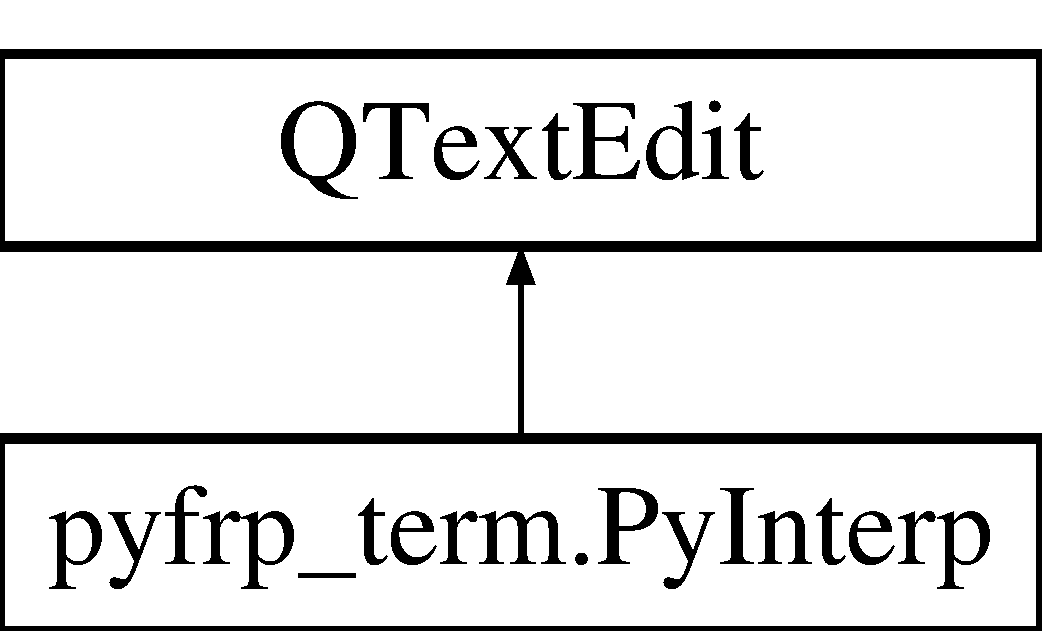
\includegraphics[height=2.000000cm]{classpyfrp__term_1_1PyInterp}
\end{center}
\end{figure}
\subsection*{Classes}
\begin{DoxyCompactItemize}
\item 
class \hyperlink{classpyfrp__term_1_1PyInterp_1_1InteractiveInterpreter}{Interactive\+Interpreter}
\end{DoxyCompactItemize}
\subsection*{Public Member Functions}
\begin{DoxyCompactItemize}
\item 
\hypertarget{classpyfrp__term_1_1PyInterp_ad73f485e863d4b6704bc2b56accafc96}{def {\bfseries \+\_\+\+\_\+init\+\_\+\+\_\+}}\label{classpyfrp__term_1_1PyInterp_ad73f485e863d4b6704bc2b56accafc96}

\item 
\hypertarget{classpyfrp__term_1_1PyInterp_a8e7809ec844863d5b335b795d2ab78c5}{def {\bfseries print\+Banner}}\label{classpyfrp__term_1_1PyInterp_a8e7809ec844863d5b335b795d2ab78c5}

\item 
\hypertarget{classpyfrp__term_1_1PyInterp_a3be4dd9eff91571dbf0c32ac42bc069a}{def {\bfseries marker}}\label{classpyfrp__term_1_1PyInterp_a3be4dd9eff91571dbf0c32ac42bc069a}

\item 
\hypertarget{classpyfrp__term_1_1PyInterp_af3e62bf2e6ca1db533698f3cad5afc95}{def {\bfseries init\+Interpreter}}\label{classpyfrp__term_1_1PyInterp_af3e62bf2e6ca1db533698f3cad5afc95}

\item 
\hypertarget{classpyfrp__term_1_1PyInterp_a03d5c97f73aa2e59ea497cb6cf904650}{def {\bfseries update\+Interpreter\+Locals}}\label{classpyfrp__term_1_1PyInterp_a03d5c97f73aa2e59ea497cb6cf904650}

\item 
\hypertarget{classpyfrp__term_1_1PyInterp_a6c7db193e8b60fdaa066fce652b4516f}{def {\bfseries write}}\label{classpyfrp__term_1_1PyInterp_a6c7db193e8b60fdaa066fce652b4516f}

\item 
\hypertarget{classpyfrp__term_1_1PyInterp_a7bd58066a97069f08e3bab0b04b1d76a}{def {\bfseries clear\+Current\+Block}}\label{classpyfrp__term_1_1PyInterp_a7bd58066a97069f08e3bab0b04b1d76a}

\item 
\hypertarget{classpyfrp__term_1_1PyInterp_a155dcabfbb5fe4726dd042feba91818d}{def {\bfseries recall\+History}}\label{classpyfrp__term_1_1PyInterp_a155dcabfbb5fe4726dd042feba91818d}

\item 
\hypertarget{classpyfrp__term_1_1PyInterp_aa4a790c4a1204dd86ddfb6db4aba3f82}{def {\bfseries custom\+Commands}}\label{classpyfrp__term_1_1PyInterp_aa4a790c4a1204dd86ddfb6db4aba3f82}

\item 
\hypertarget{classpyfrp__term_1_1PyInterp_a4669b4714516bd7453edec674c664252}{def {\bfseries key\+Press\+Event}}\label{classpyfrp__term_1_1PyInterp_a4669b4714516bd7453edec674c664252}

\end{DoxyCompactItemize}
\subsection*{Public Attributes}
\begin{DoxyCompactItemize}
\item 
\hypertarget{classpyfrp__term_1_1PyInterp_a4555438064452a14b36bc5cd542e8e73}{{\bfseries refresh\+Marker}}\label{classpyfrp__term_1_1PyInterp_a4555438064452a14b36bc5cd542e8e73}

\item 
\hypertarget{classpyfrp__term_1_1PyInterp_a18b88274cf6ec0fb9cddc523b6a7fadc}{{\bfseries multi\+Line}}\label{classpyfrp__term_1_1PyInterp_a18b88274cf6ec0fb9cddc523b6a7fadc}

\item 
\hypertarget{classpyfrp__term_1_1PyInterp_a22170ccbb30954cb73199ee147fb2673}{{\bfseries command}}\label{classpyfrp__term_1_1PyInterp_a22170ccbb30954cb73199ee147fb2673}

\item 
\hypertarget{classpyfrp__term_1_1PyInterp_ab3ab46aaa354b0e04c0a396580c72ae4}{{\bfseries history}}\label{classpyfrp__term_1_1PyInterp_ab3ab46aaa354b0e04c0a396580c72ae4}

\item 
\hypertarget{classpyfrp__term_1_1PyInterp_a831e22d99070fbd46e6330e81c7d80c5}{{\bfseries history\+Index}}\label{classpyfrp__term_1_1PyInterp_a831e22d99070fbd46e6330e81c7d80c5}

\item 
\hypertarget{classpyfrp__term_1_1PyInterp_aee07684435a3b88b5fc3ffcd92a3341d}{{\bfseries interpreter\+Locals}}\label{classpyfrp__term_1_1PyInterp_aee07684435a3b88b5fc3ffcd92a3341d}

\item 
\hypertarget{classpyfrp__term_1_1PyInterp_a18bfb5fdefd63b707e18da89b7d64aaa}{{\bfseries interpreter}}\label{classpyfrp__term_1_1PyInterp_a18bfb5fdefd63b707e18da89b7d64aaa}

\item 
\hypertarget{classpyfrp__term_1_1PyInterp_a973aea883afc98f82001af8cfd105804}{{\bfseries have\+Line}}\label{classpyfrp__term_1_1PyInterp_a973aea883afc98f82001af8cfd105804}

\end{DoxyCompactItemize}


The documentation for this class was generated from the following file\+:\begin{DoxyCompactItemize}
\item 
/home/alex\+\_\+loc/\+Documents/\+Research/\+Py\+F\+R\+A\+P/\+Code/pyfrp\+\_\+term.\+py\end{DoxyCompactItemize}

\hypertarget{classpyfrp__subwin_1_1select__fits}{\section{pyfrp\+\_\+subwin.\+select\+\_\+fits Class Reference}
\label{classpyfrp__subwin_1_1select__fits}\index{pyfrp\+\_\+subwin.\+select\+\_\+fits@{pyfrp\+\_\+subwin.\+select\+\_\+fits}}
}
Inheritance diagram for pyfrp\+\_\+subwin.\+select\+\_\+fits\+:\begin{figure}[H]
\begin{center}
\leavevmode
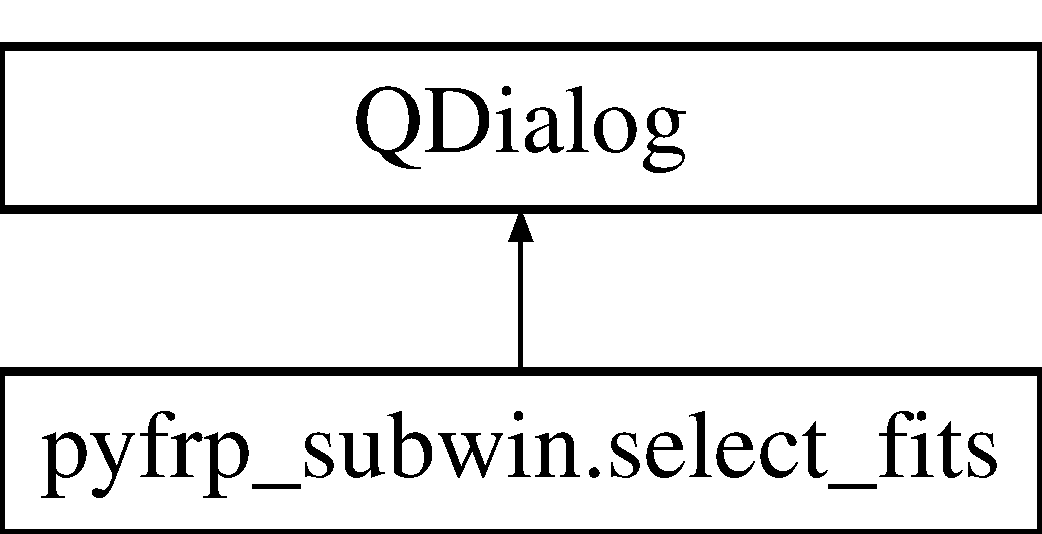
\includegraphics[height=2.000000cm]{classpyfrp__subwin_1_1select__fits}
\end{center}
\end{figure}
\subsection*{Public Member Functions}
\begin{DoxyCompactItemize}
\item 
\hypertarget{classpyfrp__subwin_1_1select__fits_a1fbf0a42586ac5060e7368c6bf387dfc}{def {\bfseries \+\_\+\+\_\+init\+\_\+\+\_\+}}\label{classpyfrp__subwin_1_1select__fits_a1fbf0a42586ac5060e7368c6bf387dfc}

\item 
\hypertarget{classpyfrp__subwin_1_1select__fits_a9a08ea6725b2edeb6456b556e47f90db}{def {\bfseries init\+\_\+left\+\_\+list}}\label{classpyfrp__subwin_1_1select__fits_a9a08ea6725b2edeb6456b556e47f90db}

\item 
\hypertarget{classpyfrp__subwin_1_1select__fits_a17e93205af6f16792eac497f6ed92dd2}{def {\bfseries add\+\_\+fit}}\label{classpyfrp__subwin_1_1select__fits_a17e93205af6f16792eac497f6ed92dd2}

\item 
\hypertarget{classpyfrp__subwin_1_1select__fits_a10c248e3a60ba62f4b52feadbee9d39f}{def {\bfseries remove\+\_\+fit}}\label{classpyfrp__subwin_1_1select__fits_a10c248e3a60ba62f4b52feadbee9d39f}

\item 
\hypertarget{classpyfrp__subwin_1_1select__fits_a68537e6d9f865332a1c39abff56026cc}{def {\bfseries get\+\_\+left\+\_\+selections}}\label{classpyfrp__subwin_1_1select__fits_a68537e6d9f865332a1c39abff56026cc}

\item 
\hypertarget{classpyfrp__subwin_1_1select__fits_a0523bfb927e8b82e02d2f9b7787abf1b}{def {\bfseries get\+\_\+right\+\_\+selections}}\label{classpyfrp__subwin_1_1select__fits_a0523bfb927e8b82e02d2f9b7787abf1b}

\item 
\hypertarget{classpyfrp__subwin_1_1select__fits_aeb9de6990840ef029522b3b45265903c}{def {\bfseries get\+\_\+left\+\_\+ind}}\label{classpyfrp__subwin_1_1select__fits_aeb9de6990840ef029522b3b45265903c}

\item 
\hypertarget{classpyfrp__subwin_1_1select__fits_a94e104ecd93347ed63a67efc37049bcc}{def {\bfseries get\+\_\+right\+\_\+ind}}\label{classpyfrp__subwin_1_1select__fits_a94e104ecd93347ed63a67efc37049bcc}

\item 
\hypertarget{classpyfrp__subwin_1_1select__fits_aa51e38b3ebf4e036050b359d67d44d67}{def {\bfseries done\+\_\+pressed}}\label{classpyfrp__subwin_1_1select__fits_aa51e38b3ebf4e036050b359d67d44d67}

\end{DoxyCompactItemize}
\subsection*{Public Attributes}
\begin{DoxyCompactItemize}
\item 
\hypertarget{classpyfrp__subwin_1_1select__fits_a6e45a53de896ca3fd68b2cc30ce16c8b}{{\bfseries molecule}}\label{classpyfrp__subwin_1_1select__fits_a6e45a53de896ca3fd68b2cc30ce16c8b}

\item 
\hypertarget{classpyfrp__subwin_1_1select__fits_a7d539ad40341adeb07dd85d67c4220f7}{{\bfseries embr\+\_\+in\+\_\+right\+\_\+list}}\label{classpyfrp__subwin_1_1select__fits_a7d539ad40341adeb07dd85d67c4220f7}

\item 
\hypertarget{classpyfrp__subwin_1_1select__fits_a1342b132609defa73e0e4c739f6939d0}{{\bfseries fit\+\_\+in\+\_\+right\+\_\+list}}\label{classpyfrp__subwin_1_1select__fits_a1342b132609defa73e0e4c739f6939d0}

\item 
\hypertarget{classpyfrp__subwin_1_1select__fits_a6e6e8b520a5d63a6a67bcf8de49a2500}{{\bfseries single\+\_\+fit}}\label{classpyfrp__subwin_1_1select__fits_a6e6e8b520a5d63a6a67bcf8de49a2500}

\item 
\hypertarget{classpyfrp__subwin_1_1select__fits_ad41bf3713d84a242df7a16fcaf7f6edb}{{\bfseries btn\+\_\+add}}\label{classpyfrp__subwin_1_1select__fits_ad41bf3713d84a242df7a16fcaf7f6edb}

\item 
\hypertarget{classpyfrp__subwin_1_1select__fits_aa57d2fd6fe4b54427d5b402952591370}{{\bfseries btn\+\_\+remove}}\label{classpyfrp__subwin_1_1select__fits_aa57d2fd6fe4b54427d5b402952591370}

\item 
\hypertarget{classpyfrp__subwin_1_1select__fits_a328ff7c03925a6550f5e817ac721a51a}{{\bfseries btn\+\_\+done}}\label{classpyfrp__subwin_1_1select__fits_a328ff7c03925a6550f5e817ac721a51a}

\item 
\hypertarget{classpyfrp__subwin_1_1select__fits_a5f3cd98d698ed244ada2636f02fea8d8}{{\bfseries left\+\_\+list}}\label{classpyfrp__subwin_1_1select__fits_a5f3cd98d698ed244ada2636f02fea8d8}

\item 
\hypertarget{classpyfrp__subwin_1_1select__fits_adf1c4b2deeaf9ae6beac4f7f8d4aed31}{{\bfseries right\+\_\+list}}\label{classpyfrp__subwin_1_1select__fits_adf1c4b2deeaf9ae6beac4f7f8d4aed31}

\item 
\hypertarget{classpyfrp__subwin_1_1select__fits_a90d470b7ab5e1c22e751fc28aeb742b5}{{\bfseries vbox}}\label{classpyfrp__subwin_1_1select__fits_a90d470b7ab5e1c22e751fc28aeb742b5}

\item 
\hypertarget{classpyfrp__subwin_1_1select__fits_ae5b590957cf50f1b05ed87ff349f4db2}{{\bfseries hbox}}\label{classpyfrp__subwin_1_1select__fits_ae5b590957cf50f1b05ed87ff349f4db2}

\item 
\hypertarget{classpyfrp__subwin_1_1select__fits_a907fa7dc424414159af42a723a61e8ab}{{\bfseries vbox2}}\label{classpyfrp__subwin_1_1select__fits_a907fa7dc424414159af42a723a61e8ab}

\item 
\hypertarget{classpyfrp__subwin_1_1select__fits_ac5a4780e0c6122960ce17ea6088b2322}{{\bfseries curr\+\_\+embr\+\_\+node}}\label{classpyfrp__subwin_1_1select__fits_ac5a4780e0c6122960ce17ea6088b2322}

\item 
\hypertarget{classpyfrp__subwin_1_1select__fits_a891057c28371ff1daa0f206eee20d4f2}{{\bfseries curr\+\_\+embr}}\label{classpyfrp__subwin_1_1select__fits_a891057c28371ff1daa0f206eee20d4f2}

\item 
\hypertarget{classpyfrp__subwin_1_1select__fits_a4262a7c8e85d6b363aaec9f15fe2d750}{{\bfseries curr\+\_\+fit}}\label{classpyfrp__subwin_1_1select__fits_a4262a7c8e85d6b363aaec9f15fe2d750}

\item 
\hypertarget{classpyfrp__subwin_1_1select__fits_a958b2fdb6cd4d2e647da53a44d57a9f2}{{\bfseries curr\+\_\+fit\+\_\+node}}\label{classpyfrp__subwin_1_1select__fits_a958b2fdb6cd4d2e647da53a44d57a9f2}

\item 
\hypertarget{classpyfrp__subwin_1_1select__fits_a8fa3670eb0c305db232620fb4a452f7b}{{\bfseries curr\+\_\+target\+\_\+embr\+\_\+node}}\label{classpyfrp__subwin_1_1select__fits_a8fa3670eb0c305db232620fb4a452f7b}

\item 
\hypertarget{classpyfrp__subwin_1_1select__fits_a2f5e8f4ef911dfefd79881d4e7bd0078}{{\bfseries curr\+\_\+target\+\_\+fit\+\_\+node}}\label{classpyfrp__subwin_1_1select__fits_a2f5e8f4ef911dfefd79881d4e7bd0078}

\item 
\hypertarget{classpyfrp__subwin_1_1select__fits_a68734016f3ca399ba96727341c28d4fe}{{\bfseries curr\+\_\+target\+\_\+fit}}\label{classpyfrp__subwin_1_1select__fits_a68734016f3ca399ba96727341c28d4fe}

\end{DoxyCompactItemize}


The documentation for this class was generated from the following file\+:\begin{DoxyCompactItemize}
\item 
/home/alex\+\_\+loc/\+Documents/\+Research/\+Py\+F\+R\+A\+P/\+Code/pyfrp\+\_\+subwin.\+py\end{DoxyCompactItemize}

\hypertarget{classpyfrp__subwin_1_1sim__dialog}{\section{pyfrp\+\_\+subwin.\+sim\+\_\+dialog Class Reference}
\label{classpyfrp__subwin_1_1sim__dialog}\index{pyfrp\+\_\+subwin.\+sim\+\_\+dialog@{pyfrp\+\_\+subwin.\+sim\+\_\+dialog}}
}
Inheritance diagram for pyfrp\+\_\+subwin.\+sim\+\_\+dialog\+:\begin{figure}[H]
\begin{center}
\leavevmode
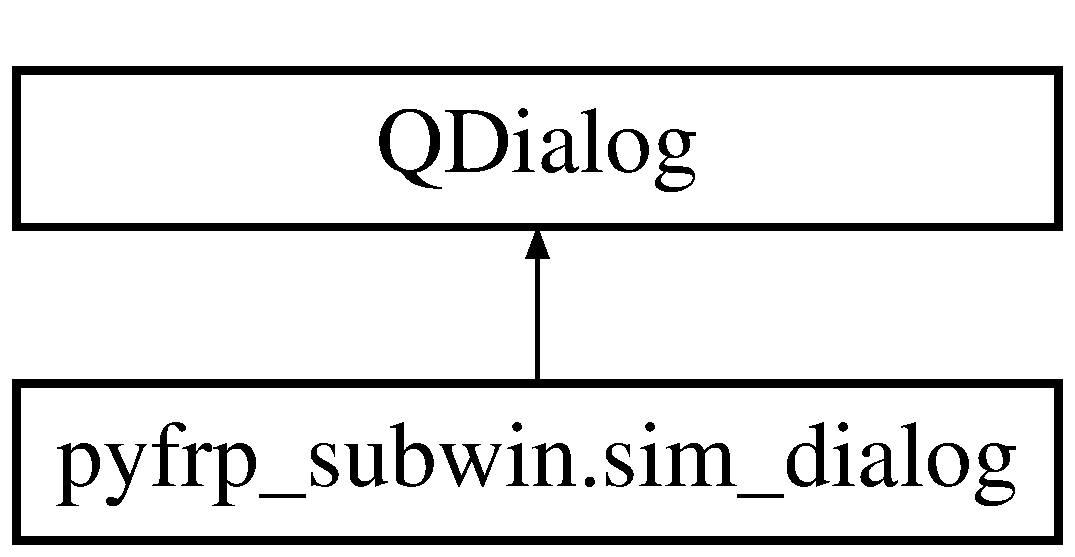
\includegraphics[height=2.000000cm]{classpyfrp__subwin_1_1sim__dialog}
\end{center}
\end{figure}
\subsection*{Public Member Functions}
\begin{DoxyCompactItemize}
\item 
\hypertarget{classpyfrp__subwin_1_1sim__dialog_a144b65d6ee5f8ad7323ec28b9962ff07}{def {\bfseries \+\_\+\+\_\+init\+\_\+\+\_\+}}\label{classpyfrp__subwin_1_1sim__dialog_a144b65d6ee5f8ad7323ec28b9962ff07}

\item 
\hypertarget{classpyfrp__subwin_1_1sim__dialog_ad3403e20aa87699cb2f349b34a133c67}{def {\bfseries sel\+\_\+avg}}\label{classpyfrp__subwin_1_1sim__dialog_ad3403e20aa87699cb2f349b34a133c67}

\item 
\hypertarget{classpyfrp__subwin_1_1sim__dialog_a1edbd9375f9bfa25d6c22dad0f9056ce}{def {\bfseries sel\+\_\+int}}\label{classpyfrp__subwin_1_1sim__dialog_a1edbd9375f9bfa25d6c22dad0f9056ce}

\item 
\hypertarget{classpyfrp__subwin_1_1sim__dialog_a606c4e5212dc5404248a003e4a83c195}{def {\bfseries sel\+\_\+ic}}\label{classpyfrp__subwin_1_1sim__dialog_a606c4e5212dc5404248a003e4a83c195}

\item 
\hypertarget{classpyfrp__subwin_1_1sim__dialog_a797fd3deda531725f889730e06a5674a}{def {\bfseries set\+\_\+rad\+\_\+steps}}\label{classpyfrp__subwin_1_1sim__dialog_a797fd3deda531725f889730e06a5674a}

\item 
\hypertarget{classpyfrp__subwin_1_1sim__dialog_a56f42ea948e89f3423a383ffdc07cb12}{def {\bfseries set\+\_\+int\+\_\+steps}}\label{classpyfrp__subwin_1_1sim__dialog_a56f42ea948e89f3423a383ffdc07cb12}

\item 
\hypertarget{classpyfrp__subwin_1_1sim__dialog_a99ee039cbf83679162d49ba1d588f5de}{def {\bfseries set\+\_\+volsize}}\label{classpyfrp__subwin_1_1sim__dialog_a99ee039cbf83679162d49ba1d588f5de}

\item 
\hypertarget{classpyfrp__subwin_1_1sim__dialog_a7a15b8e5ff178b3de8c1864371e562e4}{def {\bfseries set\+\_\+diff}}\label{classpyfrp__subwin_1_1sim__dialog_a7a15b8e5ff178b3de8c1864371e562e4}

\item 
\hypertarget{classpyfrp__subwin_1_1sim__dialog_aa714bae65fc3f6060491d79f9f1d5aa7}{def {\bfseries set\+\_\+prod}}\label{classpyfrp__subwin_1_1sim__dialog_aa714bae65fc3f6060491d79f9f1d5aa7}

\item 
\hypertarget{classpyfrp__subwin_1_1sim__dialog_a0a1bda0c55f7d1f647d78585803dcfbf}{def {\bfseries set\+\_\+degr}}\label{classpyfrp__subwin_1_1sim__dialog_a0a1bda0c55f7d1f647d78585803dcfbf}

\item 
\hypertarget{classpyfrp__subwin_1_1sim__dialog_ab5163e1295f81bacb96b7766c2e66ddc}{def {\bfseries set\+\_\+steps}}\label{classpyfrp__subwin_1_1sim__dialog_ab5163e1295f81bacb96b7766c2e66ddc}

\item 
\hypertarget{classpyfrp__subwin_1_1sim__dialog_ad1636436fc73f8ced4ba45a8ea98f14e}{def {\bfseries check\+\_\+usemesh}}\label{classpyfrp__subwin_1_1sim__dialog_ad1636436fc73f8ced4ba45a8ea98f14e}

\item 
\hypertarget{classpyfrp__subwin_1_1sim__dialog_ae9944fd15a2ef67455244186313564b3}{def {\bfseries check\+\_\+add\+\_\+rim\+\_\+sim}}\label{classpyfrp__subwin_1_1sim__dialog_ae9944fd15a2ef67455244186313564b3}

\item 
\hypertarget{classpyfrp__subwin_1_1sim__dialog_aa02860148b8477095abe3da7ebdd67f1}{def {\bfseries check\+\_\+small}}\label{classpyfrp__subwin_1_1sim__dialog_aa02860148b8477095abe3da7ebdd67f1}

\item 
\hypertarget{classpyfrp__subwin_1_1sim__dialog_abf905a3941d043571d868eede7a8f3f0}{def {\bfseries check\+\_\+debug\+\_\+all}}\label{classpyfrp__subwin_1_1sim__dialog_abf905a3941d043571d868eede7a8f3f0}

\item 
\hypertarget{classpyfrp__subwin_1_1sim__dialog_a5d9ffe132c94941b79a436dc9e1498ca}{def {\bfseries sel\+\_\+fn\+\_\+mesh}}\label{classpyfrp__subwin_1_1sim__dialog_a5d9ffe132c94941b79a436dc9e1498ca}

\item 
\hypertarget{classpyfrp__subwin_1_1sim__dialog_a868836cfbf31bdd918d5787760956999}{def {\bfseries done\+\_\+pressed}}\label{classpyfrp__subwin_1_1sim__dialog_a868836cfbf31bdd918d5787760956999}

\end{DoxyCompactItemize}
\subsection*{Public Attributes}
\begin{DoxyCompactItemize}
\item 
\hypertarget{classpyfrp__subwin_1_1sim__dialog_ab2ae5a5a5e9ab8e54fdc0025ed42e58d}{{\bfseries embryo}}\label{classpyfrp__subwin_1_1sim__dialog_ab2ae5a5a5e9ab8e54fdc0025ed42e58d}

\item 
\hypertarget{classpyfrp__subwin_1_1sim__dialog_ab371994261d4efe615ade74f7fe81cd5}{{\bfseries btn\+\_\+done}}\label{classpyfrp__subwin_1_1sim__dialog_ab371994261d4efe615ade74f7fe81cd5}

\item 
\hypertarget{classpyfrp__subwin_1_1sim__dialog_a218e2bff28896ec825df0990c7ad5d01}{{\bfseries btn\+\_\+fn\+\_\+mesh}}\label{classpyfrp__subwin_1_1sim__dialog_a218e2bff28896ec825df0990c7ad5d01}

\item 
\hypertarget{classpyfrp__subwin_1_1sim__dialog_a26908430afbe3dc1aefe63c91060470a}{{\bfseries lbl\+\_\+parms}}\label{classpyfrp__subwin_1_1sim__dialog_a26908430afbe3dc1aefe63c91060470a}

\item 
\hypertarget{classpyfrp__subwin_1_1sim__dialog_ace0217add0cc26ee2b4cb26b365a6cf0}{{\bfseries lbl\+\_\+ics}}\label{classpyfrp__subwin_1_1sim__dialog_ace0217add0cc26ee2b4cb26b365a6cf0}

\item 
\hypertarget{classpyfrp__subwin_1_1sim__dialog_a2e4f0752b804a3ec328fb5b142074e2e}{{\bfseries lbl\+\_\+avging}}\label{classpyfrp__subwin_1_1sim__dialog_a2e4f0752b804a3ec328fb5b142074e2e}

\item 
\hypertarget{classpyfrp__subwin_1_1sim__dialog_abb0892853915077f88e9eecc1e688100}{{\bfseries lbl\+\_\+mesh}}\label{classpyfrp__subwin_1_1sim__dialog_abb0892853915077f88e9eecc1e688100}

\item 
\hypertarget{classpyfrp__subwin_1_1sim__dialog_a29c67b0916bd678289e60e96b8c2d9cc}{{\bfseries lbl\+\_\+debugging}}\label{classpyfrp__subwin_1_1sim__dialog_a29c67b0916bd678289e60e96b8c2d9cc}

\item 
\hypertarget{classpyfrp__subwin_1_1sim__dialog_aeee65d9ec6a0a55422721bf85590a645}{{\bfseries lbl\+\_\+diff}}\label{classpyfrp__subwin_1_1sim__dialog_aeee65d9ec6a0a55422721bf85590a645}

\item 
\hypertarget{classpyfrp__subwin_1_1sim__dialog_a4c5d81f695ec492e203c03c7248a682b}{{\bfseries lbl\+\_\+prod}}\label{classpyfrp__subwin_1_1sim__dialog_a4c5d81f695ec492e203c03c7248a682b}

\item 
\hypertarget{classpyfrp__subwin_1_1sim__dialog_a92ff115cdf7687e097c02c6dda1b2b22}{{\bfseries lbl\+\_\+degr}}\label{classpyfrp__subwin_1_1sim__dialog_a92ff115cdf7687e097c02c6dda1b2b22}

\item 
\hypertarget{classpyfrp__subwin_1_1sim__dialog_ae5d741d2bd94568d102f889f60051774}{{\bfseries lbl\+\_\+steps}}\label{classpyfrp__subwin_1_1sim__dialog_ae5d741d2bd94568d102f889f60051774}

\item 
\hypertarget{classpyfrp__subwin_1_1sim__dialog_a72a081e5ddc54b190c82fd8df9cb364b}{{\bfseries lbl\+\_\+tstart}}\label{classpyfrp__subwin_1_1sim__dialog_a72a081e5ddc54b190c82fd8df9cb364b}

\item 
\hypertarget{classpyfrp__subwin_1_1sim__dialog_a94cf660e22f23262a9b9145d741b286e}{{\bfseries lbl\+\_\+tend}}\label{classpyfrp__subwin_1_1sim__dialog_a94cf660e22f23262a9b9145d741b286e}

\item 
\hypertarget{classpyfrp__subwin_1_1sim__dialog_af0e92b44d205bdd4338e62bc231cffec}{{\bfseries lbl\+\_\+\+I\+C\+\_\+mode}}\label{classpyfrp__subwin_1_1sim__dialog_af0e92b44d205bdd4338e62bc231cffec}

\item 
\hypertarget{classpyfrp__subwin_1_1sim__dialog_ab9392923b6be3765ed78a6c96581d42f}{{\bfseries lbl\+\_\+rad\+\_\+steps}}\label{classpyfrp__subwin_1_1sim__dialog_ab9392923b6be3765ed78a6c96581d42f}

\item 
\hypertarget{classpyfrp__subwin_1_1sim__dialog_ab2deb2b33e03cd24991e5e884a9bf269}{{\bfseries lbl\+\_\+avg\+\_\+meth}}\label{classpyfrp__subwin_1_1sim__dialog_ab2deb2b33e03cd24991e5e884a9bf269}

\item 
\hypertarget{classpyfrp__subwin_1_1sim__dialog_a4c4924f99e7d2c1ccfeb6dd949a9ba44}{{\bfseries lbl\+\_\+small}}\label{classpyfrp__subwin_1_1sim__dialog_a4c4924f99e7d2c1ccfeb6dd949a9ba44}

\item 
\hypertarget{classpyfrp__subwin_1_1sim__dialog_a35141d812e9590063b16e365816862bb}{{\bfseries lbl\+\_\+int\+\_\+meth}}\label{classpyfrp__subwin_1_1sim__dialog_a35141d812e9590063b16e365816862bb}

\item 
\hypertarget{classpyfrp__subwin_1_1sim__dialog_afc4b13bf52e6bc3c9d7c072e72bfcb66}{{\bfseries lbl\+\_\+add\+\_\+rim\+\_\+sim}}\label{classpyfrp__subwin_1_1sim__dialog_afc4b13bf52e6bc3c9d7c072e72bfcb66}

\item 
\hypertarget{classpyfrp__subwin_1_1sim__dialog_af1cd908ff99457205567c4634c8e002b}{{\bfseries lbl\+\_\+int\+\_\+steps}}\label{classpyfrp__subwin_1_1sim__dialog_af1cd908ff99457205567c4634c8e002b}

\item 
\hypertarget{classpyfrp__subwin_1_1sim__dialog_aed9cbd23b4c9ccceebe9fe0670a382ed}{{\bfseries lbl\+\_\+volsize}}\label{classpyfrp__subwin_1_1sim__dialog_aed9cbd23b4c9ccceebe9fe0670a382ed}

\item 
\hypertarget{classpyfrp__subwin_1_1sim__dialog_a980d1cdecd547baef6164c6d2afcc17b}{{\bfseries lbl\+\_\+usemesh}}\label{classpyfrp__subwin_1_1sim__dialog_a980d1cdecd547baef6164c6d2afcc17b}

\item 
\hypertarget{classpyfrp__subwin_1_1sim__dialog_afe25e84fe33213c26046175446fec389}{{\bfseries lbl\+\_\+name\+\_\+fn\+\_\+mesh}}\label{classpyfrp__subwin_1_1sim__dialog_afe25e84fe33213c26046175446fec389}

\item 
\hypertarget{classpyfrp__subwin_1_1sim__dialog_a168edbda768c83ea46e63b9bf99c323a}{{\bfseries lbl\+\_\+fn\+\_\+mesh}}\label{classpyfrp__subwin_1_1sim__dialog_a168edbda768c83ea46e63b9bf99c323a}

\item 
\hypertarget{classpyfrp__subwin_1_1sim__dialog_a74f05f44281e6273c8a08ea4bde9319c}{{\bfseries lbl\+\_\+debug\+\_\+all}}\label{classpyfrp__subwin_1_1sim__dialog_a74f05f44281e6273c8a08ea4bde9319c}

\item 
\hypertarget{classpyfrp__subwin_1_1sim__dialog_a617992ce1446466cb89bfbc8d4b519a8}{{\bfseries lbl\+\_\+debug\+\_\+interp}}\label{classpyfrp__subwin_1_1sim__dialog_a617992ce1446466cb89bfbc8d4b519a8}

\item 
\hypertarget{classpyfrp__subwin_1_1sim__dialog_ac169f7b7f84da81da069a14178d7e85d}{{\bfseries lbl\+\_\+debug\+\_\+integr}}\label{classpyfrp__subwin_1_1sim__dialog_ac169f7b7f84da81da069a14178d7e85d}

\item 
\hypertarget{classpyfrp__subwin_1_1sim__dialog_abfbe8fe3ab3ae7e1e73af153f36d4cb7}{{\bfseries lbl\+\_\+debug\+\_\+out}}\label{classpyfrp__subwin_1_1sim__dialog_abfbe8fe3ab3ae7e1e73af153f36d4cb7}

\item 
\hypertarget{classpyfrp__subwin_1_1sim__dialog_ae0954e4c4129f409e80cc6ed6c0a66d2}{{\bfseries cb\+\_\+small}}\label{classpyfrp__subwin_1_1sim__dialog_ae0954e4c4129f409e80cc6ed6c0a66d2}

\item 
\hypertarget{classpyfrp__subwin_1_1sim__dialog_abd09b3b974da51d9b9a74144d841967a}{{\bfseries cb\+\_\+add\+\_\+rim\+\_\+sim}}\label{classpyfrp__subwin_1_1sim__dialog_abd09b3b974da51d9b9a74144d841967a}

\item 
\hypertarget{classpyfrp__subwin_1_1sim__dialog_ad4607b60a63be6e0e3bbd000081091fa}{{\bfseries cb\+\_\+usemesh}}\label{classpyfrp__subwin_1_1sim__dialog_ad4607b60a63be6e0e3bbd000081091fa}

\item 
\hypertarget{classpyfrp__subwin_1_1sim__dialog_a9aa8a805842c1dc363133d3212ad668d}{{\bfseries cb\+\_\+debug\+\_\+all}}\label{classpyfrp__subwin_1_1sim__dialog_a9aa8a805842c1dc363133d3212ad668d}

\item 
\hypertarget{classpyfrp__subwin_1_1sim__dialog_a08e14e0f275d5a3aa76b22c89718159d}{{\bfseries cb\+\_\+debug\+\_\+interp}}\label{classpyfrp__subwin_1_1sim__dialog_a08e14e0f275d5a3aa76b22c89718159d}

\item 
\hypertarget{classpyfrp__subwin_1_1sim__dialog_a8dfddce109c1a164f98bde72f58efdc9}{{\bfseries cb\+\_\+debug\+\_\+integr}}\label{classpyfrp__subwin_1_1sim__dialog_a8dfddce109c1a164f98bde72f58efdc9}

\item 
\hypertarget{classpyfrp__subwin_1_1sim__dialog_ae596a45f9910bba34403bb0f6d3acb82}{{\bfseries cb\+\_\+debug\+\_\+out}}\label{classpyfrp__subwin_1_1sim__dialog_ae596a45f9910bba34403bb0f6d3acb82}

\item 
\hypertarget{classpyfrp__subwin_1_1sim__dialog_a679d6327a23710c5188de6e68f6650cb}{{\bfseries qle\+\_\+diff}}\label{classpyfrp__subwin_1_1sim__dialog_a679d6327a23710c5188de6e68f6650cb}

\item 
\hypertarget{classpyfrp__subwin_1_1sim__dialog_a726d7192d79b02a8de2240b1f43a72f2}{{\bfseries qle\+\_\+prod}}\label{classpyfrp__subwin_1_1sim__dialog_a726d7192d79b02a8de2240b1f43a72f2}

\item 
\hypertarget{classpyfrp__subwin_1_1sim__dialog_a9dfdfc2109b3974cbe8afa50bedc502a}{{\bfseries qle\+\_\+degr}}\label{classpyfrp__subwin_1_1sim__dialog_a9dfdfc2109b3974cbe8afa50bedc502a}

\item 
\hypertarget{classpyfrp__subwin_1_1sim__dialog_acf084f7855274495590155d22078dfe7}{{\bfseries qle\+\_\+steps}}\label{classpyfrp__subwin_1_1sim__dialog_acf084f7855274495590155d22078dfe7}

\item 
\hypertarget{classpyfrp__subwin_1_1sim__dialog_aa87a6431e4bb92cdf6bf046ebfc91061}{{\bfseries qle\+\_\+tstart}}\label{classpyfrp__subwin_1_1sim__dialog_aa87a6431e4bb92cdf6bf046ebfc91061}

\item 
\hypertarget{classpyfrp__subwin_1_1sim__dialog_a6fe10da8e4ee56720fb0fca035faa00b}{{\bfseries qle\+\_\+tend}}\label{classpyfrp__subwin_1_1sim__dialog_a6fe10da8e4ee56720fb0fca035faa00b}

\item 
\hypertarget{classpyfrp__subwin_1_1sim__dialog_a778b8c42d8ca2100c335838339b59064}{{\bfseries qle\+\_\+int\+\_\+steps}}\label{classpyfrp__subwin_1_1sim__dialog_a778b8c42d8ca2100c335838339b59064}

\item 
\hypertarget{classpyfrp__subwin_1_1sim__dialog_ab1002e704857e22921d5f70aedd489b0}{{\bfseries qle\+\_\+rad\+\_\+steps}}\label{classpyfrp__subwin_1_1sim__dialog_ab1002e704857e22921d5f70aedd489b0}

\item 
\hypertarget{classpyfrp__subwin_1_1sim__dialog_aff65ccaa602d813b11c19c326662e5bc}{{\bfseries qle\+\_\+volsize}}\label{classpyfrp__subwin_1_1sim__dialog_aff65ccaa602d813b11c19c326662e5bc}

\item 
\hypertarget{classpyfrp__subwin_1_1sim__dialog_a649bfe826ba8a8fda249778044c20d69}{{\bfseries double\+\_\+valid}}\label{classpyfrp__subwin_1_1sim__dialog_a649bfe826ba8a8fda249778044c20d69}

\item 
\hypertarget{classpyfrp__subwin_1_1sim__dialog_ab32bb50bc61b885e0501d85e637c366e}{{\bfseries combo\+\_\+ic}}\label{classpyfrp__subwin_1_1sim__dialog_ab32bb50bc61b885e0501d85e637c366e}

\item 
\hypertarget{classpyfrp__subwin_1_1sim__dialog_aad9df19eb21297a170f854df2a267bab}{{\bfseries combo\+\_\+avg}}\label{classpyfrp__subwin_1_1sim__dialog_aad9df19eb21297a170f854df2a267bab}

\item 
\hypertarget{classpyfrp__subwin_1_1sim__dialog_af1ead9298e7c195842039082a96d69fa}{{\bfseries combo\+\_\+int}}\label{classpyfrp__subwin_1_1sim__dialog_af1ead9298e7c195842039082a96d69fa}

\end{DoxyCompactItemize}


The documentation for this class was generated from the following file\+:\begin{DoxyCompactItemize}
\item 
/home/alex\+\_\+loc/\+Documents/\+Research/\+Py\+F\+R\+A\+P/\+Code/pyfrp\+\_\+subwin.\+py\end{DoxyCompactItemize}

\hypertarget{classpyfrp__subwin_1_1simulation__prog}{\section{pyfrp\+\_\+subwin.\+simulation\+\_\+prog Class Reference}
\label{classpyfrp__subwin_1_1simulation__prog}\index{pyfrp\+\_\+subwin.\+simulation\+\_\+prog@{pyfrp\+\_\+subwin.\+simulation\+\_\+prog}}
}
Inheritance diagram for pyfrp\+\_\+subwin.\+simulation\+\_\+prog\+:\begin{figure}[H]
\begin{center}
\leavevmode
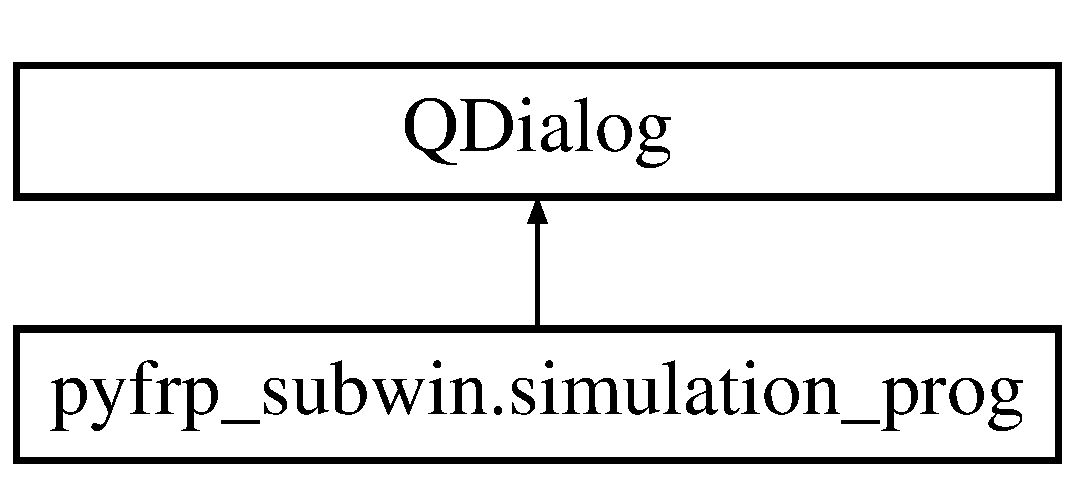
\includegraphics[height=2.000000cm]{classpyfrp__subwin_1_1simulation__prog}
\end{center}
\end{figure}
\subsection*{Public Member Functions}
\begin{DoxyCompactItemize}
\item 
\hypertarget{classpyfrp__subwin_1_1simulation__prog_a5288d7ba12248a15dfe0e8f045676b77}{def {\bfseries \+\_\+\+\_\+init\+\_\+\+\_\+}}\label{classpyfrp__subwin_1_1simulation__prog_a5288d7ba12248a15dfe0e8f045676b77}

\item 
\hypertarget{classpyfrp__subwin_1_1simulation__prog_a851e30de5c542d5d3e36101f0e4b6e6b}{def {\bfseries cancel\+\_\+simulation}}\label{classpyfrp__subwin_1_1simulation__prog_a851e30de5c542d5d3e36101f0e4b6e6b}

\end{DoxyCompactItemize}
\subsection*{Public Attributes}
\begin{DoxyCompactItemize}
\item 
\hypertarget{classpyfrp__subwin_1_1simulation__prog_a48efd7edeedbb14a5d428429af1c718f}{{\bfseries lbl\+\_\+name}}\label{classpyfrp__subwin_1_1simulation__prog_a48efd7edeedbb14a5d428429af1c718f}

\item 
\hypertarget{classpyfrp__subwin_1_1simulation__prog_a8dbd40225b6f21db3ce5335cf43113b3}{{\bfseries btn\+\_\+cancel}}\label{classpyfrp__subwin_1_1simulation__prog_a8dbd40225b6f21db3ce5335cf43113b3}

\item 
\hypertarget{classpyfrp__subwin_1_1simulation__prog_ad949a9cfe62bd24a7a1122df312aa8a1}{{\bfseries progressbar}}\label{classpyfrp__subwin_1_1simulation__prog_ad949a9cfe62bd24a7a1122df312aa8a1}

\item 
\hypertarget{classpyfrp__subwin_1_1simulation__prog_a6261d29ef6bd6511c9c7da0d8c3de6a7}{{\bfseries vbox}}\label{classpyfrp__subwin_1_1simulation__prog_a6261d29ef6bd6511c9c7da0d8c3de6a7}

\end{DoxyCompactItemize}


The documentation for this class was generated from the following file\+:\begin{DoxyCompactItemize}
\item 
/home/alex\+\_\+loc/\+Documents/\+Research/\+Py\+F\+R\+A\+P/\+Code/pyfrp\+\_\+subwin.\+py\end{DoxyCompactItemize}

\hypertarget{classpyfrp__subwin_1_1simulation__thread}{\section{pyfrp\+\_\+subwin.\+simulation\+\_\+thread Class Reference}
\label{classpyfrp__subwin_1_1simulation__thread}\index{pyfrp\+\_\+subwin.\+simulation\+\_\+thread@{pyfrp\+\_\+subwin.\+simulation\+\_\+thread}}
}
Inheritance diagram for pyfrp\+\_\+subwin.\+simulation\+\_\+thread\+:\begin{figure}[H]
\begin{center}
\leavevmode
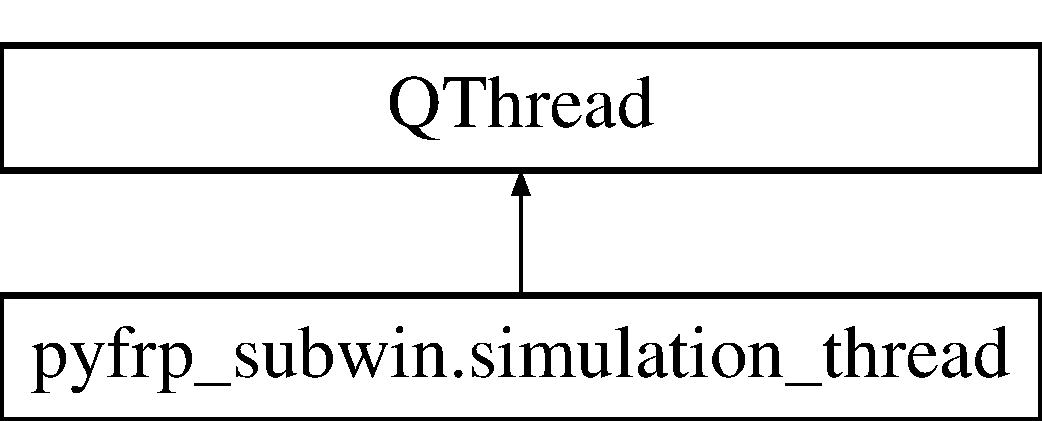
\includegraphics[height=2.000000cm]{classpyfrp__subwin_1_1simulation__thread}
\end{center}
\end{figure}
\subsection*{Public Member Functions}
\begin{DoxyCompactItemize}
\item 
\hypertarget{classpyfrp__subwin_1_1simulation__thread_a35791374002f347d264c403f58438a48}{def {\bfseries \+\_\+\+\_\+init\+\_\+\+\_\+}}\label{classpyfrp__subwin_1_1simulation__thread_a35791374002f347d264c403f58438a48}

\item 
\hypertarget{classpyfrp__subwin_1_1simulation__thread_a5efcac439e906c4e25a906e55978fcd3}{def {\bfseries \+\_\+\+\_\+del\+\_\+\+\_\+}}\label{classpyfrp__subwin_1_1simulation__thread_a5efcac439e906c4e25a906e55978fcd3}

\item 
\hypertarget{classpyfrp__subwin_1_1simulation__thread_a99ae824712e6805340e07f07b9594ec3}{def {\bfseries run}}\label{classpyfrp__subwin_1_1simulation__thread_a99ae824712e6805340e07f07b9594ec3}

\end{DoxyCompactItemize}
\subsection*{Public Attributes}
\begin{DoxyCompactItemize}
\item 
\hypertarget{classpyfrp__subwin_1_1simulation__thread_a44926d141eb3e5b215cd80130b97401e}{{\bfseries embryo}}\label{classpyfrp__subwin_1_1simulation__thread_a44926d141eb3e5b215cd80130b97401e}

\end{DoxyCompactItemize}
\subsection*{Static Public Attributes}
\begin{DoxyCompactItemize}
\item 
\hypertarget{classpyfrp__subwin_1_1simulation__thread_acaefa646cabdcd360614eacb624c74ec}{tuple {\bfseries task\+Finished} = Qt\+Core.\+pyqt\+Signal()}\label{classpyfrp__subwin_1_1simulation__thread_acaefa646cabdcd360614eacb624c74ec}

\item 
\hypertarget{classpyfrp__subwin_1_1simulation__thread_a8fcdacdbced51ca71d10117d393179f0}{tuple {\bfseries prog\+\_\+signal} = Qt\+Core.\+pyqt\+Signal(int)}\label{classpyfrp__subwin_1_1simulation__thread_a8fcdacdbced51ca71d10117d393179f0}

\end{DoxyCompactItemize}


The documentation for this class was generated from the following file\+:\begin{DoxyCompactItemize}
\item 
/home/alex\+\_\+loc/\+Documents/\+Research/\+Py\+F\+R\+A\+P/\+Code/pyfrp\+\_\+subwin.\+py\end{DoxyCompactItemize}

%--- End generated contents ---

% Index
\newpage
\phantomsection
\addcontentsline{toc}{chapter}{Index}
\printindex

\end{document}
